 
% ------------------------------------------------- -----
% ------------------------------------------------- -----
% Correction of exo                           
% ------------------------------------------------- -----
% ------------------------------------------------- -----
 
\chapter{Correction of exercises}
 
% \addcontentsline{toc}{chapter}{Correction of exercises}
\section{Correction of the exercises of chapter 1}
 
 
\begin{correction}{exo-determinant-circulating}
\index{Determinant!circulating} \begin{enumerate}
\item Let $ \chi \in \wh{G} $. The convolution theorem \ref{thm-convolution-trans-fourier-grpe-abelien}, tells us that $ \Ff(f * \chi) = \wh{f} \cdot \wh{\chi} $. We easily verify that $ \wh{\chi} = |G| \delta_{\chi^{-1}} $, where $ \delta_{\chi^{-1}} \in \CC [\wh{G}] $ is the function that equals $ 1 $ in $ \chi^{-1} $ and $ 0 $ otherwise. This allows us to write that $ \Ff(f * \chi) = |G| \wh{f} (\chi^{-1}) \delta_{\chi^{-1}} $. It only remains to apply the inverse Fourier transform using the fact that $ \Ff^{-1} (\delta_{\chi^{-1}}) = \tfrac{1}{G} \chi $. We thus obtain that $ \Phi^f(\chi) = f * \chi = \wh{f} (\chi^{-1}) \chi $. So $ \chi $ is an eigenvector for $ \Phi^f $, with associated eigenvalue $ \wh{f} (\chi^{-1}) $.
\item We have $ \Phi^f(\delta_g) = f * \delta_g = \sum_{h \in G}{f(g^{-1} h) \delta_{h}} $. If we write $ \{0, \ldots, \, n-1\} $ the elements of $ G \simeq \ZZ/n \ZZ $, we write the matrix $ A = \{a_{ij}\} $ in the form $ a_{ij} = f(ij) $. \\Moreover, with the previous question, we have the expression of the determinant
\begin{equation*}
\det (A) = \prod_{\chi \in \wh{G}}{\wh{f} (\chi^{-1})} = \prod_{\chi \in \wh{G}}{\wh{f} (\chi)}.
\end{equation*}
 
\item Just choose $ G = \ZZ/n \ZZ $, as well as $ \forall i \in \ZZ/n \ZZ $, $ f(i) = a_i $.
\item We can compute $ \wh{f} $ in $ O(n \log (n)) $ operations with the FFT algorithm, and we obtain the determinant by multiplying the inputs of $ \wh{f} between them $. The \Matlab{} \ref{listing-calcul-det-circ} program does this, on a vector $ f $ of size 10 drawn at random.
 
\begin{listing} \begin{footnotesize}
{\upshape
\begin{tabular}{l} \texttt{n = 10; f = rand (n, 1);} \\
\texttt{prod(fft(f))} \\
\end{tabular}
}
\end{footnotesize}
\caption{Calculation of circulating determinant}
\label{listing-calcul-det-circ}
\end{listing}
 
\end{enumerate}
\end{correction}
 
 
\begin{correction}{exo-dual-so3}
\begin{enumerate}
\item We consider $ R_1 $ (resp. $ R_2 $) a rotation of unit axis $ u_1 $ (resp. $ u_2 $), as well as $ v_1, \, w_1 $ (resp. $ v_2, \, w_2 $ ) an orthonormal basis of the plane $ (u_1)^\bot $ (resp. $ (u_2)^\bot $). We take $ \Omega $ the isometry which sends $ (u_1, \, v_1, \, w_1) $ on $ (u_2, \, v_2, \, w_2) $. If the two rotations have the same angle, we have $ R_1 = \Omega^* R_2 \Omega $.
\item Like $ \chi (a^{-1} ba) = \chi (a)^{-1} \chi (b) \chi (a) = \chi (b) $, $ \chi $ is constant on conjugation classes. With the previous question, $ \chi (R) $ depends only on the angle of the rotation $ R $.
\item \index{Trace} We use the fact that $ \tr (t_\beta) = 1 + 2 \cos (\beta) $. By doing the calculation (with \textsc{Maple}, as shown in \listingterme{} \ref{listing-calcul-trace-beta}), we find that $ \tr (r_{\alpha} s_{\alpha}^{-1}) = 2 \cos (\alpha) + \cos (\alpha)^2 $.
 
\begin{listing} \begin{footnotesize}
{\upshape
\begin{tabular}{l} \texttt{\pwith{} (linalg):} \\
\texttt{r1:= matrix(3,3, [1,0,0,0, cos (t), sin(t), 0, -sin(t), cos (t)]);} \\
\texttt{r2:= matrix(3,3, [cos (t), 0, -sin(t), 0,1,0, sin(t), 0, cos (t)]);} \\
\texttt{tr := trace (r1\&*r2);} \\
\texttt{plot (tr, theta = 0..pi);} \\
\end{tabular}
}
\end{footnotesize}
\caption{Calculation of $ \tr (t_\beta) $}
 
\label{listing-calcul-trace-beta}
\end{listing}
The study of the function $ \alpha \mapsto \frac{1}{2} (2 \cos (\alpha) + \cos (\alpha)^2-1) $ immediately shows that it is strictly decreasing over $ [0, \, \pi] $ and takes all values between $ 1 $ and $ -1 $.
\item We have therefore, $ \forall \beta \in [0, \, \pi], \; \chi (t_\beta) = \chi (r_\alpha) \chi (s_\alpha)^{-1} = $ 1. Since a rotation of angle $ - \beta $ and axis $ v $ can be seen as a rotation of angle $ \beta $ and axis $ -v $, the previous equality is still true for $ \beta \in [- \pi, \, 0] $. So $ \chi = $ 1.
\end{enumerate}
\end{correction}
 
 
\begin{correction}{exo-enombrement-solutions}
It suffices to use the relation $ \delta_0 = \frac{1}{|G|} \sum_{\chi \in \wh{G}}{\chi} $. We then write that
\begin{align*}
N (h) & = \sum_{(x_1, \ldots, \, x_n) \in G^n}{\delta_0 (\varphi (x_1, \ldots, \, x_n) - h)} \\
& = \sum_{(x_1, \ldots, \, x_n) \in G^n}{\sum_{\chi \in \wh{G}}{\chi (\varphi (x_1, \ldots, \, x_n ) - h)}}.
\end{align*}
We find the equality requested by noting that
\begin{equation*}
\chi (\varphi (x_1, \ldots, \, x_n) - h) = \chi (\varphi (x_1, \ldots, \, x_n)) \ol{\chi (h)}.
\end{equation*}
\end{correction}
 
 
\begin{correction}{exo-indicator-functions}
In the following, we denote by $ n = |G| $. \begin{enumerate}
\item We have $ \norm{f_A}_2^2 = \frac{1}{G} \sum_{x \in A}{1} = \frac{| A |}{|G|} $. Likewise, $ \wh{f_A} (\chi_0) = \sum_{x \in G}{f_A(x)} = | A | $.
\item Using Plancherel's formula, proposition \ref{prop-formula-floorel}, we obtain the equality $ \norm{\wh{f_A}}_2^2 = n \norm{f_A}_2^2 = | A | $. We can increase $ \norm{\wh{f_A}}_2^2 $ as follows:
\begin{equation*}
n \norm{\wh{f_A}}_2^2 \leq | \wh{f_A} (\chi_0) |^2 + (n-1) \Phi (A)^2 = | A |^2 + (n -1) \Phi (A)^2.
\end{equation*}
We thus obtain $ \Phi (A)^2 \geq \tfrac{1}{n-1} | A | (n- | A |) \geq | A |/2 $. The other inequality is trivial, since $ | \wh{f_A} (\chi) | \leq \sum_{x \in A}{| \chi (x) |} \leq | A | $.
\item We write $ B = G \backslash A $. We have $ f_B = 1-f_A $, so $ \wh{f_B} = \wh{1} - \wh{f_A} = |G| \delta_{\chi_0} - \wh{f_A} $. We therefore have, for $ \chi \neq \chi_0 $, $ | \wh{f_B} (\chi) | = | \wh{f_A} (\chi) | $, so $ \Phi (A) = \Phi (B) $. In the end, we have the inequalities $ |G| - | A | \geq \Phi (A) \geq \sqrt{\frac{|G| - | A |}{2}} $
\item If $ \chi \neq \chi_0 $, then $ \wh{f_{\alpha (A)}} (\chi) = \sum_{x \in A}{\chi \circ \alpha (x)} $. However, the application $ \chi \mapsto \chi \circ \alpha $ is a permutation of non-trivial characters. So $ \Phi (A) = \Phi (\alpha (A)) $.
\end{enumerate}
\end{correction}
 
 
\begin{correction}{exo-eqn-grpe-abelien-finite}
In the following, we denote by $ n = |G| $. \begin{enumerate}
\item By replacing $ A_1 $ by $ A_1 \backslash a = \enscond{xa}{x \in A_1} $, we come back to the homogeneous equation $ x_1 + \cdots + x_n = 0 $, with $ x_1 \in A_1 \backslash a $, which has the same number of solutions as the starting equation. \\By applying the result of the exercise \oldref{exo-enombrement-solutions}, with the function $ \varphi (x_1, \ldots, \, x_k) = x_1 + \cdots x_k $ and $ h = 0 $, we get
\begin{equation}
\label{eq-correction-exoe-qn-grpe-abelien}
N = \frac{1}{|G|} \sum_{\chi \in \wh{G}}{\sum_{x_i \in A_i}{\chi (x_1 + \cdots + x_k)}}.
\end{equation}
The last sum can be written
\begin{equation*}
\sum_{x_i \in A_i}{\chi (x_1 + \cdots + x_k)} = \prod_{i = 1}^k{\sum_{x_i \in A_i}{\chi (x_i)}} = \prod_{i = 1}^k{\wh{f_{A_i}} (\chi)}.
\end{equation*}
The term of the sum \eqref{eq-correction-exoe-qn-grpe-abelien} corresponding to $ \chi_0 $ gives $ \frac{| A_1 | \cdots | A_k |}{|G|} $. The other terms give $ R $.
\item For $ k = $ 3, we have
\begin{equation*}
R = \frac{1}{|G|} \sum_{\chi \neq \chi_0}{\wh{f_{A_1}} (\chi) \cdot \wh{f_{A_2}} (\chi) \cdot \wh{f_{A_3}} (\chi)}.
\end{equation*}
Hence the inequality
\begin{equation*}
| R | \leq \frac{\Phi (A_3)}{|G|} \sum_{\chi \in \wh{G}}{| \wh{f_{A_1}} (\chi) | \cdot | \wh{f_{A_2}} (\chi) |}.
\end{equation*}
Using the Cauchy-Schwartz inequality, we get
\begin{align*}
\sum_{\chi \in \wh{G}}{| \wh{f_{A_1}} (\chi) | \cdot | \wh{f_{A_2}} (\chi) |} & \leq \left\{\left(\sum_{\chi \in \wh{G}}{| \wh{f_{A_1}} (\chi) |^2} \right) \left(\sum_{\chi \in \wh{G}}{| \wh{f_{A_2}} (\chi) |^2} \right) \right\}^{1/2} \\
& \leq \left(n \norm{\wh{f_{A_1}}}^2 n \norm{\wh{f_{A_2}}}^2 \right)^{1/2} \\
& = n^2 \norm{f_{A_1}} \norm{f_{A_2}} = n \sqrt{| A_1 | | A_2 |}.
\end{align*}
\index{Translation} The translation by $ a $ being an automorphism of $ G $, using the result of the exercise \oldref{exo-indicator-functions}, question 4, the inequality found is invariant by translation by $ a $.
\item Thanks to question 2, the proposed inequality is a rewriting of $ R <\frac{| A_1 | | A_2 | | A_3 |}{|G|} $. Using the equality proved in question 1, we get $ N> 0 $.
\end{enumerate}
\end{correction}
 
 
\begin{correction}{exo-groupe-heisenberg}
\index{Heisenberg!group} \begin{enumerate}
\item We check the associativity of the operation on the given formula. The neutral element is $ (1, \, 1, \, \chi_0) $, and $ (\lambda, \, x, \, \chi)^{-1} = (\lambda^{-1} \chi (x), \, x^{-1}, \, \chi^{-1}) $.
\item We must show the different axioms of a group action (see{\upshape \cite{perrin}}), in particular, with a slight abuse of notation,
\begin{align*}
(\lambda, \, x, \, \chi) \cdot \left[(\mu, \, y, \, \tau) \cdot f \right] (z) & = (\lambda, \, x, \, \chi) \cdot \left[\mu \tau (z) f(yz) \right] \\
& = \lambda \mu \tau (xz) \chi (z) f(xyz) \\
& = \left[(\lambda, \, x, \, \chi) (\mu, \, y, \, \tau) \right] \cdot f(z).
\end{align*}
The action of $ \Hh (G) $ on $ \CC [G] $ is linear (ie the action commutes with the laws of vector space). This is called a linear representation, (see chapter \oldref{chap-linear-representations-finite-groups}).
\item We have
\begin{equation*}
(\lambda, \, x, \, \chi) \cdot f = D_{\lambda} \circ M_{\chi} \circ T_x \circ f.
\end{equation*}
One can, moreover, with this formalism, easily demonstrate the result of the previous question. It suffices to notice that $ T_x M_{\tau} = D_{\tau (x)} M_{\tau} T_x $, which allows to write
\begin{equation*}
(D_\lambda M_\chi T_x) (D_\mu M_\tau T_y) = D_\lambda D_\mu M_\chi (T_x M_\tau) T_y = (D_\lambda D_\mu D_{\tau (x)}) (M_\chi M_\tau) (T_x T_y).
\end{equation*}
We can then simplify the terms by using the fact that $ \lambda \mapsto D_\lambda $, $ \chi \mapsto M_\chi $ and $ x \mapsto T_x $ are group morphisms. \\
\item \index{Translation} To simplify the notations, we introduce, for $ (\lambda, \, \chi, \, x) \in \Hh (\wh{G}) $, the operators of dilation, translation, and modulation by
\begin{equation*}
\wt{D}_\lambda (\varphi) (\tau) = \lambda \varphi (\tau), \quad \quad \wt{T}_\chi (\varphi) (\tau) = \varphi ( \chi \tau), \quad \quad \wt{M}_x(\varphi) (\tau) = \tau (x) \varphi (\tau),
\end{equation*}
where $ \tau \in \wh{G} $ and $ \varphi \in \CC [\wh{G}] $. We then easily show the following relations:
\begin{equation*}
\Ff(T_x f) = \wt{M}_{x^{-1}} \Ff(f), \quad \quad \Ff(M_\chi) = \wt{T}_\chi \Ff( f), \quad \quad \Ff(D_\lambda) = \wt{D}_\lambda \Ff(f).
\end{equation*}
By analogy with the action of $ \Hh (G) $ on $ \CC [G] $, we define an action of $ \Hh (\wh{G}) $ (whose multiplication remains to be defined!) on $ \CC [\wh{G}] $ by
\begin{equation*}
(\lambda, \, \chi, \, x) \cdot f = \wt{D}_\lambda \wt{M}_x \wt{T}_\chi f.
\end{equation*}
To obtain the multiplication law that suits us, we are content to compose the group action with itself:
\begin{equation*}
(\wt{D}_\lambda \wt{M}_x \wt{T}_\chi) (\wt{D}_\mu \wt{M}_y \wt{T}_\tau) = ( \wt{D}_\lambda \wt{D}_\mu \wt{D}_{\chi (y)}) (\wt{M}_x \wt{M}_y) (\wt{T}_\chi \wt{T}_\tau).
\end{equation*}
Once again, it is the translation/dilation commutation calculation which makes it possible to arrive at the result $ \wt{T}_\chi \wt{M}_y = \wt{D}_{\chi (y)} \wt{M}_y \wt{T}_\chi $. In the end, we obtain the following law on $ \Hh (\wh{G}) $:
\begin{equation*}
(\lambda, \, \chi, \, x) \cdot (\mu, \, \tau, \, y) = (\lambda \mu \chi (y), \, \chi \tau, \, xy ).
\end{equation*}
In a way, this law was \guill{constructed} so that we get a group action.
\item The fact that $ \alpha $ is a morphism results from the following calculation
\begin{align*}
\alpha ((\lambda \mu \tau (x), \, xy, \chi \tau)) & = (\lambda \mu \tau (x) (\chi \tau) (x^{-1} y^{-1}, \, \chi \tau, \, x^{-1} y^{-1}) \\
& = \left((\lambda \chi^{-1} (x)) (\mu \tau^{-1} (y)) \chi^{-1} (y), \, \chi \tau , \, x^{-1} y^{-1} \right) \\
& = (\lambda \chi^{-1} (x), \, \chi, \, x^{-1}) \cdot (\mu \tau^{-1} (y), \, \tau , \, y^{-1}).
\end{align*}
With the previous question, we have
\begin{equation*}
\Ff(D_\lambda M_\chi T_x f) = \wt{D}_\lambda \wt{T}_\chi \wt{M}_{x^{-1}} \Ff(f) = D_{\lambda \chi (x^{-1})} M_{x^{-1}} T_\chi \Ff(f).
\end{equation*}
By translating this equality in terms of group action, we obtain the desired result.
\item We denote, for $ g \in \Hh (G) $, $ \rho (g) \in \Ll (\CC [G]) $ the linear map $ f \mapsto g \cdot f $. Similarly, we note, for $ \wt{g} \in \Hh (\wh{G}) $, $ \wt{\rho} (\wt{g}) \in \Ll (\CC [\wh{G}]) $ linear map $ \varphi \mapsto \wt{g} \cdot \varphi $. $ \rho $ and $ \wt{\rho} $ are linear representations of the two finite groups $ \Hh (G) $ and $ \Hh (\wh{G}) $. The assumption made on $ \Phi $ means that $ \Phi \circ \rho = \rho \circ \Phi $. By using Schur's lemma \ref{lemma-schur}, we therefore have that $ \Phi $ is a homothety. If we now assume that $ \Phi $ commutes with the actions of $ \Hh (G) $ and $ \Hh (\wh{G}) $, then $ \Phi $ interleaves the two representations. Using the corollary \ref{cor-dim-invariants}, since the dimension of the vector space of interleaving morphisms is 1, $ \Phi $ is written $ r \Psi $, where $ \Psi $ is a (non-canonical) isomorphism between $ \CC [G] $ and $ \CC [\wh{G}] $ fixed (these two spaces have of course the same dimension) and $ r \in \CC $. As $ G \simeq \wh{G} $ (noncanonical), it is even easy to construct an isomorphism of algebras between $ \CC [G] $ and $ \CC [\wh{G}] $ (always not canonical).
\end{enumerate}
\end{correction}
 
 
\begin{correction}{exo-series-fourier-orthogonalisation}
\begin{enumerate}
\item We have $ \dotp{\tau_n (f)}{\tau_p (f)} = f * \wt{f} (np) $, where we have noted $ \wt{f} (x) = \ol{f} (- x) $. The family $ \{\tau_n (f)\} $ is therefore orthonormal if and only if $ f * \wt{f} (n) = \delta_0 (0) $. This is written, with the distributions,
\begin{equation}
\label{eqn-ortho-series-fourier}
(f * \wt{f}) \cdot \Pi_1 = \delta_0,
\end{equation}
where $ \delta_0 $ is the Dirac at 0. We know that the Fourier transform of $ f * \wt{f} $ is $ | \wh{f} |^2 $. By taking the Fourier transform of the equation \eqref{eqn-ortho-series-fourier}, and using the convolution property of the Fourier transform (see{\upshape \cite{rudin}}) we thus find $ \frac{1}{2 \pi} | \wh{f} |^2*\wh{\Pi_1} = $ 1. By using the calculation of $ \wh{\Pi_1} $ done in exercise \oldref{exo-formula-fish-distrib}, we find the desired result.
\item We have $ | \wh{\varphi} | \leq A | \wh{f} | $, so $ \varphi \in L^2 (\RR) $. \\The function $ \varphi $ checks $ \sum_{k \in \ZZ}{| \wh{\varphi} (\omega + 2k \pi) |^2} = 1 $, so the family $ \{\tau_n (\varphi)\} $ is orthonormal.
\end{enumerate}
\end{correction}
 
 
\begin{correction}{exo-orthogonalization-abelian-group}
\begin{enumerate}
\item The fact that $ b $ is orthonormal is equivalent to the fact that $ \psi_b = \delta_{e} $, where $ e $ is the neutral element of $ G $. By taking the Fourier transforms of the two members, we find $ \wh{\psi_b} = \wh{\delta_{e}} = \mbold{1} $, where we have noted $ \mbold{1} $ the function constant equal to 1. It only remains to notice that $ \wh{\psi_b} = |G| \dotp{\Uu_\chi b}{b} $
\item This is to show three things: \begin{itemize}
\item [{\upshape (i)}] the orthogonality of $ \Uu_{\chi_1} $ and $ \Uu_{\chi_2} $.
\item [{\upshape (ii)}] the idempotence of $ \Uu_{\chi_1} $.
\item [{\upshape (iii)}] that $ \Uu_{\chi_1} $ is self-vice.
\end{itemize} Let's show (i):
\begin{align*}
\Uu_{\chi_1} \Uu_{\chi_2} & = \frac{1}{|G|^2} \sum_{(U, \, V) \in G^2}{UV \chi_1 (U) \chi_2 (V)} \\
& = \frac{1}{|G|^2} \sum_{(U, \, R) \in G^2}{R \chi_1 (U) \ol{\chi_2 (U)} \chi_2 (R )} \\
& = \frac{1}{|G|^2} \sum_{U \in G}{\chi_1 (U) \ol{\chi_2 (U)}} \sum_{R \in G}{R \chi_2 (R)} = \delta_{\chi_1}^{\chi_2} \Uu_{\chi_2}.
\end{align*}
For the second equality, we used the change of variable $ R = UV $, and for the last equality, we used the orthogonality of the characters $ \chi_1 $ and $ \chi_2 $. \\To show (ii), the calculation is identical, it suffices to take $ \Uu_{\chi_1} = \Uu_{\chi_2} $. \\The fact that $ \Uu_{\chi_1} $ is self-adjoint is immediate:
\begin{equation*}
\left(\Uu_{\chi_1} \right)^* = \sum_{U \in G}{U^* \ol{\chi_1 (U)}} = \sum_{U \in G}{U^{-1} \chi_1 (U^{-1})} = \Uu_{\chi_1}.
\end{equation*}
For the last equality, we simply used the fact that $ U \mapsto U^{-1} $ was a permutation on the summation index.
\item To show the orthogonality of $ \wt{b} $, we must perform the following calculation:
\begin{align*}
\dotp{\wt{b}}{\Uu_\chi (\wt{b})} & = \dotp{\sum_{\tau \in \wh{G}}{\Uu_\tau b \frac{1}{\sqrt{\Phi (\tau)}}}}{\sum_{\tau \in \wh{G}}{\Uu_\tau \Uu_\chi b \frac{1}{\sqrt{\Phi (\tau)}}}} \\
& = \dotp{\Uu_\chi b \frac{1}{\sqrt{\Phi (\chi)}}}{\Uu_\chi \Uu_\chi b \frac{1}{\sqrt{\Phi ( \chi)}}} \\
& = \frac{1}{\Phi (\chi)} \dotp{\Uu_\chi b}{\Uu_\chi b} = \frac{1}{\Phi (\chi)} \dotp{b}{\Uu_\chi b} = 1.
\end{align*}
For the second equality, we have developed the sums, and we used the orthogonality relations between the $ \Uu_\tau $ demonstrated in the previous question. For the last equality, we used the fact that $ \Uu_\chi $ is self-vice.
\item \index{Translation} The exercise \oldref{exo-series-fourier-orthogonalisation} is placed in the continuous case and uses the group $ \RR $ acting unitarily on $ L^2 (\RR) $ by translation. It is also about a method of orthogonalization in the field of Fourier.
\end{enumerate}
\end{correction}
 
 
\begin{correction}{exo-repartition-proba}
\begin{enumerate}
\item We have $ \wh{P} (\chi_0) = 1 $ and, for $ \chi \neq \chi_0 $, $ \wh{U} (\chi) = 0 $. Using Plancherel's formula, proposition \ref{prop-formula-floorel}, we get
\begin{equation*}
\norm{PU}_2^2 = \frac{1}{|G|} \norm{\wh{P} - \wh{U}}_2^2 = \frac{1}{|G|^2} \sum_{\chi \neq \chi_0}{| \wh{P} (\chi) |^2}.
\end{equation*}
 
\item It suffices to notice that $ \left| P (g) - \frac{1}{|G|} \right| \leq |G| \norm{PU}_2^2 $.
\end{enumerate}
\end{correction}
 
 
\begin{correction}{exo-marche-aleatoire}
\begin{enumerate}
\item We have the relation
\begin{equation*}
\PP (X_{k+1} = i) = \sum_{j = 0}^{n-1}{\PP (X_k = j) \PP (X_{k+1} = i | X_k = j)},
\end{equation*}
which means exactly $ p^{(k+1)} = P p^{(k)} $. \\By iterating this relation, we get $ p^{(k)} = P^kp^{(0)} $.
\item In this particular case, we have $ (P x) [i] = (1-p) x [i-1] + px [i+1] $. We recognize a convolution formula, and we have $ P x = v * x $. It is also possible to consider independent random variables $ Y_i $ with density vector $ v $. We then have $ X_k = \sum_{i = 1}^k{Y_i} $. Using the fact that $ P_{Y_i + Y_j} = P_{Y_i} * P_{Y_j} = v * v $, we find $ p^{(k)} = v * \cdots * v * p^{( 0)} $ ($ k $ products).
\item Thanks to the convolution theorem \ref{prop-thm-convol-fourier-grpe-finite}, we obtain $ \wh{p^{(k)}} = \wh{v} \cdot \ldots \cdot \wh{v} \cdot \wh{p^{(0)}} $. We can explicitly calculate $ \wh{v}[i] = pe^{\frac{2 \imath \pi}{n}} + (1-p) e^{- \frac{2 \imath \pi}{n}} $. Since $ 0 <p <1 $ and $ k $ is odd, we have, for $ i \neq 0 $, $ | \wh{v}[i] | <$ 1, so $ \wh{p^{(k)}} \tv{} \delta_{\chi_0} $ when $ k \to + \infty $. By taking the inverse transform of this relation, we get $ p^{(k)} \tv{} u $ when $ k \to + \infty $. If $ k $ is even, we have $ \wh{v}[n/2] = -1 $ and the probability does not converge. Intuitively, we see that if we write $ \{0, \ldots, \, n-1\} = P \cup I $ (partition between even and odd), then $ p^{(2s)} $ will be ported by $ P $, and $ p^{(2s+1)} $ by $ I $, which excludes any convergence (the two sets do not \guill{mix}).
\item \index{Iteration} We have $ p^{(k+1)}[i] = \sum_{j = 0}^{n-1}{v_{ij} p^{(k)}[i ]} = p^{(k)} * v [i] $. By writing this equation in the Fourier domain, and by iterating it, we see that several situations can arise: \begin{rs}
\item If $ \exists i, \; | \wh{c}[i] | > $ 1, then $ p^{(k)} $ will explode. This cannot happen for a probability distribution, since $ | \wh{c}[i] | \leq $ 1.
\item If $ \exists i, \; | \wh{c}[i] | = 1 $ and $ \wh{c}[i] \neq 1 $, then $ p^{(k)} $ will not converge.
\item Otherwise, $ p^{(k)} \tv{} p^{\infty} $ when $ k \to + \infty $, where we have defined $ p^{\infty} $ by $ \wh{p^{\infty}}[i] = \wh{p^{(0)}}[i] $ if $ \wh{v}[i] = 1 $, and $ \wh{p^{\infty}}[i] = $ 0 otherwise.
\end{rs} \index{Polygon} We can compare this with the study of polygons (paragraph \ref{sect2-filtering-polygons}) which is identical in every way(except that the polygons can explode!). The code \Matlab{} \ref{listing-calcul-proba-pk} allows, from an initial probability vector \texttt{\upshape p0}, and from the transition vector \texttt{\upshape v}, to calculate the probability \texttt{\upshape pk} at the \ordin{k}{th} iteration.

\begin{listing} 
\begin{footnotesize} 
{\upshape
\begin{tabular}{l} \texttt{pk = p0;} \\
\texttt{\pfor i = 1:k} \\
\texttt{\quad pk = real(ifft(fft(pk).*fft(v)));} \\
\texttt{\pend} \\
\end{tabular}
} 
\end{footnotesize}
\caption{Calculation of $ p^{(k)} $}
\label{listing-calcul-proba-pk}
\end{listing}
\end{enumerate}
\end{correction}
 
 
\begin{correction}{exo-principle-uncertainty-discrete}
In the following we identify $ \wh{\ZZ/n \ZZ} $ with $ \ZZ/n \ZZ $ and we write $ \wh{f} (k) $ for $ \wh{f} (\chi_k) $. \begin{enumerate}
\item \index{Vandermonde!matrix} \index{Minimum!distance} \index{BCH} The method is exactly the one used to prove the bound on the minimum distance of BCH codes, proposition \ref{prop-dist-minimal-code-bch}. Assume that $ \Supp (f) = \{a_1, \ldots, \, a_{p}\} $. For now, we just assume that $ \wh{f} (0) = \cdots = \wh{f} (p-1) = $ 0. By noting $ \omega = e^{\frac{2 \imath \pi}{n}} $, we obtain the system
\begin{equation*}
\begin{pmatrix} 1 & 1 & \ldots & 1 \\\omega^{a_1} & \omega^{a_2} & \ldots & \omega^{a_p} \\\vdots & \vdots & \ddots & \vdots \\\omega^{a_1 (p-1)} & \omega^{a_2 (p-1)} & \ldots & \omega^{a_p (p-1)} \end{pmatrix} \begin{pmatrix} f(a_1) \\f(a_2) \\\vdots \\f(a_p) \end{pmatrix} = 0.
\end{equation*}
\index{Translation} \index{Support} The matrix of the system is Vandermonde, it is invertible, which is absurd because the $ f(a_i) $ are not all zero. In the general case, if we suppose that $ p $ consecutive inputs of $ \wh{f} $ are zero, we come back to the previous case by performing a translation on $ \wh{f} $ (which amounts to a modulation on $ f $ and do not change the support). \\It is now easy to see that this implies the principle of uncertainty. Suppose first that $ p | N $. We partition $ \{0, \ldots, \, n-1\} $ into $ n/p $ blocks of size $ p $. From what we have just shown, on each of these blocks, $ \wh{f} $ cannot be zero. Thus, each block contains at least one $ k $ such that $ \wh{f} (k) \neq 0 $ and $ | \Supp (\wh{f}) | \geq n/p $. \\If $ p $ does not divide $ n $, we denote by $ d = \left\lceil n/p \right\rceil $. It is impossible to distribute less than $ d $ elements among $ n $ places on a circle without leaving two elements with a hole of $ p $ places between them. Consequently, we have $ | \Supp (\wh{f}) | \geq d $ and $ | \Supp (f) | \times | \Supp (\wh{f}) | \geq dp \geq n $.
\item The first inequality is trivial. For the second, it suffices to use the Fourier inversion formula \ref{prop-decomposition-serie-fourier}, and write
\begin{equation*}
| f(x) | \leq \frac{1}{|G|} \sum_{\chi \in \wh{G}}{| \wh{f} (\chi) | | \ol{\chi} (x) |},
\end{equation*}
which leads to the desired inequality by taking the maximum of all these inequalities, for $ x \in G $. \\The preceding inequality is written $ M^2 \leq \dotp{\wh{f}}{g} $, where we denote by $ g $ the indicator function of $ \Supp (f) $. With Cauchy-Schwartz, we get $ M^2 \leq \norm{f}^2 \norm{g}^2 $, which is the first inequality required. The second inequality is obtained by simply using the Plancherel formula \ref{prop-formula-floorel}. By combining the first equality of question 2, and the equality that we have proved, we find the final inequality.
\item The transform of $ f_H $ is studied with the proposition \ref{prop-trans-fourier-indicator-function}. \\We therefore have $ | \Supp (f_H) | = | H | $ and $ | \Supp (f_{H^\sharp}) | = | H^\sharp | = |G|/| H | $. The function $ f_H $ does indeed reach the established limit.
\end{enumerate}
\end{correction}


%%%%%%%%%%%%%%%%%%%%%%%%%%%%%%%%%%%%%%%%%%%%%%%%%%%%%%%%
%%%%%%%%%%%%%%%%%%%%%%%%%%%%%%%%%%%%%%%%%%%%%%%%%%%%%%%%
%%%%%%%%%%%%%%%%%%%%%%%%%%%%%%%%%%%%%%%%%%%%%%%%%%%%%%%%
\section{Correction of the exercises of Chapter 2}
 
 
\begin{correction}{exo-proof-geom-reciprocite}
\begin{enumerate}
\item Each of the residuals $ [(- 1)^bb]_p $ is clearly even. If there is a duplicate among these residuals, then $ (- 1)^{ra} ra = (-1)^{r a'} ra' \mod{p} $, so $ a = \pm a' \mod{p} $, and in the end we have $ a + a'= 0 \mod{p} $. This is impossible because $ 0 <a + a'<2 p $ and $ a + a' \neq p $ (because $ a + a'$ is even).
\item By making the product of the elements of $ B $ we find $ \prod_{b \in B}{b} = r^{\frac{p-1}{2}} \prod_{a \in A}{a} \mod{p} $, since $ \Card (A) = \frac{p-1}{2} $. Likewise, by making the product of the elements of the set $ \{[(-1)^bb]_p\} $, we find $ \prod_{a \in A}{a} = (-1)^{\sum_{b \in B}{b}} \prod_{b \in B}{b} \mod{p} $. With Euler's criterion, lemma \ref{lem-formula-euler}, we get $ \legsymb{r}{p} = r^{\frac{p-1}{2}} $, which leads to the desired equality.
\item We notice that $ \left\lfloor \frac{ra}{p} \right\rfloor $ is the quotient of the Euclidean division of $ ra $ by $ p $, and $ [ra]_p $ the remainder. So we have $ ra = \left\lfloor \frac{ra}{p} \right\rfloor p + [ra]_b $. By summing over all $ a \in A $, we obtain the requested equality. As all $ a $ are even and $ p = 1 \mod{2} $, we have $ \sum_{b \in B}{b} = \sum_{a \in A}{\left\lfloor \frac{ra}{p} \right\rfloor} \mod{2} $. We immediately translate this inequality in terms of the power of $ -1 $.
\item If there was a point (x, \, y) on $] AB [$, with $ x \leq r $ and $ y \leq p $, then we would have $ py = rx $, which n'is not, since $ p $ and $ r $ are distinct primes. On each horizontal line $ x = a $, with $ a $ even, i.e. for $ a \in A $, the number of points below $ [AB] $ is $ \left\lfloor \frac{ra}{p} \right\rfloor $. By summing for $ a \in A $, we count all the even abscissa points below $ [AB] $.
\item \index{Symmetry} We denote by $ C_p (F) $ the number of even abscissa points in a figure $ F $, $ C_i (F) $ the number of odd abscissa points and $ C (F) $ the total number of points. \\We denote by $ n_1 $ the number of points of abscissa $ a $ located below $ [AB] $, and $ n_2 $ the number of points located above. We have $ n_1 + n_2 = r-1 $ which is even, so $ n_1 = n_2 \mod{2} $. This therefore means that $ C_p (HKBD) = C_p (MHB) \mod{2} $. \\By symmetry with respect to $ H $, $ n_2 $ is equal to the number of abscissa points $ pa $ located below of $ [AB] $. This therefore means that $ C_p (MHB) = C_i (ALH) \mod{2} $. \\We have $ C_p (ABD) = C_p (AKH) + C_p (HKDB) \mod{2} $ (decomposition of $ ABD $ in two). So $ C_p (ABD) = C_p (AKH) + C_i (ALH) \mod{2} $. By symmetry with respect to $ [AB] $, we have $ C_i (ALH) = C_i (AKH) $. \\In the end, we have $ C_p (ABD) = C_p (AKH) + C_i (AKH) = C ( AKH) $.
\item The previous question tells us that $ \legsymb{r}{p} = (-1)^{C (AKH)} $. By swapping the roles of $ r $ and $ p $, we also have $ \legsymb{p}{r} = (-1)^{C (AHL)} $. In the end, we get
\begin{equation*}
\legsymb{r}{p} \legsymb{p}{r} = (-1)^{C (AKH) + C (AHL)} = (-1)^{C (AKHL)} = (-1)^{\frac{(p-1) (r-1)}{4}}.
\end{equation*}
\end{enumerate}
\end{correction}
 
 
\begin{correction}{exo-thm-fermat-finite-body}
\begin{enumerate}
\item \index{Group!cyclic} This question reflects the subgroup structure of $ \FF_q^* $, which is a cyclic group, see for example{\upshape \cite{demazure}}. We show that the only group of index $ k $ of $ \FF_q^* $ is formed by the roots of the polynomial $ X^{\frac{q-1}{k}}-1 $, it is therefore $ H_k $.
\item We have
\begin{equation*}
\sum_{i = 0}^{k-1}{G (\chi_i, \, \psi)} = \sum_{x \in \FF_q^*}{\psi (x) \sum_{i = 0}^{k-1}{\chi_i (x)}}.
\end{equation*}
By the orthogonality proposition \ref{eq-carac-mult-orth-col}, applied to the multiplicative characters of the group $ \FF_q^*/H_k $, $ \sum_{i = 0}^{k-1}{\chi_i (x)} $ is $ 0 $ if $ x \notin H_k $, and $ k $ if $ x \in H_k $. We thus obtain
\begin{equation*}
\sum_{i = 0}^{k-1}{G (\chi_i, \, \psi)} = k \sum_{x \in H_k}{\psi (x)} = k \wh{f_{H_k}} (\psi).
\end{equation*}
Let $ \psi $ be a non-trivial additive character. Thanks to the proposition \ref{prop-calcul-sums-gauss}, we have the upper bound
\begin{equation*}
\left| \wh{f_{H_k}} (\psi) \right| \leq \frac{1}{k} \sum_{i = 0}^{k-1}{| G (\chi_i, \, \psi) |} = \frac{1}{k} \left(1 + (k-1) \sqrt{q} \right) <\sqrt{q}.
\end{equation*}
 
\item We note $ A_3 = H_k $, hence $ | A_3 | = \frac{q-1}{k} $. Since $ \FF_q $ has $ k $ roots of unity, the equation $ z^k = u $ has $ k $ roots, and therefore $ N = kN'$. Using the result of the exercise \oldref{exo-eqn-grpe-abelien-finite}, question 2, we have
\begin{equation*}
\left| N'- \frac{| A_1 | | A_2 | | H_k |}{q} \right| <\Phi (H_k) \sqrt{| A_1 | | A_2 |},
\end{equation*}
which gives the desired inequality.
\item Under the hypothesis $ q \geq k^2 l_1 l_2 + 4 $, we can bound the right side of the equation \eqref{eqn-fermat-majoration}:
\begin{equation*}
k \sqrt{| A_1 | | A_2 | q} = k | A_1 | | A_2 | \sqrt{\frac{l_1 l_2 q}{(q-1)^2}} \leq | A_1 | | A_2 | \sqrt{\frac{(q-4) q}{(q-1)^2}}.
\end{equation*}
We then show, by a function study, that, for $ q \geq 0 $, $ \frac{(q-4) q}{(q-1)^2} \leq \frac{(q-1)^2}{q^2} $, which allows to have the inequality
\begin{equation*}
\left| N - \frac{| A_1 | | A_2 | (q-1)}{q} \right| <\frac{| A_1 | | A_2 | (q-1)}{q},
\end{equation*}
and show that $ N> 0 $. \\In the case where $ k $ does not divide $ k-1 $, we denote by $ d = \PGCD (q-1, \, k) $. Let $ A = \{x^k\} $ and $ B = \{x^d\} $ As $ d | k $, $ k = \lambda d $ for some $ \lambda $, hence $ x^k = (x^\lambda)^d $ and $ A \subset B $. Conversely, with Bezout's theorem, $ \exists (u, \, v) $ such that $ d = u (q-1) + vk $. So we have $ x^d = (x^{q-1})^u (x^v)^k = (x^v)^k $, so $ B \subset A $. So if $ q \geq k^2 l_1 l_2 + 4 $, we have $ q \geq d^2 l_1 l_2 + 4 $, which makes it possible to apply the previous reasoning to the group $ H_d $ and shows that the equation considered still has a solution.
\item Considering $ A_1 = A_2 = H_d $, where $ d = \PGCD (k, \, q-1) $, we have $ | A_i | = \frac{q-1}{d} \geq \frac{q-1}{k} $. This implies $ l_i \leq k $ so $ k^2 l_1 l_2 + 4 \leq k^4 + 4 $.
\end{enumerate}
\end{correction}
 
 
\begin{correction}{exo-transforme-walsh-statistic}
An example of an interaction of order $ 2 $:
\begin{equation*}
\alpha_{ab} = \frac{1}{4} (\alpha_{+++} + \alpha_{++ -} + \alpha_{- +} + \alpha_{---}) - \frac{1}{4} (\alpha_{+ - +} + \alpha_{- ++} + \alpha_{+ -} + \alpha_{- + -}).
\end{equation*}
The $ 3 $ order interaction:
\begin{equation*}
\alpha_{abc} = \frac{1}{4} (\alpha_{+++} + \alpha_{+ -} + \alpha_{- + -} + \alpha_{+ -}) - \frac{1}{4} (\alpha_{++ -} + \alpha_{+ - +} + \alpha_{- ++} + \alpha_{---}).
\end{equation*}
By reordering the interactions (to put them in the \guill{de Yates} order), we obtain a matrix writing
\begin{equation*}
\begin{pmatrix} 1 & 1 & 1 & 1 & 1 & 1 & 1 & 1 \\1 & -1 & 1 & -1 & 1 & -1 & 1 & -1 \\1 & 1 & -1 & -1 & 1 & 1 & -1 & -1 \\1 & -1 & -1 & 1 & 1 & -1 & -1 & 1 \\1 & 1 & 1 & 1 & -1 & -1 &-1 & -1 \\1 & -1 & 1 & -1 & -1 & 1 & -1 & 1 \\1 & 1 & -1 & -1 & -1 & -1 & 1 & 1 \\1 & -1 & -1 & 1 & -1 & 1 & 1 & -1 \end{pmatrix} \begin{pmatrix} \alpha_{+++} \\\alpha_{- ++} \\\alpha_{+ - +} \\\alpha_{- +} \\\alpha_{++ -} \\\alpha_{- + -} \\\alpha_{+ -} \\\alpha_{---} \end{pmatrix} = \begin{pmatrix} 8 \mu \\4 \mu_{a} \\4 \mu_{b} \\4 \mu_{ab} \\4 \mu_{c} \\4 \mu_{ac} \\4 \mu_{bc} \\4 \mu_{abc} \end{pmatrix},
\end{equation*}
where, more compactly $ W_8 \wt{\alpha} = \wt{\mu} $, with obvious conventions ($ W_8 $ is the Walsh matrix, equation \eqref{eqn-matrix-walsh-8}) . Multiplication can be performed quickly by the FWT algorithm.
\end{correction}
 
 
\begin{correction}{exo-wavelet-haar}
\begin{enumerate}
\item \index{Support} \index{Wavelet!de Haar} \index{Haar@\nompropreindex{Haar}} \index{Base!orthonormal} \index{Base!de Haar} \index{Base!de Hilbert} On checks that $ h \mapsto 2^{\frac{j}{2}} h (2^j \cdot - k) $ is an isometry of $ L^2 ([0, \, 1]) $, so in particular $ \norm{\psi_{j, k}}_2^2 = \norm{\psi}_2^2 = $ 1. \\If $ k_1 \neq k_2 $, $ \psi_{j, k_1} $ and $ \psi_{j, k_2} $ have disjoint supports so $ \dotp{\psi_{j, k_1}}{\psi_{j, k_2}} = 0 $. If $ j_1 <j_2 $, then $ \psi_{j_1, k_1} $ is constant on the support of $ \psi_{j_2, k_2} $, and like $ \int{\psi_{j_2, k_2}} = 0 $ , we still have $ \dotp{\psi_{j_1, k_1}}{\psi_{j_2, k_2}} = 0 $. \\Like $ \dim (E_j) = 2^j $, the family $ \{\psi_n\}_{n = 0}^{2^j-1} $ is an orthonormal basis of $ E_j $.
\item Since $ f $ is continuous over $ [0, \, 1] $ which is compact, there exists a uniform continuity modulus $ C $ such that $ | f(x) -f(y) | \leq C (| xy |) $, with $ C (t) \tv{} 0 $ when $ t \to 0 $. To conclude on the uniform convergence of $ f_j $, it suffices to notice that there exists $ x_k \in I_k $ such that $ f_j (I_k) = f(x_k) $ (theorem of intermediate values). For $ x \in I_k $, we therefore have
\begin{equation*}
| f_j (x) -f(x) | \leq | f_j (x) -f_j (x_k) | + | f(x_k) -f(x) | \leq C (| x-x_k |) \tv{j \to \pinf} 0.
\end{equation*}
There is still a bit of work to be done to infer the convergence of $ \wt{f_n} $. The complementary term must be checked
\begin{equation*}
R_j (x) \eqdef \sum_{k = 0}^{2^j-1}{| \dotp{f}{\psi_{j, k}} | | \psi_{j, k} (x) |}.
\end{equation*}
In fact, the scalar products must be finely increased. \\We denote by $ A_1 \eqdef [k 2^{- j}, \, (k+1/2) 2^{- j}[$ and $ A_2 \eqdef [(k+1/2) 2^{-j}, \, (k+1) 2^{- j}[$. We have
\begin{equation*}
| \dotp{f}{\psi_{j, k}} | = 2^{j/2} \left| \int_{A_1}{f} - \int_{A_2}{f} \right| = 2^{j/2} 2^{- j+1} | f(x_1) -f(x_2) | \leq 2 2^{- j/2} C (2^{- j}).
\end{equation*}
where $ x_1 \in A_1 $ and $ x_2 \in A_2 $. In the end, if we take $ x \in I_k $, we get the markup
\begin{equation*}
R_j (x) = | \dotp{f}{\psi_{j, k}} | 2^{j/2} \leq 2 C (2^{- j}) \tv{j \to \pinf} 0,
\end{equation*}
which shows the uniform convergence of $ | \wt{f_n} | \leq | f_J | + | R_J | $ for a certain $ J $. \\We have $ \norm{\wt{f_n} -f}_2 \leq \norm{\wt{f_n} -f}_\infty $, therefore, the sequence $ \wt{f_n} $ also converges in the norm $ L^2 $, and $ \{\psi_n\} $ forms a Hilbert basis.
\item The functions $ \varphi_{j, k} $ are the indicator functions of the intervals $ I_k $ multiplied by $ 2^{j/2} $. This family therefore forms a base of $ F_J $. Their supports being disjoint, they are two by two orthogonal. The transformation $ h \mapsto 2^{j/2} h (2^j \cdot - k) $ conserving the energy, this basis is orthonormal. \\If we set $ g_{j-1} = f_j - f_{j-1} $, we see that $ g_{j-1} = \sum_{k = 0}^{2^{j-1} -1}{\dotp{f}{\psi_{j, k}}} $. This means that if we write $ F_j = F_{j-1} \oplus G_{j-1} $, we have
\begin{align*}
& F_{j-1} = \Vect \enscond{\varphi_{j-1, k}}{k = 0, \ldots, \, 2^{j-1} -1} \\
\quad \text{et} \quad & G_{j-1} = \Vect \enscond{\psi_{j, k}}{k = 0, \ldots, \, 2^{j-1} -1}.
\end{align*}
We have the following relations, for $ k = 0, \ldots, \, 2^{j-1} -1 $:
\begin{equation}
\label{eqn-recurrence-wavelets-haar}
\psi_{j, k} = \frac{\varphi_{j, 2k} - \varphi_{j, 2k+1}}{\sqrt{2}} \quad \text{and} \quad \varphi_{j- 1, k} = \frac{\varphi_{j+1,2k} + \varphi_{j+1,2k+1}}{\sqrt{2}}.
\end{equation}
 
\item The quantity $ x^{(0)}[k] $ is simply the value that $ f $ takes over the interval $ I_k $, multiplied by $ 2^{j/2} $. \\To study the operator $ \Phi_i: x^{(i)} \mapsto (x^{(i+1)}, \, d^{(i+1)}) $, we must consider \begin{rs}
\item for the starting set, the canonical basis of $ \RR^{N} $, $ N = 2^{ji} $.
\item for the arrival set, the base \guill{alternate} $ \{e_0, \, f_0, \ldots, \, e_{N/2-1}, \, f_{N/2-1}\} $, where we noted $ \{e_0, \ldots, \, e_{N/2-1}, \, f_0, \ldots, \, f_{N/2-1}\} $ the canonical basis of $ \RR^{N/2} \times \RR^{N/2} $.
\end{rs} In these databases, the matrix of $ \Phi_i $ is a diagonal of blocks $ \frac{1}{\sqrt{2}} \left(\begin{smallmatrix} 1 & 1 \\-1 & 1 \end{smallmatrix} \right) $, so it's an angle rotation $ \pi/2 $ on each subspace $ \Vect (e_i, \, f_i) $. \\We check that $ d^{(i)} $ has zero mean, so $ x^{(i)} $ has the same mean as $ x^{(i+1)} $. Gradually, the average of $ x^{(0)} $ is that of $ x^{(i)} $ and therefore in the end is worth $ x^{(j)}[0] $.
\item We define $ \wt{x}^{(i)}[k] \eqdef \dotp{f}{\varphi_{ji, k}} $ and $ \wt{d}^{(i)}[k] \eqdef \dotp{f}{\psi_{j-i+1, k}} $. We have $ \wt{x}^{(0)} = x^{(0)} $. This is to show that $ \wt{x}^{(i)} $ and $ \wt{d}^{(i)} $ satisfy the same recurrence equations as $ x^{(i)} $ and $ d^{(i)} $. This will imply that $ \wt{x}^{(i)} = x^{(i)} $ and $ \wt{d}^{(i)} = d^{(i)} $ These relationships are obvious by taking the dot products of the equations \eqref{eqn-recurrence-wavelets-haar} with the function $ f $.
\item As $ \Phi_i $ is an isometry, we have $ \norm{x^{(i)}}_2^2 = \norm{x^{(i+1)}}_2^2 + \norm{d^{(i+1)}}_2^2 $. By iterating, we find
\begin{equation*}
\norm{f}_2^2 = \norm{x^{(0)}}_2^2 = \sum_{i = 1}^j{\norm{d^{(i)}}_2^2 + | x^{(j)}[0] |^2} = \norm{\Gamma (x^{(0)})}_2^2.
\end{equation*}
Which means that $ \Gamma $ is an isometry. This amounts to decomposing the discrete signal $ x^{(0)} $ on the basis of $ \RR^n $ formed by $ \Gamma e_i $, where $ e_i $ is the canonical basis of $ \RR^n $. This base corresponds to the functions $ \psi_{j, k} $ sampled with a step of $ 2^{- j} $. We call this base the discrete Haar base. \\Compared to the Walsh base, this base is made up of functions with very compact support. The larger $ j $ becomes, the smaller the support is. \\Since the vector $ x^{(i)} $ is of size $ n/2^i $, the application of the operator $ \Phi_i $ requires $ cn 2^{- i} $ operations ($ c $ is a constant, representing addition, subtraction, and two divisions by $ \sqrt{2} $). The algorithm therefore requires $ \sum_{i = 0}^j{cn 2^{- i}} = 2 cn $, that is to say $ O(n) $ operations. This is much faster than the Walsh transform, which requires $ O(n \log (n)) $ operations!
\end{enumerate} The \listingterme{} \ref{listing-transfo-haar} implements a \Matlab{} function which realizes the $ \Gamma $ operator.
 
\begin{listing} \begin{footnotesize}
{\upshape
\begin{tabular}{l} \texttt{\pfunction y = haar (x)} \\
\texttt{n = length(x); j = log2(n); y = [];} \\
\texttt{\pfor i = 0:j-1} \\
\texttt{\quad d = 1/sqrt(2) * (x(1:2:2{\hatverb}(ji)) - x(2:2:2{\hatverb}(ji)));} \\
\texttt{\quad y = [y; d];} \\
\texttt{\quad x = 1/sqrt(2) * (x(1:2:2{\hatverb}(ji)) + x(2:2:2{\hatverb}(ji)));} \\
\texttt{\pend} \\
\texttt{y = [y; x];} \\
\end{tabular}
}
\end{footnotesize}
\caption{Procedure \texttt{\upshape haar}}
\label{listing-transfo-haar}
\end{listing}
\end{correction}
 
 
\begin{correction}{exo-compression-walsh}
\begin{enumerate}
\item Let $ n = 2^k $. The 2D Walsh transform can be written simply, for $ f \in \CC^{n \times n} $,
\begin{equation*}
\Ww_k (f) [i, \, j] \eqdef \sum_{s = 0}^{n-1}{\sum_{t = 0}^{n-1}{f [s, \, t] \chi_{i, \, j} (s, \, t)}}.
\end{equation*}
The inverse transform is $ \Ww_k^{-1} = \tfrac{1}{n^2} \Ww_k $. The 2D Walsh transform corresponds to applying a 1D transform on the columns, then a 1D transform on the rows. By using the \texttt{\upshape fwt} function written in the \ref{sect1-listing-fwt} section, we can define a \Matlab{} function performing the transform, as shown in the \listingterme{} \ref{listing-fftw2d}.
 
\begin{listing} \begin{footnotesize}
{\upshape
\begin{tabular}{l} \texttt{\pfunction y = fwt2d (x)} \\
\texttt{n = length(x); y = zeros(n, n);} \\
\texttt{\pfor{}(i = 1:n) y(i,:) = fwt(x(i,:)')'; \pend{};} \\
\texttt{\pfor{}(j = 1:n) y(:,j) = fwt(y(:,j)); \pend{};} \\
\end{tabular}
}
\end{footnotesize}
\caption{Procedure \texttt{\upshape fwt2d}}
\label{listing-fftw2d}
\end{listing}
 
\item For clarity, we denote by $ \chi_i^{(k)} $ the character $ \chi_i $ on $ (\ZZ/2 \ZZ)^k $, which can be seen as a vector of $ \{\pm 1\}^n $. We denote by $ n_i^{(k)} $ the number of sign changes of $ \chi_i^{(k)} $, that is to say
\begin{equation*}
n_i^{(k)} \eqdef \# \enscond{s = 1, \ldots, \, 2^k-1}{\chi_i^{(k)}[s] \neq \chi_i^{(k)}[s-1]}.
\end{equation*}
We will show, by induction on $ k $, that $ n_i^{(k)} $ provides a new numbering of $ \chi_i^{(k)} $, that is to say that $ i \mapsto n_i^{(k)} $ is a permutation of $ \{0, \ldots, \, 2^k-1\} $. For $ k = $ 1, we have $ n_0^{(1)} = $ 0 and $ n_1^{(1)} = $ 1 so the property is true. We assume the property to be true for $ i \mapsto n_i^{(k)} $. For $ i = 0, \ldots, \, 2^k-1 $, we have, by denoting $ (a, \, b) $ the concatenation of the vectors $ a $ and $ b $,
\begin{equation*}
\chi_i^{(k+1)} = \left(\chi_i^{(k)}, \, \chi_i^{(k)} \right) \quad \quad \text{and} \quad \quad \chi_{i + 2^k}^{(k+1)} = \left(\chi_i^{(k)}, \, - \chi_i^{(k)} \right).
\end{equation*}
This implies the following relationships on sign changes:
\begin{equation}
\label{eqn-rec-num-change-signs}
n_i^{(k+1)} = 2 n_i^{(k)} + \epsilon_i^{(k)} \quad \quad \text{and} \quad \quad n_{i + 2^k}^{(k+1)} = 2 n_i^{(k)} + (1- \epsilon_i^{(k)}),
\end{equation}
where $ \epsilon_i^{(k)} = 1 $ if there is a discontinuity in the middle of $ \chi_i^{(k+1)} $, which is to say that $ \chi_i^{(k)}[2^k-1] = - $ 1. With the relations found, it is easy to see that the $ n_i^{(k+1)} $ covers all $ \{0, \ldots, \, 2^{k+1} -1\} $.
\item The Walsh spectrum is calculated using the \texttt{\upshape fwt} function (see Section~\ref{sect1-listing-fwt}). We can then classify the spectrum by number of sign changes. This can be done quickly by calculating the number of sign changes at the same time as the transform using the equations \eqref{eqn-rec-num-change-signs}. Indeed, the quantities $ \epsilon_i^{(k)} $ also satisfy an induction equation, $ i = 0, \ldots, \, 2^k-1 $, we have
\begin{equation*}
\epsilon_i^{(k+1)} = \epsilon_i^{(k)} \quad \quad \text{and} \quad \quad \epsilon_{i + 2^k}^{(k+1)} = 1- \epsilon_i^{(k)}.
\end{equation*}
For example, the routine \Matlab{} \ref{listing-nbrchgtsigne} calculates the vector $ n^{(k)} $.

\begin{listing} 
\begin{footnotesize} 
{\upshape
\begin{tabular}{l} \texttt{\pfunction nk = nbr\_chgt\_signe (n)} \\
\texttt{p = log2(n); nk = 0; ek = 0;} \\
\texttt{\pfor k = 1:p} \\
\texttt{\quad ek = [ek; 1-ek]; nk = 2*[nk; nk] + ek;} \\
\texttt{\pend} \\
\end{tabular}
}
\end{footnotesize}
\caption{Procedure \texttt{\upshape nbr\_chgt\_signe}}
\label{listing-nbrchgtsigne}
\end{listing}
 
\item Keeping only the coefficients corresponding to functions with few sign changes, we reconstruct a function with less detail. This has the effect of conserving less information, and therefore allows signal compression. \\Walsh transform compression is quick to calculate (only additions and subtractions). On the other hand, it introduces discontinuities in the signal which are often unacceptable.
\item The number of sign changes is not well defined for a 2D function. For a function $ \chi_{i, j} $, we denote by $ n_i $ the number of sign changes on the $ x $ axis, and $ n_j $ the number of sign changes on the $ y axis $. We can for example classify the functions in order of increasing $ n_i + n_j $, and we rule the equality cases in increasing order of $ n_j $.
\end{enumerate}
\end{correction}
 
 
\begin{correction}{exo-matrices-hadamard}
\begin{enumerate}
\item As we have $ \Ww_k^{-1} = \frac{1}{2^k} \Ww_k = \frac{1}{2^k} \transp{\Ww_k} $, we have $ W_n \transp{W_n} = n \Id_n $, with $ n = 2^k $.
\item The first thing to notice is that if we permute the rows and columns of a Hadamard matrix, then it remains of Hadamard. It is the same if we multiply a row or a column by $ -1 $. By multiplying by $ -1 $ the columns then the rows which start with $ -1 $, we thus put the matrix in normalized form. By permutation on the lines, one can rearrange the first three lines so that they are of the announced form. By the orthogonality properties between these three lines, we obtain the equations
\begin{equation*}
i + j + j + l = n, \quad i + j - k - l = 0, \quad i - j + k - l = 0, \quad i - j - k + l = 0.
\end{equation*}
This leads to $ i = j = k = l = \frac{n}{4} $, and therefore $ n $ is divisible by $ 4 $.
\item \index{Quadratic residue} To begin with, $ \eta (ij) = \eta (-1) \eta (ji) = - \eta (ji) $ since $ p = 4k-1 $ (use the formula d'Euler \ref{lem-formula-euler}, to see it). So $ Q $ is anti-symmetric. \\Let $ c \neq 0 $, we then calculate
\begin{equation*}
\sum_{b = 0}^{p-1}{\eta (b) \eta (b + c)} = \sum_{b = 1}^{p-1}{\eta (b) \eta ( bz)} = \sum_{z \neq 1}{\eta (z)} = 0- \eta (1) = -1.
\end{equation*}
We made the change of variable $ z = \frac{b + c}{b} $, using the fact that $ b \mapsto z $ is a bijection from $ \FF_q^* $ to $ \FF_q \backslash \{1\} $. \\If $ i = j $, we have $ (Q \transp{Q})_{ii} = \sum_{b = 0}^{p-1}{\eta (b)} = p-1 $ . If $ i \neq j $, we have
\begin{equation*}
(Q \transp{Q})_{ij} = \sum_{k = 0}^{p-1}{\eta (ki) \eta (kj)} = \sum_{b = 0}^{p- 1}{\eta (b) \eta (b + c)} = -1,
\end{equation*}
with $ b = ki $ and $ c = ij $. \\As $ \FF_p^* $ contains $ \frac{1}{2} (p-1) $ quadratic residues and as many non-residues, each row of $ Q $ contains as many $+1 $ as there are $ -1 $ and $ QJ = JQ = 0 $.
\item We have
\begin{equation*}
H_n \transp{H_n} = \begin{pmatrix} 1 & v \\\transp{v} & Q- \Id_p \end{pmatrix} \begin{pmatrix} 1 & \transp{v} \\v & \transp{Q} - \Id_p \end{pmatrix} = \begin{pmatrix} p+1 & 0 \\0 & J + (Q- \Id_p) (\transp{Q} - \Id_p) \end{pmatrix},
\end{equation*}
and $ J + (Q- \Id_p) (\transp{Q} - \Id_p) = J + p \Id_p - J - Q - \transp{Q} + \Id_p = (p+1) \Id_p $.
\item The quantity $ | \det (A) | $ measures the volume of the parallelepiped generated by the column vectors of $ A $. This volume is smaller than the product of the norms of these vectors. If we have $ | a_{ij} | \leq 1 $, then the norm of a column vector is bounded by $ \sqrt{n} $ and we find the Hadamard bound. If $ A $ is a Hadamard matrix, we have $ \det (A)^2 = \det (A \transp{A}) = \det (n \Id_n) = n^n $.
\end{enumerate} The procedure \Maple{} \ref{listing-matrixpaley} builds the Paley matrix $ H_n $, and we can test it with the program \ref{listing-testpaley}.

\begin{listing} 
\begin{footnotesize} 
{\upshape
\begin{tabular}{l} \texttt{MatricePaley:= \pproc{} (p)} \\
\texttt{\plocal H, Q, i, j;} \\
\texttt{\pwith{} (numtheory):} \\
\texttt{Q:= Matrix(1..p, 1..p);} \\
\texttt{\pfor i \pfrom 1 \pto p \pdo} \\
\texttt{\pfor j \pfrom 1 \pto p \pdo} \\
\texttt{\quad Q [i, j]:= legendre(ij, p);} \\
\texttt{\pend \pdo{}:} \\
\texttt{\pend \pdo{}:} \\
\texttt{H:= Matrix(1..p+1,1..p+1);} \\
\texttt{H[2..p+1,2..p+1] := Q-Matrix(1..p, 1..p, shape = identity);} \\
\texttt{H[1..p+1.1] := 1; H[1,1..p+1] := 1;} \\
\texttt{\preturn{} H;} \\
\texttt{\pend \pproc{}:} \\
\end{tabular}
}
\end{footnotesize}
\caption{Procedure \texttt{\upshape MatricePaley}}
\label{listing-matrixpaley}
\end{listing}
 
\begin{listing} \begin{footnotesize}
{\upshape
\begin{tabular}{l} \texttt{H:= MatricePaley(31);} \\
\texttt{evalm (H \& * transpose (H));} \\
\end{tabular}
}
\end{footnotesize}
\caption{Paley construction test}
\label{listing-testpaley}
\end{listing}
\end{correction}
 
 
\begin{correction}{exo-tensor-product}
\begin{enumerate}
\item We check that
\begin{equation*}
(A \otimes A) (A \otimes A)^* = \begin{pmatrix} \dotp{A_1}{A_1} AA^* & \cdots & \dotp{A_1}{A_s} AA^* \\\vdots & & \vdots \\\dotp{A_s}{A_1} AA^* & \cdots & \dotp{A_s}{A_s} AA^* \end{pmatrix} = s^2 \Id_{s^2},
\end{equation*}
where we have denoted $ A_i $ the \ordin{i}{ith} column of $ A $. By induction, we obtain the desired result.
\item For the Walsh transform, we have $ W_{2^k} = A^{\otimes k} $ with $ A = \begin{pmatrix} 1 & 1 \\1 & -1 \end{pmatrix} $ .
\item The \Matlab{} \ref{tensor-product-listing} procedure performs the calculation of the transform quickly(of the order of $ O(N \log_s (N)) $ operations, where $ N $ is the size of the vector to transform). We have $ x = (A^{\otimes n})^{-1} y = \frac{1}{s^n} (A^*)^{\otimes n} $. The inverse transform is therefore obtained by passing $ A^* $ instead of $ A $ to the algorithm, and dividing the result by $ s^n $.

\begin{listing} \begin{footnotesize} 
{\upshape
\begin{tabular}{l} \texttt{\pfunction y = decompose\_tensoriel (x, A)} \\
\texttt{s = length(A); m = length(x); m0 = m/s;} \\
\texttt{\pif{} (m==1) y = x; \preturn{}; \pend{};} \\
\texttt{B = zeros(m0, s); \textit{\% temporary results}} \\
\texttt{\pfor j = 1:s} \\
\quad \texttt{sel = ((j-1) * m0+1):( j * m0);} \\
\quad \texttt{B (:,j) = decompose\_tensoriel(x(sel), A);} \\
\texttt{\pend} \\
\texttt{y = zeros(m, 1);} \\
\texttt{\pfor i = 1:s} \\
\quad \texttt{sel = ((i-1) * m0+1):( i * m0);} \\
\quad \texttt{\pfor j = 1:s} \\
\quad \quad \texttt{y(salt) = y(salt) + A(i, j) * B (:,j);} \\
\quad \texttt{\pend} \\
\texttt{\pend} \\
\end{tabular}
}
\end{footnotesize}
\caption{Procedure \texttt{\upshape decompose\_tensoriel}}
\label{tensor-product-listing}
\end{listing}
 
\item \index{Symmetry} For $ \alpha = \pi/4 $, we get the ordinary Walsh transform. For $ \alpha = \pi/2 $, the transform performs symmetry.
\end{enumerate}
\end{correction}
 
 
\begin{correction}{exo-generalization-mac-williams}
\begin{enumerate}
\item $ \dotp{\cdot}{\cdot} $ is the canonical bilinear form over $ E \times E $. We identify an element $ x \in E $ has the linear form $ \dotp{x}{\cdot} $. This identification works because the form is non-degenerate, and corresponds to the hook of duality.
\item We consider the application $ \Phi: a \mapsto \chi_a $. It is a morphism of groups. It is easy to show that it is injective. Indeed, if $ \Phi (a) = 0 $, this means that for all $ x \in E $ we have $ \chi_1 (\dotp{x}{a}) = 1 $, and like $ \chi_1 $ is injective, $ \forall x \in E, \; \dotp{x}{a} = $ 0. Since the bilinear form $ \dotp{\cdot}{\cdot} $ is non-degenerate, we have $ a = 0 $. Finally, since $ E $ and $ \wh{E} $ have the same dimension, the morphism is bijective.
\item If $ x \in H $, by the group property, $ x + \cdots + x = kx \in H $, then $ H $ is stable for the external distribution, so it is a vector space. \\We have $ H^\sharp = \enscond{\chi_a}{\forall x \in H, \; \chi_a (x) = 0} $, which is in correspondence by $ \Phi $ with the set 
$$ \enscond{a}{\forall x \in H, \; \dotp{x}{a} = 0} = H^\bot .$$
\item The Poisson formula, \ref{prop-formula-vector-fish}, is still valid on $ E $. The proof of MacWilliams' formula, theorem \ref{thm-id-mac-williams}, is still the same. Only the calculation of $ \wh{f} (\chi_a) $ is slightly changed, since we have
\begin{equation*}
\wh{f} (\chi_a) = (x + (q-1) y)^{kw (a)} (xy)^{w (a)}.
\end{equation*}
\end{enumerate}
\end{correction}
 
 
\begin{correction}{exo-formula-fish-distrib}
\index{Class!of Schwartz} The Poisson formula is written, for a function $ f $ of the class of Schwartz $ \Ss (\RR) $:
\begin{equation*}
\sum_{n \in \ZZ}{\wh{f} (n)} = \frac{2 \pi}{s} \sum_{n \in \ZZ}{f \left(\frac{2 n \pi}{s} \right)}.
\end{equation*}
We check that in the sense of distributions, the left member is equal to $ \dotp{\wh{f}}{\Pi_1} = \dotp{f}{\wh{\Pi_1}} $, and that the member right is equal to $ \dotp{\frac{2 \pi}{s} \Pi_{\frac{2 \pi}{s}}}{f} $. The equality being valid for all $ f $ in $ \Ss (\RR) $, we deduce the requested formula.
\end{correction}
 
 
\begin{correction}{exo-sample-shannon}
\begin{enumerate}
\item We have, with the Fourier inversion formula,
\begin{equation*}
f(x) = \frac{1}{2 \pi} \int_{I_T}{\wh{f} (\omega) e^{\imath \omega x} \d \omega}.
\end{equation*}
With the derivation theorem under the sign of integration, we see that $ f $ is of class $ \Cc^\infty $.
\item By applying the result of the exercise \oldref{exo-formula-fish-distrib}, we can easily see that
\begin{equation*}
\wh{f_d} (\omega) = \frac{1}{T} \sum_{k \in \ZZ}{\wh{f} \left(\omega - \frac{2k \pi}{T} \right)}.
\end{equation*}
Indeed, we have $ f_d = f \cdot \Pi_T $, and by taking the Fourier transform of the two members (in the sense of distributions), we find $ \wh{f_d} (\omega) = f * \wh{\Pi_T} (\omega) $. If $ n \neq 0 $, the support of $ \wh{f} \left(\cdot - \frac{n \pi}{T} \right) $ and that of $ \wh{f} $ are of empty intersection. This therefore implies the requested result.
\item The result of the previous question can be written $ \wh{f} (\omega) = T h_T \wh{f_d} $, where $ h_T $ is the indicator of the interval $ I_T $. Its inverse Fourier transform is $ \Ff^{-1} (h_T) = T \sinc_T $. By taking the inverse Fourier transform of the relation $ \wh{f} (\omega) = T h_T \wh{f_d} $, we find the sampling theorem.
\item We write $ g = \sinc_T $. The fact that the functions $ \{g (.- n T)\} $ are orthogonal is immediately verified using the Plancherel formula:
\begin{equation*}
\dotp{g}{g (.- n T)} = \frac{1}{2 \pi} \dotp{\Ff(g)}{\Ff(g (.- n T))} = \frac{T^2}{2 \pi} \dotp{h_T}{h_T (\cdot) e^{- \imath n T \cdot}} = T \delta_0^n.
\end{equation*}
The fact that this family is total results from the sampling theorem, since the reconstruction formula \eqref{eqn-formula-reconstruction-shannon}, converges in the norm $ L^2 $. \\The projection on this basis corresponds to l'sampling, since we have the relation $ \dotp{f}{g (.- n T)} = f(n T) $.
\end{enumerate}
\end{correction}

%%%%%%%%%%%%%%%%%%%%%%%%%%%%%%%%%%%%%%%%%%%%%%%%%%%%%%%%
%%%%%%%%%%%%%%%%%%%%%%%%%%%%%%%%%%%%%%%%%%%%%%%%%%%%%%%%
%%%%%%%%%%%%%%%%%%%%%%%%%%%%%%%%%%%%%%%%%%%%%%%%%%%%%%%%
\section{Correction of the exercises of chapter 3}
 
 
\begin{correction}{exo-bit-reversal}
\begin{enumerate}
\item We have $ u^{(1)} = (0, \, 1) $, $ u^{(2)} = (0, \, 2, \, 1, \, 3) $ and $ u^{(3)} = (0, \, 4, \, 2, \, 6, \, 1, \, 5, \, 3, \, 7) $.
\item Let $ k^{(n+1)} = \sum_{i = 0}^n{k_i 2^i} $ be an integer of $ n+1 $ bits. We denote by $ \wt{k}^{(n+1)} $ the integer with the bits reversed. We have
\begin{equation*}
\wt{k}^{(n+1)} = \sum_{i = 0}^{n}{k_{i} 2^{ni}} = \sum_{i = 0}^{n-1}{k_{i} 2^{ni}} + k_n = 2 \wt{k}^{(n)} + k_n,
\end{equation*}
which is exactly the recurrence equation verified by $ u^{(n)} $.
\item $ \wt{f} $ is useful for building an FFT algorithm that does not use temporary memory, as explained in Paragraph~\ref{sect2-impl-concrete}.
\item We have $ \wt{f}_g = \wt{f^0} $ and $ \wt{f}_d = \wt{f^1} $.
\item The previous question gives birth to a recursive \Matlab{} function, \listingterme{} \ref{listing-revbitsrec}. This procedure requires $ O(N \log (N)) $ operations, which is the same complexity as the \texttt{\upshape rev\_bits} procedure.

\begin{listing} 
\begin{footnotesize} 
{\upshape
\begin{tabular}{l} \texttt{\pfunction y = rev\_bits\_rec(x)} \\
\texttt{n = length(x);} \\
\texttt{\pif{} (n> 1) y = [rev\_bits\_rec(x(1:2:n)); rev\_bits\_rec(x(2:2:n))];} \\
\texttt{\pelse y = x; \pend} \\
\end{tabular}
}
\end{footnotesize}
\caption{Procedure \texttt{\upshape rev\_bits\_rec}}
\label{listing-revbitsrec}
\end{listing}
\end{enumerate}
\end{correction}
 
 
\begin{correction}{exo-algo-good-thomas}
\begin{enumerate}
\item \index{Bezout's!theorem} $ \varphi $ is a ring morphism, and we can explain its inverse. With Bezout's theorem, $ \exists (u \, v), \; up + vq = $ 1. We then take $ \psi (k_1, \, k_2) = k_2 up + k_1 vq \mod{N} $.
\item We write $ \omega_r = e^{\frac{2 \imath \pi}{r}} $. We first calculate the 2D transform:
\begin{equation*}
\wh{F}[s_1, \, s_2] = \sum_{k_1, \, k_2}{f [\psi (k_1, \, k_2)] \omega_p^{- s_1 k_1} \omega_q^{- s_2 k_2}} = \sum_{k_1, \, k_2}{f [\psi (k_1, \, k_2)] \omega_N^{- (q s_1 k_1 + p s_2 k_2)}}.
\end{equation*}
Let us calculate the following quantity $ A $:
\begin{equation*}
A \eqdef \psi (k_1, \, k_2) (s_1 q + s_2 p) = q k_1 s_1 (qv) + p k_2 s_2 (pv) \mod{N}.
\end{equation*}
We want to show that $ A = q s_1 k_1 + p s_2 k_2 \mod{N} $. With the Chinese theorem, it suffices to show that this equality is true modulo $ p $ and modulo $ q $, which we verify without problem. So we have
\begin{align*}
\wh{F}[s_1, \, s_2] & = \sum_{k_1, \, k_2}{f [\psi (k_1, \, k_2)] \omega_N^{- \psi (k_1, \, k_2) (s_1 q + s_2 p)}} \\
& = \sum_{k}{f [k] \omega_N^{- k (s_1 q + s_2 p)}} = \wh{f}[s_1 q + s_2 p],
\end{align*}
where we just made the change of index $ k = \psi (k_1, \, k_2) $.
\item We have $ 0 \leq s_1 q + s_2 p \leq N-1 $. Moreover, by the Chinese lemma, the system of two equations $ \{n = s_1 q \mod{p} \; ; \; n = s_2 p \mod{q}\} $ has a unique solution modulo $ N $, and the representative of this solution is therefore $ n $. \\To calculate the FFT of $ f $, it suffices to calculate the FFT 2D of $ F $, and reorder the indices according to $ (s_1, \, s_2) \mapsto s_1 q + s_2 p \mod{N} $.
\item The step of the Good-Thomas algorithm presented makes it possible to replace the step of the Cooley-Tukey algorithm explained in Paragraph~\ref{sect2-transfo-cooley-tukey}. This replacement avoids the internal multiplication by $ \omega_N^{- bd} $ in the equation \ref{eqn-cooley-tukey-twiddle}, which corresponds to the operator $ \Ss_N^x $. The Chinese lemma has somehow eliminated the \guill{twiddle factors}. \\The \listingterme{} \ref{listing-fftgt} shows a naive \Matlab{} procedure.

\begin{listing} 
\begin{footnotesize} 
{\upshape
\begin{tabular}{l} \texttt{\pfunction y = fft\_gt (x, p)} \\
\texttt{n = length(x); q = n/p;} \\
\texttt{y = zeros(n, 1); m = zeros(p, q);} \\
\texttt{\pfor i = 0:n-1} \\
\texttt{\quad m (mod(i, p) +1, mod(i, q) +1) = x(i+1);} \\
\texttt{\pend} \\
\texttt{m = fft2 (m);} \\
\texttt{\pfor{}(s1 = 0:p-1) \pfor{}(s2 = 0:q-1)} \\
\quad \texttt{y(mod(s1 * q + s2*p, n) +1) = m(s1+1, s2+1);} \\
\texttt{\pend{}; \pend{};} \\
\end{tabular}
}
\end{footnotesize}
\caption{Procedure \texttt{\upshape fft\_gt}}
\label{listing-fftgt}
\end{listing}

In reality, it would be necessary to call, rather than \texttt{\upshape fft2 (m)}, an FFT procedure on the lines (length $ q $) then on the columns (length $ p $) which exploits the decompositions of $ p $ and $ q $.
\end{enumerate}
\end{correction}
 
 
\begin{correction}{exo-algo-split-radix}
\begin{enumerate}
\item The first part of the grouping does not generate \guill{twiddle factors}, so there is no need to decompose it. \\Using the fact that $ (n_1, \, n_2) \mapsto n_1 + n_2 N/4 $ is a bijection of the produced set $ \{0, \ldots, \, N/4-1\} \times \{0, \ldots, \, 3\} $ on $ \{0, \ldots, \, N-1\} $, we can write
\begin{equation*}
\wh{f}[4 k + 2j+1] = \sum_{n_1 = 0}^{N/4-1}{\sum_{n_2 = 0}^3{\omega_N^{- (n_1 + n_2 N/4) (4k + 2d-1)} f \left[n_1 + n_2 N/4 \right]}}.
\end{equation*}
To conclude with the proposed expression, it suffices to notice that
\begin{equation*}
\omega_N^{- (n_1 + n_2 N/4) (4k + 2d-1)} = \omega_{N/4}^{- k n_1} \omega_N^{- n_1 (2d+1)} \omega_4^{-n_2 (2j+1)}.
\end{equation*}
The interior sums are DFTs of length 4, and they are trivial to compute since the complex roots used are $ \{\pm 1, \, \pm \imath\} $.
\item We can perform groupings of frequencies by packets of $ 2^l $ (the case $ l = 1 $ corresponds to the classical frequency decimation, and $ l = 2 $ to question 1). This leads to the following decomposition of the TFD:
\begin{equation*}
\wh{f}[2^l k + 2j+1] = \sum_{n_1 = 0}^{N/2^l-1}{\omega_{N/2^l}^{- k n_1} \omega_N^{- n_1 (2j+1)} \sum_{n_2 = 0}^{2^l}{f \left[n_1 + n_2 N/2^l \right] \omega_{2^l}^{- n_2 (2j+1)}}},
\end{equation*}
for $ j = 0, \ldots, \, 2^{l-1} -1 $ and $ k = 0, \ldots, \, N/2^l-1 $. We can show that the optimal split-radix of size $ 2^l $ corresponds to that of question 1 (see{\upshape \cite{vetterli-split-radix}}). This is because size 4 DFTs do not require any complex multiplication.
\item For a temporal decimation scheme, it is a question of grouping not the frequencies of the transformed vector, but the inputs of the vector to transform. This gives rise to the following decomposition equation:
\begin{align*}
\wh{f} \left[n_1 + n_2 \ofrac{N}{4} \right] = & (- 1)^{n_2} \sum_{k = 0}^{\ofrac{N}{2}-1}{f [2 k] \omega_{N/2}^{n_1 k}} + \\
& \sum_{j = 0}^1{\omega_N^{n_1 (2j+1)} \omega_4^{n_2 (2j+1)} \sum_{k = 0}^{\ofrac{N}{4}}{f [4k + 2j+1] \omega_{N/4}^{k n_1}}},
\end{align*}
for $ n_1 = 0, \ldots, \, N/4 $ and $ n_2 = 0, \, \ldots, \, 3 $. The TFD of length $ N $ is thus decomposed into the sum of one TFD of length $ N/2 $ and two TFD of length $ \ofrac{N}{4} $. The analysis of the optimality of this decomposition is identical to that of the frequency decimation version of question 1.
\end{enumerate}
\end{correction}
 
 
\begin{correction}{exo-calcul-convolution-fft}
\begin{enumerate}
\item We have $ f = \sum_{j = 0}^{p-1}{f_j [\cdot-j M]} $. By bilinearity of the convolution product, we therefore have $ f \star g = \sum_{j = 0}^{p-1}{f_j \star g [\cdot-j M]} $
\item We must therefore calculate the $ p $ convolution products $ f_j \star g $. Since the two vectors have the size of $ M $, this product can be calculated by FFT by adding only $ M-1 $ zeros. Assuming that the FFT algorithm requires $ c M \log (M) $, the convolution calculation requires $ 2 c M \log (M) + M $ operations, and this calculation is performed $ p $ times.
\item If $ N $ is not a multiple of $ M $, zeros should be added to $ f $ to reach a size equal to the multiple of $ M $ just after $ N $.
\end{enumerate} The \Matlab{} \texttt{\upshape convol} procedure, \listingterme{} \ref{listing-convol}, sets up this method. Note that the FFT of the vector $ g $ (to which we have added $ M-1 $ zeros) is stored once and for all in the variable \texttt{\upshape fg}.

\begin{listing} \begin{footnotesize}
{\upshape
\begin{tabular}{l} \texttt{\pfunction y = convol(f, g)} \\
\texttt{N = length(f); M = length(g); p = N/M;} \\
\texttt{y = zeros(M + N-1,1);} \\
\texttt{fg = fft([g; zeros(M-1,1)]);} \\
\texttt{\pfor j = 0:p-1} \\
\texttt{\quad fj = [f((1:M) + j * M); zeros(M-1,1)];} \\
\texttt{\quad sel = (j * M+1): ((j + 2) * M-1); \textit{\% the indices concerned}} \\
\texttt{\quad y(sel) = y(sel) + ifft(fft(fj).*fg);} \\
\texttt{\pend} \\
\end{tabular}
}
\end{footnotesize}
\caption{Procedure \texttt{\upshape convol}}
\label{listing-convol}
\end{listing}
\end{correction}
 
 
\begin{correction}{exo-circulating-matrix}
\begin{enumerate}
\item We have, for $ x = \transp{(x_0, \ldots, \, x_{N-1})} $,
\begin{align*}
\Omega_N (D x) [k] & = (\Omega_N \transp{(x_{N-1}, \, x_0, \ldots, \, x_{N-2})}) [k] = \sum_{i = 0}^{N-1}{x_{i-1} \omega_N^{- ki}} \\
& = \omega_N^{- k} \sum_{i = 0}^{N-1}{x_{i} \omega_N^{- ki}} = \omega_N^{- k} (\Omega_N x) [k ],
\end{align*}
which is the requested result.
\item We use the decomposition $ C = \sum_{i = 0}^N{c_i R^{i}} $, hence
\begin{equation*}
\Omega_N C \Omega_N^{-1} = \sum_{i = 0}^N{c_i \Omega_N R^{i} \Omega_N^{-1}} = \sum_{i = 0}^N{c_i D^i} = \Delta.
\end{equation*}
Note that if $ y \in \CC^N $, $ \Delta y = (\Omega_N c) \cdot y $. So we have $ \Delta \Omega_N x = (\Omega_N c) \cdot (\Omega_N x) $.
\item The fact that $ C x = c * x $ is immediately true. With the convolution theorem, we have $ \Ff(C x) = \Ff(c * x) = \wh{c} \cdot \wh{x} $. As $ \wh{x} = \Omega_N x $, we get the same formula.
\end{enumerate}
\end{correction}
 
 
\begin{correction}{exo-interpolation-trigonometric}
Using the Fourier inversion formula \ref{prop-tfd-inverse}, we have
\begin{align*}
f_0 [\eta k] & = \frac{1}{P} \sum_{s = 0}^{P-1}{\wh{f_0}[s] \omega_P^{s \eta k}} \\
& = \frac{1}{N} \sum_{s = 0}^{N_0}{\wh{f}[s] \omega_N^{sk}} + \frac{1}{N} \sum_{s = N_0+1}^{N-1}{\wh{f}[s] \omega_N^{sk - P + N}} = f [k].
\end{align*}
The \listingterme{} \ref{listing-interp-trigo} implements the exposed interpolation technique.

\begin{listing} \begin{footnotesize}
{\upshape
\begin{tabular}{l} \texttt{\pfunction y = interp\_trigo(x, eta)} \\
\texttt{N = length(x); N0 = (N-1)/2; P = N * eta;} \\
\texttt{f = fft(x);} \\
\texttt{f = eta * [f(1:N0+1); zeros(PN, 1); f(N0 + 2:N)];} \\
\texttt{y = real(ifft(f));} \\
\end{tabular}
}
\end{footnotesize}
\caption{Procedure \texttt{\upshape interp\_trigo}}
\label{listing-interp-trigo}
\end{listing}
\end{correction}
 
 
\begin{correction}{exo-interpolation-chebyshev}
\begin{enumerate}
\item Using the trigonometric relation
\begin{equation*}
\cos((k+1) \theta) + \cos((k-1) \theta) = \cos(k \theta) \cos(\theta), \quad \text{with} \quad \theta = \arccos(X),
\end{equation*}
we get the recurrence relation $ T_{k+1} = 2 X T_{k} - T_{k-1} $. This relation shows that $ T_k $ is a polynomial with integer coefficients of degree $ k $. \\Since we have $ T_N(x_j) = \cos \left(N(j+1/2) \frac{\pi}{N} \right) = 0 $, we have found the $ N $ roots of $ T_N $ which is of degree $ N $.
\item As the $ \{T_k\}_{k = 0}^{N-1} $ have different degrees, they form a space free family of polynomials of degree less than $ N-1 $. Since they are $ N $, it is a basis of this space.
\item \index{Inversion formula} The inversion formula can be checked by hand, but it is quite painful. It is better to come back to orthogonal vectors. We can indeed show quite easily that the vectors
\begin{equation*}
v_k = \left\{\lambda_k \sqrt{\frac{2}{N}} \cos \left(\frac{k \pi}{N} \left(n + \frac{1}{2} \right) \right) \right\}_{k = 0}^{N-1} \quad \text{with} \quad \lambda_k = \left\{\begin{array}{ll} 2^{- 1/2} & \text{si} k = 0 \\1 & \text{otherwise} \end{array} \right.
\end{equation*}
form an orthonormal basis of $ \CC^N $. The article by \nompropre{Strang}{\upshape \cite{strang-dct}} offers a nice proof that uses the fact that $ v_k $ are eigenvectors of a certain symmetric matrix. \\The \listingterme{} \Matlab{} \ref{listing-dct2} implements the transform $ \Cc_2 $ via an FFT of size $ 4N $. The \listingterme{} \ref{listing-dct3} implements the transform $ \Cc_3 $, always via an FFT of size $ 4N $.

\begin{listing} 
\begin{footnotesize} 
{\upshape
\begin{tabular}{l} \texttt{\pfunction y = dct2(x)} \\
\texttt{n = length(x);} \\
\texttt{y(2:2:2*n, 1) = x;} \\
\texttt{y = [y; zeros(2*n, 1)];} \\
\texttt{y = real(fft(y)); y = y(1:n);} \\
\end{tabular}
}
\end{footnotesize}
\caption{Procedure \texttt{\upshape dct2}}
\label{listing-dct2}
\end{listing}

\begin{listing} \begin{footnotesize}
{\upshape
\begin{tabular}{l} \texttt{\pfunction y = dct3(x)} \\
\texttt{n = length(x);} \\
\texttt{y = [x; zeros(3*n, 1)];} \\
\texttt{y = real(fft(y)); y = y(2:2:2*n) - x(1)/2;} \\
\end{tabular}
}
\end{footnotesize}
\caption{Procedure \texttt{\upshape dct3}}
\label{listing-dct3}
\end{listing}
 
\item The coefficients $ \alpha = \transp{(\alpha_0, \ldots, \, \alpha_{N-1})} $ of the polynomial $ P_{N-1} $ verify
\begin{equation}
\label{eqn-calcul-coef-cheby}
f [j] = \sum_{k = 0}^{N-1}{\alpha_k T_k(x_j)} = \sum_{k = 0}^{N-1}{\alpha_k \cos \left(k( j+1/2) \frac{\pi}{N} \right)} = \Cc_3(\alpha) + \frac{\alpha_0}{2}.
\end{equation}
There is therefore a slight difficulty because of the term \guill{parasite} $ \frac{\alpha_0}{2} $. If we denote by $ \mbold{1} $ the constant function equal to $ 1 $, we have $ \Cc_2(\mbold{1}) = N \delta_0 $. We can therefore reverse the equality \ref{eqn-calcul-coef-cheby}:
\begin{equation*}
\frac{2}{N} \Cc_2(f) = \frac{2}{N} \Cc_2(\Cc_3(\alpha)) + \frac{1}{N} \Cc_2(\alpha_0 \mbold{1}) = \alpha + \alpha_0 \delta_0 = (2 \alpha_0, \, \alpha_1, \ldots, \, \alpha_{N-1}).
\end{equation*}
The \listingterme{} \ref{listing-interpolation-chebyshev} shows how, with \Matlab{} we can use the procedure \texttt{\upshape dct3} to perform a Chebyshev interpolation. Here, we interpolate the function $ f(x) = \frac{1}{\alpha^2 + x^2} $ known in \texttt{\upshape n} points (the points $ x_k $). The program draws the interpolated curve by evaluating it in \texttt{\upshape nn} evenly spaced points.

\begin{listing} \begin{footnotesize}
{\upshape
\begin{tabular}{l} \texttt{n = 16; nn = 200; alpha = 0.3;} \\
\texttt{x = cos (((0:n-1) +1/2)*pi/n)';} \\
\texttt{f = 1 ./ (alpha{\hatverb}2 + x.{\hatverb}2);} \\
\texttt{coef = 2/n * dct2 (f);} \\
\texttt{coef(1) = coef(1) * 1/2;} \\
\texttt{xx = (-1:2/(nn-1):1)';} \\
\texttt{ff = zeros(nn, 1);} \\
\texttt{\pfor k = 0:n-1} \\
\quad \texttt{ff = ff + coef(k+1) * cos (k * acos (xx));} \\
\texttt{\pend} \\
\texttt{plot (x, f,'o', xx, ff);} \\
\end{tabular}
} 
\end{footnotesize}
\caption{Chebyshev interpolation}
\label{listing-interpolation-chebyshev}
\end{listing}
\end{enumerate}
\end{correction}
 
 
\begin{correction}{exo-derivation-fractionionnaire}
\index{Support} \index{Filter} We prove the required formula simply by $ n $ integrations by parts. \\Note that the multiplication by $ (\imath \xi)^n $ corresponds to a filter which amplifies the highs frequencies. This is quite logical, since the derivation causes a loss of regularity, like a filter amplifying the high frequencies (slower decrease of the transform, which can be compared to an amplification of the \guill{noise}). \\The \listingterme{} \Matlab{} \ref{listing-derfrac} proposes a function which realizes a fractional derivative to the order \texttt{\upshape alpha}. The procedure uses the FFT algorithm, so for it to accurately approximate the derivative of the original function, the sampling must be fine enough, and $ \wh{h} $ must be supported in $ [- \pi, \, \pi] $ (otherwise, be careful with aliasing, because we no longer meet the assumptions of Shannon's theorem, exercise \oldref{exo-sample-shannon}).

\begin{listing} 
\begin{footnotesize}
{\upshape
\begin{tabular}{l} \texttt{\pfunction y = der\_frac (f, alpha)} \\
\texttt{n = length(f)/2;} \\
\texttt{fce = pi * [(0:n)/n, ((-n+1):-1)/n];} \\
\texttt{f = fft(f);} \\
\texttt{f = (-i * fce).{\hatverb}alpha.*f; f = real(ifft(f));} \\
\end{tabular}
}
\end{footnotesize}
\caption{Procedure \texttt{\upshape der\_frac}}
\label{listing-derfrac}
\end{listing}
\end{correction}
 
 
\begin{correction}{exo-transforme-partial-fourier}
\begin{enumerate}
\item Like $ (\Omega_N)^4 = N^2 \Id_N $, the eigenvalues of $ \Omega_N $ are $ \{\pm \sqrt{N}, \, \pm \imath \sqrt{N}\} $.
\item We have $ \Ff^{\alpha} \circ \Ff^{\beta} = PD^{\alpha} P^{*} PD^{\beta} P^{*} = PD^{\alpha + \beta} P^{*} = \Ff^{\alpha + \beta} $.
\item We notice that $ \Omega_N^2 = \Delta $ where $ \Delta $ is the matrix such that $ \Delta e_i = e_{- i} $ (signal inversion). This matrix corresponds to the inverted diagonal. The closer $ \alpha $ (modulo $ 4 $) is to $ 2 $, the more this inverted diagonal is preponderant in $ \Ff^\alpha $, and the closer $ \alpha $ is to $ 0 $, the more the diagonal is dominant.
\item For $ N> 4 $, there exists an infinity of orthogonal bases of diagonalization of $ \Omega_N $ (the eigenspaces are of dimension greater than $ 1 $). Each different base gives rise to an intermediate transform.
\end{enumerate} The \Matlab{} \ref{listing-tfdinterm} procedure computes an intermediate transform for a given value of $ \alpha $.

\begin{listing} \begin{footnotesize}
{\upshape
\begin{tabular}{l} \texttt{\pfunction y = tfd\_interm (x, alpha)} \\
\texttt{n = length(x);} \\
\texttt{f = (0:n-1)'* (0:n-1);} \\
\texttt{Omega = exp(-2i * f * pi/n);} \\
\texttt{[V, D] = eig (Omega,'nobalance');} \\
\texttt{y = V * D{\hatverb}alpha * ctranspose (V) * x;} \\
\end{tabular}
} 
\end{footnotesize}
\caption{Procedure \texttt{\upshape tfd\_interm}}
\label{listing-tfdinterm}
\end{listing}
\end{correction}
 
 
\begin{correction}{exo-diagonalization-tfd}
\begin{enumerate}
\item \index{Diagonalization} $ S $ is a symmetric \textit{real} matrix, which diagonalizes in orthonormal basis.
\item We write $ \omega = $. The simplest is to use the following decomposition of $ S $:
\begin{equation*}
\begin{pmatrix} -2 & 1 & 0 & \ldots & 1 \\1 & -2 & 1 & \ldots & 0 \\0 & 1 & -2 & \ldots & 0 \\\vdots & \vdots & \vdots & \ddots & \vdots \\1 & 0 & 0 & \ldots & -2 \end{pmatrix} + \diag \left(2 \left(\cos \left(k \frac{2 \pi}{N} \right) -1 \right) \; \bigg \backslash \; k = 0, \ldots, \, N-1 \right),
\end{equation*}
\index{Matrix!circulating} which we denote by $ S = \Gamma + \Delta $. $ \Gamma $ is a circulating matrix(see exercise \oldref{exo-circulating-matrix}), the multiplication by this matrix corresponds to the convolution by $ v = \transp{(- 2, \, 1, \, 0, \ldots, \, 0, \, 1)} $. As the Fourier transform of $ v $ is the diagonal of $ \Delta $, we have $ \Omega_N \Gamma = \Delta \Omega_N $ (with the convolution theorem). Using the symmetry of $ S $ and $ \Omega_N $, it comes
\begin{equation*}
S \Omega_N = \transp{(\Omega_N S)} = \transp{(\Delta \Omega_N)} + \transp{(\Omega_N \Delta)} = \Delta \Omega_N + \Omega_N \Delta = \Omega_N S.
\end{equation*}
 
\item \index{Lemma!of Schur} We can find the proof of this classical property in \cite{ramis-1}. Essentially, this is to use the fact that the eigenspaces of $ f $ are stable by $ g $, which results from the fact that if $ \varphi $ and $ \psi $ commute, then $ \ker (\varphi ) $ is stable by $ \psi $. This is exactly what we use to prove \textit{Schur's lemma} \ref{lemma-schur}.
\item A simple calculation shows that this operator is symmetric and orthogonal. For example \-em \-ple for $ N = 5 $, we have
\begin{equation*}
P = \frac{1}{\sqrt{2}} \begin{pmatrix} \sqrt{2} & 0 & 0 & 0 & 0 \\0 & 1 & 0 & 0 & 1 \\0 & 0 & 1 & 1 & 0 \\0 & 0 & 1 & -1 & 0 \\0 & 1 & 0 & 0 & -1 \end{pmatrix}.
\end{equation*}
To simplify the explanations, suppose that $ N = 2p $. To see that $ PSP^{-1} $ is tridiagonal, we must use the canonical basis of $ \CC^N $, denoted by $ \{\delta_0, \ldots, \, \delta_{N-1}\} $ , and consider the base $ \Bb \eqdef \{e_0 = \delta_0, \, e_1, \ldots, \, e_p, \, f_1, \ldots, \, f_p\} $. We noted $ e_i = \frac{1}{\sqrt{2}} (\delta_i + \delta_{- i}) $ and $ f_i = \frac{1}{\sqrt{2}} (\delta_i + \delta_{- i}) $. So we have
\begin{align*}
S (e_0) & = S (\delta_0) = C_0 \delta_0 + \delta_1 + \delta_{-1} = C_0 e_0 + e_1, \\
\forall 1 \leq i <p, \quad S (e_i) & = \frac{1}{\sqrt{2}} S (\delta_i) + \frac{1}{\sqrt{2}} S (\delta_{- i}) = \frac{1}{\sqrt{2}} (C_i + C_{Ni}) e_i + e_{i+1} + e_{i-1}, \\
\forall 1 \leq i <p, \quad S (f_i) & = \frac{1}{\sqrt{2}} S (\delta_i) - \frac{1}{\sqrt{2}} S (\delta_{- i}) = \frac{1}{\sqrt{2}} (C_i-C_{Ni}) f_i + f_{i+1} + f_{i-1}.
\end{align*}
We must pay attention that the indices are expressed modulo $ N $, and that for $ i = p $, the inequalities are valid on condition of taking the convention $ e_{p+1} = e_p $ and $ f_{p+1} = f_p $. So the operator $ S $, expressed in the base $ \Bb $ is tridiagonal, which amounts to saying that $ PSP^{-1} $ is tridiagonal.
\item \index{Suite!of Sturm} The proof uses an eigenvalue separation procedure thanks to \textit{suites of Sturm}. See \cite{ciarlet}.
\item This construction is totally intrinsic, it does not rely on an arbitrary choice of diagonalization vectors. To build a partial DFT, it is necessary to make a choice in the order of the eigenvectors. In \cite{candan-fractional} the number of sign changes is used.
\end{enumerate} The \Matlab{} \ref{listing-vectproprestfd} procedure builds the eigenvector base exposed in this exercise, for a size $ N $ given as a parameter.

\begin{listing} 
\begin{footnotesize}
{\upshape
\begin{tabular}{l} \texttt{\pfunction V = vect\_propres\_tfd (n)} \\
\texttt{x = (0:n-1)'* (0:n-1);} \\
\texttt{Omega = 1/sqrt(n) * exp(2i * x * pi/n);} \\
\texttt{d = 2*(cos (2*pi/n * (0:n-1)) - 2);} \\
\texttt{S = diag (d, 0) + diag (ones (n-1,1), 1) + diag (ones (n-1,1),-1);} \\
\texttt{S (1, n) = 1; S (n, 1) = 1;} \\
\texttt{[V, D] = eig (S);} \\
\end{tabular}
} 
\end{footnotesize}
\caption{Procedure \texttt{\upshape vect\_propres\_tfd}}
\label{listing-vectproprestfd}
\end{listing}
\end{correction}

 
\begin{correction}{exo-orthogonalization-fourier}
\begin{enumerate}
\item Let's only do one of the two calculations:
\begin{equation*}
\Ff(k \top f) [t] = \sum_{s = 0}^{n-1}{\omega_n^{- st} f [sk]} = \omega_n^{- kt} \sum_{r = 0}^{n-1}{\omega_n^{- rt} f [r]} = (k \bot f) [t],
\end{equation*}
where we made the change of summation index $ r = sk $.
\item If $ \Bb = \{e_i\}_{i = 0}^{n-1} $ is orthonormal for $ \bot $, then $ \Ff(\Bb) = \{\Ff(e_i)\}_{i = 0}^{n-1} $ is orthonormal for $ \top $. Of course, $ \bot $ and $ \top $ are interchangeable.
\item $ f $ is orthonormal for $ \top $ if and only if, for all $ k $
\begin{equation*}
\frac{1}{n} f * \wt{f}[k] = \frac{1}{n} \sum_{s = 0}^{n-1}{f [s] \ol{f [ sk]}} = \delta_0 [k],
\end{equation*}
where we noted $ \wt{f}[s] = \ol{f [-s]} $. By taking the Fourier transform of $ f * \wt{f} = \delta_0 $, and using the convolution theorem, we find $ | \wh{f} |^2 = \mbold{1} $, where we noted $ \mbold{1} $ the constant function equal to $ 1 $. \\
\item Obviously $ | \wh{f_0} |^2 = 1 $, so $ f_0 $ is orthonormal for $ \top $. \\If we want $ g $ to be orthonormal for $ \bot $, then we apply the previous construction to $ f = \wh{g} $, and we consider $ g_0 = \Ff^{-1} (f_0) $.
\item \index{FFT} We have $ \dotp{\varphi}{k \top g} = \frac{1}{n} \sum_{s = 0}^{n-1}{g [sk] \varphi [s]} = \frac{1}{n} f * \wt{f}[k] $. Since $ \Gg $ is expressed as a convolution, it can be calculated quickly by FFT.
\end{enumerate} The \Matlab{} \ref{listing-fftorthog} procedure allows you to orthogonalize a given vector.

\begin{listing} 
\begin{footnotesize}
{\upshape
\begin{tabular}{l} \texttt{\pfunction y = fft\_orthog (x)} \\
\texttt{y = fft(x);} \\
\texttt{\pif{} (min (abs(y))==0) error ('The TFD of xs{'}{'} cancels.'); \preturn{}; \pend{};} \\
\texttt{y = y./abs(y); y = real(ifft(y));} \\
\end{tabular}
}
\end{footnotesize}
\caption{Procedure \texttt{\upshape fft\_orthog}}
\label{listing-fftorthog}
\end{listing}
\end{correction}

%%%%%%%%%%%%%%%%%%%%%%%%%%%%%%%%%%%%%%%%%%%%%%%%%%%%%%%%
%%%%%%%%%%%%%%%%%%%%%%%%%%%%%%%%%%%%%%%%%%%%%%%%%%%%%%%%
%%%%%%%%%%%%%%%%%%%%%%%%%%%%%%%%%%%%%%%%%%%%%%%%%%%%%%%%
\section{Correction of the exercises of chapter 4}
 
 
\begin{correction}{exo-transforme-sup-comp}
\index{Fubini's!theorem} With the Fourier inversion formula, we have
\begin{equation*}
f(t) = \frac{1}{2 \pi} \int_{- A}^A{\wh{f} (\omega) e^{- \imath \omega t} \d \omega}.
\end{equation*}
By derivation under the integral sign, we show that $ f $ is of class $ \Cc^\infty $. \\If $ f(t) = 0 $ for $ t \in [c, \, d] $, we would have, at point $ t_0 = \frac{1}{2} (c + d) $,
\begin{equation*}
f^{(n)} (t_0) = \frac{1}{2 \pi} \int_{- A}^A{(- \imath \omega)^n \wh{f} (\omega) e^{- \imath \omega t_0} \d \omega} = 0.
\end{equation*}
By expanding $ t \mapsto \exp(- \imath (t-t_0)) $ in the neighborhood of 0, we find e
\begin{equation*}
f(t) = \frac{1}{2 \pi} \sum_{n = 0}^{+ \infty}{\frac{\left[- \imath (t-t_0) \right]^n}{n!} \int_{- A}^A{\wh{f} (\omega) \omega^ne^{\imath \omega t_0} \d \omega}} = 0,
\end{equation*}
which is absurd. The inversion between $ \sum $ and $ \int $ is justified by Fubini's theorem.
\end{correction}
 
 
\begin{correction}{exo-resol-eq-heat-diff-finies}
\begin{enumerate}
\item We use the finite difference schemes $ \pd{u}{t} (t, \, x) \approx \frac{1}{h} (u (t + h, \, x) -u (t + h, \, x)) $ and $ \pdd{u}{x} (t, \, x) \approx \frac{1}{d^2} (u (t, \, x + d) + u (t, \, xd) -2 u (t, \, x)) $, which leads to the stated equation. Of course, the vectors are considered cyclic.
\item We have $ u^{n+1} = g * u^{n} $, with $ g = \{1-2s, \, s, \, 0, \ldots, \, 0, \, s\} $. As the support of $ g $ is very small, there is no interest in using the FFT algorithm.
\item \index{CFL (condition)} As the Fourier transform is an isometry, $ u^{n} $ remains bounded if and only if $ \wh{u^{n}} $ remains bounded. As we have $ \wh{u^{n}} = \Ff(g * \cdots * g * u^{0}) = (\wh{g})^n \cdot \wh{u^{0}} $, this condition is equivalent to $ | \wh{g} | \leq $ 1. We can calculate this Fourier transform, and we find
\begin{equation*}
1 - 4 s \leq \wh{g}[k] = 1 + 2s \left(\cos \left(\frac{2 \pi}{N} \right)-1 \right) \leq 1
\end{equation*}
The stability condition is therefore written $ -1 \leq 1 - 4 s $, that is to say $ s \leq \frac{1}{2} $. This condition is called the \textit{Courant-Friedrichs-Levy} or \textit{CFL} condition. The \Matlab{} \ref{listing-resolexplicite} procedure calculates the solution $ u^{t} $ after \texttt{t} iterations, by specifying the initial condition (variable \texttt{x}) and the precision (variable \texttt{s}).

\begin{listing} 
\begin{footnotesize} 
{\upshape
\begin{tabular}{l} \texttt{\pfunction y = \_explicit resolution (x, s, t)} \\
\texttt{n = length(x); y = x;} \\
\texttt{\pfor i = 1:t} \\
\quad \texttt{\pfor k = 1:n} \\
\quad \quad \texttt{y1 (k) = s * y(mod(k-2, n) +1) + s * y(mod(k, n) +1) + (1-2*s) * y(k);} \\
\quad \texttt{\pend} \\
\quad \texttt{y = y1;} \\
\texttt{\pend} \\
\end{tabular}
}
\end{footnotesize}
\caption{Procedure \texttt{\upshape resolution\_explicite}}
\label{listing-resolexplicite}
\end{listing}
 
\item Using the convolution properties, we get the solution
\begin{equation*}
\wh{u^{n+1}}[k] = \frac{1+ (1- \theta) \wh{A}[k]}{1- \theta \wh{A}[k]} \wh{u^{n}}[k] = h \left(\frac{2k \pi}{N} \right) \cdot \wh{u^{n}},
\end{equation*}
that it is therefore possible to solve in Fourier. We notice that
\begin{equation*}
\frac{1-4 (1- \theta) s}{1 + 4 \theta s} \leq h (\omega) = \frac{1 + 2 s (1- \theta) (\cos (\omega) -1)}{1-2 s \theta (\cos (\omega) -1)} \leq 1,
\end{equation*}
these inequalities being easy to find by a function study, and they are the best possible. The stability condition is therefore written $ -1 \geq \frac{1-4 (1- \theta) s}{1 + 4 \theta s} $, which is equivalent to $ s (1-2 \theta ) \leq \frac{1}{2} $. So, if $ \theta \geq \frac{1}{4} $, the scheme is still stable. If $ \theta <\frac{1}{4} $, it is necessary that $ s \leq \frac{1}{2 (1-2 \theta)} $. We find the CFL condition for $ \theta = 0 $. The \Matlab{} \ref{listing-resolimplicite} program solves the heat equation by this implicit method. Compared to the \ref{listing-resolexplicite} procedure, it takes an additional argument, \texttt{theta}.

\begin{listing} \begin{footnotesize}
{\upshape
\begin{tabular}{l} \texttt{\pfunction y = implicit\_resolution (x, s, theta, t)} \\
\texttt{n = length(x); y = x;} \\
\texttt{A = zeros(n, 1); A(1) = -2*s; A(2) = s; A(n) = s;} \\
\texttt{fA = fft(A); y = fft(x);} \\
\texttt{mult = (ones (n, 1) + (1-theta) * fA) ./ (ones (n, 1) -theta * fA);} \\
\texttt{\pfor{}(i = 1:t) y = y.*mult; \pend{};} \\
\texttt{y = real(ifft(y));} \\
\end{tabular}
} 
\end{footnotesize}
\caption{Procedure \texttt{\upshape resolution\_implicit}}
\label{listing-resolimplicite}
\end{listing}
 
\item \index{Filter!2D} The 2D equations are the same as long as you consider the filter $ A $ such that only the inputs $ A [0, \, 0] = -4s $, $ A [\pm 1, \, 0] = s $ and $ A [0, \, \pm 1] = s $ are non-zero. The stability conditions are the same. The \Matlab{} \ref{listing-resolimplicite2d} program solves the heat equation for a given 2D function.

\begin{listing} 
\begin{footnotesize}
{\upshape
\begin{tabular}{l} \texttt{\pfunction y = implicit\_resolution\_2d (x, s, theta, t)} \\
\texttt{n = length(x); y = x;} \\
\texttt{A = zeros(n, n); A(1.1) = - 4 * s; A(2.1) = s; A(1.2) = s; A(n, 1) = s; A(1, n) = s;} \\
\texttt{fA = fft2 (A); y = fft2 (x);} \\
\texttt{mult = (ones (n, n) + (1-theta) * fA) ./ (ones (n, n) -theta * fA);} \\
\texttt{\pfor{}(i = 1:t) y = y.*mult; \pend{};} \\
\texttt{y = real(ifft2 (y));} \\
\end{tabular}
}
\end{footnotesize}
\caption{Procedure \texttt{\upshape resolution\_implicit\_2d}}
\label{listing-resolimplicite2d}
\end{listing}
\end{enumerate}
\end{correction}
 
 
\begin{correction}{exo-unicite-eq-heat}
\begin{enumerate}
\item We have
\begin{equation*}
u (t, \, x) = \sum_{n \in \ZZ}{\wh{f} (n) e^{- 2 \pi^2n^2 t} e^{2 \imath \pi nx}} = \int_0^1{\left\{\sum_{n \in \ZZ}{e^{- 2 \pi^2n^2 t} e_n (xy)} \right\} f(y) \d y} = p_t * f(x),
\end{equation*}
where the convolution is that of $ L^1 ([0, \, 1]) $. We denote by $ p_t (x) = \sum_{n \in \ZZ}{e^{- 2 \pi^2n^2 t} e_n (x)} $. \\By normal convergence of the derivatives for $ t> 0 $, we see that $ u \in \Cc^\infty(S^1 \times \RR_*^+) $. Moreover, by derivation under the integral sign, we see that for $ t> 0 $, $ u $ satisfies the partial differential equation of heat.
\item If $ f \in \Cc^2 (S^1) $, we have $ | \wh{f} (n) | = O(\tfrac{1}{n^2}) $ (see \cite{zq} for example), and therefore by dominated convergence, it comes
\begin{equation*}
\norm{u (t, \, \cdot) - f}_{\infty} \leq \sum_{n \in \ZZ}{| \wh{f} (n) | | 1-e^{- 2 \pi^2n^2 t} |} \tv{n \to \pinf} 0.
\end{equation*}
 
\item We assume $ u (t_0, \, x_0) <0 $. On $ [0, \, t_0] \times S^1 $ which is compact, $ v $ reaches its minimum $ \alpha $ in $ (t_1, \, x_1) $. On the $ x $ axis, since $ x_1 $ is an interior point , we have $ \pd{u}{x} (t_1, \, x_1) = 0 $ as well as $ \pdd{u}{x} (t_1, \, x_1) \geq 0 $. On the $ t $ axis, we can possibly have $ t_1 = t_0 $, but in all cases, we have $ \pd{v}{t} (t_1, \, x_1) \leq 0 $. So we have
\begin{equation*}
0 \geq \pd{v}{t} (t_1, \, x_1) = \beta v (x_1, \, t_1) + e^{\beta t} \pd{u}{t} (t_1, \, x_1) \geq \alpha \beta + \frac{1}{2} e^{\beta t} \pdd{u}{x} (x_1, \, t_1) \geq \alpha \beta,
\end{equation*}
which is absurd if we take $ \beta $ such that $ \alpha \beta> 0 $. \\If $ u $ and $ \wt{u} $ are solution of the same heat problem, then $ u - \wt{u} $ is solution of the heat equation with the initial condition $ f = 0 $. By the principle of the maximum, it comes $ \norm{u (\cdot, \, t) - \wt{u} (\cdot, \, t)}_\infty \leq \norm{f}_\infty = 0 $, so $ u = \wt{u} $.
\item If we didn't have $ p_t \geq 0 $, we could find a neighborhood $] a, \, b [$ on which $ p_t <0 $. We denote by $ x_0 = \frac{1}{2} (a + b) $, and $ ba = 2 m $. By choosing $ f $ regular, with support in $ [- m, \, m] $, and $ f> 0 $ on $] - m, \, m [$, we have
\begin{equation*}
f * p_t (x_0) = \int_a^b{p_t (y) f(x_0-y) \d y} <0,
\end{equation*}
which is absurd from the previous question. So it comes
\begin{equation*}
\norm{u (\cdot, \, t)}_\infty = \norm{p_t * f}_\infty \leq \norm{f}_\infty \int_0^1{p_t} = \norm{f}_\infty,
\end{equation*}
since $ \int_0^1{p_t} = \sum{e^{- 2 \pi^2 n^2 t} \int_0^1{e_n}} = 1 $.
\item We have
\begin{equation*}
\norm{u (t, \, \cdot) - f}_{\infty} \leq \norm{p_t * f_n - p_t * f}_{\infty} + \norm{p_t * f_n - f_n}_{\infty} + \norm{f_n - f}_{\infty}.
\end{equation*}
Let $ \epsilon> 0 $. We fix $ N $ such that $ \norm{f_n - f}_{\infty} \leq \epsilon/4 $. We also have $ \norm{p_t * f_n - p_t * f}_{\infty} \leq \norm{f_n - f}_{\infty} \leq \epsilon/4 $. Then, as $ f $ is of class $ \Cc^2 $, we fix $ t_0 $ such that if $ t \leq t_0 $, we have $ \norm{p_t * f_n - f_n}_{\infty} \leq \epsilon/$ 2.
\end{enumerate}
\end{correction}
 
 
\begin{correction}{exo-potential-electric-3d}
The equations are the same, except that we must take for $ \Phi $ the 3D filter such that $ \Phi [\pm 1, \, 0, \, 0] = \Phi [0, \, \pm 1 \, 0] = \Phi [0, \, 0 \, \pm 1] = $ 1, $ \Phi [0, \, 0, \, 0] = $ 6, and the other entries are zero. The only hard thing to code is the function that makes the data matrix antisymmetric. This is done by the \Matlab{} \ref{listing-antisymmetrise} procedure.

\begin{listing} 
\begin{footnotesize}
{\upshape
\begin{tabular}{l} \texttt{\pfunction ff = antisymmetry(f)} \\
\texttt{n = length(f) +1; ff = zeros(2*n, 2*n, 2*n);} \\
\texttt{\pfor{}(x = 1:2*n) \pfor{}(y = 1:2*n) \pfor{}(z = 1:2*n)} \\
\quad \texttt{\pif mod(x-1, n)==0 | mod(y-1, n)==0 | mod(z-1, n)==0} \\
\quad \quad \texttt{ff(x, y, z) = 0;} \\
\quad \texttt{\pelse} \\
\quad \quad \texttt{sign = 1; nx = x; ny = y; nz = z;} \\
\quad \quad \texttt{\pif{} (x>n) sign = -sign; nx = 2*n-x + 2; \pend} \\
\quad \quad \texttt{\pif{} (y>n) sign = -sign; ny = 2*n-y + 2; \pend} \\
\quad \quad \texttt{\pif{} (z>n) sign = -sign; nz = 2*n-z + 2; \pend} \\
\quad \quad \texttt{ff(x, y, z) = sign * f(nx-1, ny-1, nz-1);} \\
\quad \texttt{\pend{};} \\
\texttt{\pend{}; \pend{}; \pend{};} \\
\end{tabular}
}
\end{footnotesize}
\caption{Procedure \texttt{\upshape antisymetrise}}
\label{listing-antisymmetrise}
\end{listing}
\end{correction}
 
 
\begin{correction}{exo-formulation-matrix-fish}
\begin{enumerate}
\item The finite difference equation, is written as the sum of two acyclic convolutions, one on the rows and the other on the columns. Multiplication on the left by $ T_{N-1} $ performs this convolution on the lines, and the multiplication on the right performs that on the rows.
\item By subtracting the values at the edges (inputs $ U_{i, j} $ with $ i, \, j \in \{1, \, N-1\} $), we check that the acyclic convolutions mentioned in previous question are written as matrix products $ T_{N-1} \wt{U} $ (columns) and $ \wt{U} T_{N-1} $ (rows).
\item Using trigonometric identities, we have, noting $ \omega = \ofrac{\pi}{N} $, for $ 2 \leq i \leq N-2 $,
\begin{align*}
h^2 (T_{N-1} V_j) [i] & = \sin \left((i-1) j \omega \right) - 2 \sin \left(ij \omega \right) + \sin \left((i+1) j \omega \right) \\
& = -4 \sin^2 \left(\frac{j \pi}{2N} \right) V_j [i].
\end{align*}
\index{Diagonalization} We check that this result is still valid for $ i = 1 $ and $ i = N-1 $. We can therefore diagonalize $ T_{N-1} $, $ V^{-1} T_{N-1} V = D $, with $ D = \left\{-4 \sin^2 \left(\tfrac{j \pi}{2N} \right) \right\}_{1 \leq j \leq N-1} $. \\By multiplying the equation \eqref{eqn-exo-matrix-formulation-1}, on the left by $ V^{-1} $ and on the right by $ V $, we obtain the required equation.
\item As $ T_{N-1} $ is symmetric, its eigenvectors are orthogonal and therefore $ V $ is an orthogonal matrix. We denote by $ \Ss: \CC^{N-1} \rightarrow \CC^{N-1} $ the sine transform, defined by
\begin{equation*}
\Ss (f) [i] = (V f) [i] = \sum_{j = 1}^{N-1}{f [j] \sin \left(\frac{ij \pi}{N} \right)}.
\end{equation*}
If we write $ f_0 = \{0, \, f [0], \ldots, \, f [N-1], \, 0, \ldots, \, 0\} \in \CC^{2N} $ , then, for $ i = 1, \ldots, \, N-1 $, we have $ \Ss (f) [i] = \imagp (\wh{f_0}[i]) $.
\item We can also consider $ \wt{f} = \{0, \, f [1], \ldots, \, f [N-1], \, 0, \, - f [N-1], \ldots, \, - f [1]\} $ the signal balanced by imparity. We then have $ \Ss (f) [k] = -2 \imath \wh{f_0}[k] $. As $ V $ is orthogonal and symmetric, we have $ \Ss^{-1} = \frac{2}{N} \Ss $. The \Matlab{} \ref{listing-transfo-sinus} procedure performs the 1D sine transform.

\begin{listing} 
\begin{footnotesize}
{\upshape
\begin{tabular}{l} \texttt{\pfunction y = transform\_sinus (x)} \\
\texttt{n = length(x);} \\
\texttt{x = [0; x; 0; -x(n: -1:1)]; x = fft(x);} \\
\texttt{y = real(x(2:n+1)/(- 2i));} \\
\end{tabular}
}
\end{footnotesize}
\caption{Procedure \texttt{\upshape transformed\_sinus}}
\label{listing-transfo-sinus}
\end{listing}
Similarly, if $ F \in \CC^{(N-1) \times (N-1)} $, we denote by $ \wt{F} $ the corresponding odd function. This time we have $ VFV^{-1}[k, \, l] = -4 \Ff(\wt{F}) [k, \, l] $. This method is in fact identical to the one exposed in Paragraph~\ref{sect2-resol-eq-Poisson}. The \Matlab{} \ref{listing-transfo-sinus-2d} procedure performs the 2D sine transform, but only uses the 1D transform algorithm (on the rows then the columns).

\begin{listing} 
\begin{footnotesize}
 {\upshape
\begin{tabular}{l} \texttt{\pfunction y = transform\_sinus\_2d (x)} \\
\texttt{y = zeros(size (x)); n = length(x);} \\
\texttt{\pfor{}(i = 1:n) y(i,:) = transform\_sinus (x(i,:)')'; \pend{};} \\
\texttt{\pfor{}(j = 1:n) y(:,j) = transform\_sinus (y(:,j)); \pend{};} \\
\end{tabular}
}
\end{footnotesize}
\caption{Procedure \texttt{\upshape transformed\_sinus\_2d}}
\label{listing-transfo-sinus-2d}
\end{listing}
\end{enumerate}
\end{correction}
 
 
\begin{correction}{exo-lissage-image}
The \Matlab{} \ref{listing-calculfiltre} procedure calculates a 2D Gaussian filter of size (parameter \texttt{n}) and variance (parameter \texttt{s}) data. The \ref{listing-appliquefiltre} program applies a Gaussian filter to an image loaded from a file, then draws the image on the screen.

\begin{listing} 
\begin{footnotesize} 
{\upshape
\begin{tabular}{l} \texttt{\pfunction f = calculation\_filter (n, s)} \\
\texttt{x = -1:2/(n-1):1;} \\
\texttt{[X,Y] = meshgrid (x, x);} \\
\texttt{f = exp(- (X.{\hatverb}2 + Y.{\hatverb}2)/(2*s));} \\
\texttt{f = f/sum(sum(f));} \\
\end{tabular}
}
\end{footnotesize}
\caption{Procedure \texttt{\upshape calculation\_filter}}
\label{listing-calculfiltre}
\end{listing}
 
\begin{listing} 
\begin{footnotesize}
{\upshape
\begin{tabular}{l} \texttt{[im, cm] = imread('put file name here');} \\
\texttt{n = length(im); s = 0.01;} \\
\texttt{f = calculation\_filter (n, s);} \\
\texttt{y = filter2 (f, im);} \\
\texttt{image(y); colormap(cm);} \\
\texttt{axis off; axis image;} \\
\end{tabular}
}
\end{footnotesize}
\caption{Applying a Gaussian filter}
\label{listing-appliquefiltre}
\end{listing}
\end{correction}
 
 
\begin{correction}{exo-correlation-2d}
\begin{enumerate}
\item $ d (f, \, g) [u, \, v] $ measure the similarity between $ g $ and a portion of the image $ f $ whose lower left corner is located at $ (u, \, v) $. We have
\begin{equation*}
d (f, \, g) [u, \, v] = \Corr (f, \, g) [u, \, v] + P_{u, v} (f) + \norm{g}_2^2.
\end{equation*}
Since $ \norm{g}_2^2 $ is constant, minimizing $ d (f, \, g) $ amounts to minimizing $ \Corr (f, \, g) [u, \, v] $ if $ P_{u, v} (f) $ varies little.
\item \index{Acyclic!convolution} $ \Corr (f, \, g) $ is the acyclic convolution product of $ f $ with $ \wt{g}[x, \, y] = g [-x, \, - y] $.
\item We denote by $ f_0 [x, \, y] = f [x, \, y] - \wt{f}_{u, v} $ (which we assume null outside of $ D (u, \, v) $), and $ g_0 [x, \, y] = g [x, \, y] - \wt{g} $. We have
\begin{equation*}
\ol{\Corr} (f, \, g) [u, \, v] = \frac{\dotp{f_0}{g_0}}{\norm{f_0}_2 \norm{g_0}_2}.
\end{equation*}
Thus, $ -1 \leq \ol{\Corr} (f, \, g) \leq 1 $, and $ \ol{\Corr} (f, \, g) = 1 $ if and only if $ f_0 $ and $ g_0 $ are equal. This indeed gives a notion of resemblance between $ g $ and a portion of $ f $, which moreover is insensitive to the affine modifications of the intensity of the two images. The problem is that this quantity is not written as a convolution.
\item The numerator simplifies to $ \sum_{(x, \, y)}{f [x, \, y] g_0 [xu, \, yv]} $, since $ g_0 $ has mean \-ne zero . We thus obtain a convolution. The recurrence relation is seen by drawing, the $ s_k $ being sums on overlapping squares. The \Matlab{} \ref{sliding-sum-listing} procedure uses this recurrence to fill, by decreasing indices, $ s_k $. Its complexity is about $ 6N^2 $ operations.

\begin{listing} 
\begin{footnotesize}
{\upshape
\begin{tabular}{l} \texttt{\pfunction y = sliding\_sum(x, P, k)} \\
\texttt{N = length(x); y = zeros(N, N);} \\
\texttt{\pfor{}(u = N: -1:1) \pfor{}(v = N: -1:1)} \\
\quad \texttt{\pif{} (u <N) y(u,v) = y(u,v) + y(u+1, v); \pend{};} \\
\quad \texttt{\pif{} (v <N) y(u,v) = y(u,v) + y(u, v+1); \pend{};} \\
\quad \texttt{\pif{} (u <N \& \& v <N) y(u,v) = y(u,v) -y(u+1, v+1); \pend{};} \\
\quad \texttt{y(u,v) = y(u,v) + x(u,v) \hatverb{} k;} \\
\quad \texttt{\pif{} (u+P<=N) y(u,v) = y(u,v) -x(u + P, v) \hatverb{} k; \pend{};} \\
\quad \texttt{\pif{} (v+P<=N) y(u,v) = y(u,v) -x(u, v + P) \hatverb{} k; \pend{};} \\
\quad \texttt{\pif{} (u+P<=N \& \& v + P<=N) y(u,v) = y(u,v) + x(u+P, v+P ) \hatverb{} k; \pend{};} \\
\texttt{\pend{}; \pend{};} \\
\end{tabular}
}
\end{footnotesize}
\caption{Procedure \texttt{\upshape sum\_sliding}}
\label{sliding-sum-listing}
\end{listing}

We have $ \norm{f_0}_2^2 = s_2 (u, \, v) - \tfrac{1}{P^2} s_1 (u, \, v)^2 $, which can be calculated with are slippery, so very quickly. In addition, $ \norm{g}_2 $ is calculated once and for all. The \ref{listing-correlation-normalized} procedure computes $ \ol{\Corr} (f, \, g) $ using this fast algorithm.

\begin{listing} 
\begin{footnotesize}
{\upshape
\begin{tabular}{l} \texttt{\pfunction y = correlation\_normalized (f, g)} \\
\texttt{N = length(f); P = length(g);} \\
\texttt{\textit{\% renormalization}} \\
\texttt{g = g - mean (mean (g)); g = g/norm (g);} \\
\texttt{\textit{\% calculating the numerator}} \\
\texttt{ff = zeros(N+P-1, N+P-1); ff(1:N, 1:N) = f;} \\
\texttt{gg = zeros(N+P-1, N+P-1); gg (1:P, 1:P) = g;} \\
\texttt{fg = real(ifft2 (fft2 (ff).*conj (fft2 (gg))));} \\
\texttt{fg = fg (1:N, 1:N);} \\
\texttt{\textit{\% calculating the denominator}} \\
\texttt{s1 = sliding\_sum(f, P, 1);} \\
\texttt{s2 = sliding\_sum(f, P, 2);} \\
\texttt{denom = sqrt(s2-1/P \hatverb{} 2*(s1. \hatverb{} 2));} \\
\texttt{y = fg./denom;} \\
\end{tabular}
}
\end{footnotesize}
\caption{Procedure \texttt{\upshape correlation\_normalisee}}
\label{listing-correlation-normalized}
\end{listing}
\end{enumerate}
\end{correction}
 
 
\begin{correction}{exo-fft-rotation}
\index{Rotation} \index{Image} \begin{enumerate}
\item \index{Translation} We have
\begin{equation*}
\Ff(T_v (f)) [k, \, l] = \omega_N^{- (k v_1 + l v_2)} \Ff(f) [k, \, l] \quad \quad \text{where} \quad \omega_n = e^{\frac{2 \imath \pi}{N}}.
\end{equation*}
The \Matlab{} \ref{listing-ffttranslation} procedure uses the FFT algorithm to translate an image.

\begin{listing} 
\begin{footnotesize}
{\upshape
\begin{tabular}{l} \texttt{\pfunction y = fft\_translation (x, v)} \\
\texttt{n = length(x);} \\
\texttt{[s, t] = meshgrid ([0:(n/2-1), - n/2:-1]);} \\
\texttt{mult = exp(-2i * pi/n * (s * v (1) + t * v (2)));} \\
\texttt{y = fft2 (x).*mult;} \\
\texttt{y = real(ifft2 (y));} \\
\end{tabular}
}
\end{footnotesize}
\caption{Procedure \texttt{\upshape fft\_translation}}
\label{listing-ffttranslation}
\end{listing}

The \ref{listing-ffttransvec} procedure applies the operator $ S_\lambda^{(x)} $ by performing a translation on each line of the image. Note that the indices of the image inputs are taken between $ -N/2 $ and $ N/2-1 $, in order to apply $ S_\lambda^{(x)} $ to turn an image around its center. We leave it to the reader to write the \texttt{fft\_transvec\_y} procedure himself.

\begin{listing} 
\begin{footnotesize} 
{\upshape
\begin{tabular}{l} \texttt{\pfunction y = fft\_transvec\_x(x, lambda)} \\
\texttt{n = length(x);} \\
\texttt{\pfor k = 1:n} \\
\quad \texttt{v = x(:,k); trans = lambda * (kn/2-1);} \\
\quad \texttt{mult = exp(-2i * pi/n * ([0:(n/2-1), - n/2:-1]'* trans));} \\
\quad \texttt{v = fft(v).*mult; y(:,k) = real(ifft(v));} \\
\texttt{\pend} \\
\end{tabular}
}
\end{footnotesize}
\caption{Procedure \texttt{\upshape fft\_transvec\_x}}
\label{listing-ffttransvec}
\end{listing}
 
\item We have
\begin{equation*}
\begin{pmatrix} \cos (\theta) & - \sin(\theta) \\\sin(\theta) & \sin(\theta) \end{pmatrix} = \begin{pmatrix} 1 & - \tan(\theta/2) \\0 & 1 \end{pmatrix} \begin{pmatrix} 1 & 0 \\\sin(\theta) & 1 \end{pmatrix} \begin{pmatrix} 1 & - \tan( \theta/2) \\0 & 1 \end{pmatrix}.
\end{equation*}
If we assume that an image corresponds to a function from $ \RR^2 $ in $ \RR $ discretized at points $ 0, \ldots, \, N-1 $, then the discrete rotation operator is written $ R_\theta = S_{\lambda_1}^{(x)} S_{\lambda_2}^{(y)} S_{\lambda_3}^{(x)} $.
\item To rotate an image around its center, it suffices to use, in the algorithms for calculating $ S_\lambda^{(x)} $ and $ S_\lambda^{(y)} $, points discretization $ -N/2, \ldots, \, N/2-1 $ (this is what we did for \texttt{fft\_transvec\_x}). The procedure \ref{listing-fftrotation} allows to perform a discrete rotation.

\begin{listing} \begin{footnotesize}
{\upshape
\begin{tabular}{l} \texttt{\pfunction y = fft\_rotation (x, theta)} \\
\texttt{y = fft\_transvec\_x(x, -tan(theta/2));} \\
\texttt{y = fft\_transvec\_y(y, sin(theta));} \\
\texttt{y = fft\_transvec\_x(y, -tan(theta/2));} \\
\end{tabular}
} 
\end{footnotesize}
\caption{Procedure \texttt{\upshape fft\_rotation}}
\label{listing-fftrotation}
\end{listing}

This algorithm is very fast, since it requires $ O(N^2 \log (N)) $ operations. Moreover, it is bijective, and satisfies $ R_{\theta_1} R_{\theta_2} = R_{\theta_1 + \theta_2} $. In a way, passing through the DFT is the \guill{natural} way of discretizing a continuous rotation. On the other hand, since the image is considered as a continuous function, the image is found \guill{cut into pieces} after the rotation. To prevent this, you have to add zeros all around. This is what the \ref{listing-applies-rotation} program does, which made it possible to produce the figure \figref{fig-fft-rotation}. We can notice that this program adds $ 255 $ around the starting image. This is to get a white edge rather than a black one.

\begin{listing} 
\begin{footnotesize} 
{\upshape
\begin{tabular}{l} \texttt{[im, cm] = imread('put file name here');} \\
\texttt{n = length(im); p = ceil (n/2*(sqrt(2) -1));} \\
\texttt{x = ones (n + 2*p, n + 2*p) * 255;} \\
\texttt{x((p+1):( n + p), (p+1):( n + p)) = im;} \\
\texttt{nbr = 6; rot = pi/(4 * (nbr-1));} \\
\texttt{\pfor r = 0:nbr-1} \\
\quad \texttt{y = fft\_rotation(x, r * rot);} \\
\quad \texttt{subplot(1, nbr, r+1);} \\
\quad \texttt{image(y); colormap(cm);} \\
\quad \texttt{axis off; axis image;} \\
\texttt{\pend} \\
\end{tabular}
}
\end{footnotesize}
\caption{Rotate an image}
\label{listing-applies-rotation}
\end{listing}
\end{enumerate}
\end{correction}
 
 
\begin{correction}{exo-creation-low-pass-filter}
\begin{enumerate}
\item The \Matlab{} \ref{listing-low-pass-filter} procedure does this.

\begin{listing} \begin{footnotesize}
{\upshape
\begin{tabular}{l} \texttt{\pfunction f = filter\_pass\_bas(N)} \\
\texttt{f = (0:N-1)'; f = (f<=N/4) | (f>=3 * N/4);} \\
\texttt{f = real(ifft(f));} \\
\end{tabular}
}
\end{footnotesize}
\caption{Procedure \texttt{\upshape filter\_pass\_bas}}
\label{listing-low-pass-filter}
\end{listing}
 
\item \index{Oscillation} \index{Zero padding} The \Matlab{} \ref{listing-drawing-filter-zero-padding} program draws the Fourier transform of a filter, adding zeros.

\begin{listing} \begin{footnotesize} 
{\upshape
\begin{tabular}{l} \texttt{N = 64; P = 1024;} \\
\texttt{f = filter\_pass\_bas (N);} \\
\texttt{ff = [f(1:N/2); zeros(PN, 1); f((N/2+1):N)];} \\
\texttt{ff = real(fft(ff));} \\
\texttt{plot (ff); axis tight;} \\
\end{tabular}
}
\end{footnotesize}
\caption{Drawing the continuous Fourier transform by zero padding}
\label{listing-drawing-filter-zero-padding}
\end{listing}

We observe oscillations (Gibbs phenomenon), because we try to approach a discontinuous function (the ideal filter is the indicator function of $ [- \pi/2, \, \pi/2] $) by a trigonometric polynomial.
\item We will replace the sudden change from $ 0 $ to $ 1 $ in the filter of question 1 by a smooth (sinusoidal) progression of length $ \epsilon N/2 $. The \ref{configurable-filter-listing} procedure does this.

\begin{listing} \begin{footnotesize} 
{\upshape
\begin{tabular}{l} \texttt{\pfunction f = parametrable\_filter (N, eps)} \\
\texttt{P1 = floor (eps * N/4); P = 2*P1+1; \textit{\% P must be odd}} \\
\texttt{t = [1]; \pif{} (P $ \sim $ = 1) t = (cos ((0:P-1)'* pi/(P-1))+1)/2; \pend{};} \\
\texttt{f = [ones (N/4-P1,1); t; zeros(N/2-P, 1); t (P: -1:1); ones (N/4-P1-1, 1)];} \\
\texttt{f = real(ifft(f));} \\
\end{tabular}
}
\end{footnotesize} 
\caption{Procedure \texttt{\upshape parametrable\_filter}}
\label{configurable-filter-listing}
\end{listing}
\end{enumerate}
\end{correction}
 
 
\begin{correction}{exo-iterations-integers}
\begin{enumerate}
\item At the \ordin{k}{th} iteration of the process, we write $ m_k $ the minimum number of candies a child has, $ n_k $ the maximum number, and $ s_k $ the number of occurrences of $ m_k $. It is easy to see that $ m_{k+1} \geq m_{k} $ and $ n_{k+1} \leq n_k $. Moreover, we also see that if $ s_k> 1 $, then $ s_{k+1} <s_k $, and if $ s_k = 1 $, then $ m_{k+1}> m_k $. Since $ s_k $ is bounded by $ n $, every $ n $ operations, $ m_k $ increases by at least $ 1 $, and therefore $ | m_k-n_k | $ is equal to 0 after a finite number of operations.
\item We can assimilate the distribution of candies to a probability distribution (by renormalizing it so that its sum is equal to 1), and we are therefore in the situation of the exercise \oldref{exo-marche-aleatoire}. If we write $ p^{(k)} $ the distribution of the candies after $ k $ iterations, we have $ p^{(k)} = v * \cdots * v * p^{(0)} $, with $ v = \{1/2, \, 1/2, \, 0, \ldots, \, 0\} $. By taking the Fourier transform, we get $ \wh{p^{(k)}} = (\wh{v})^k \cdot \wh{p^{(0)}} $. We calculate $ \wh{v}[k] = \frac{1}{2} (1 + e^{- \frac{2 \imath k \pi}{N}}) $, and we see that for $ k \neq 0 $, $ | \wh{v}[k] | < 1$ . So $ p^{(k)} \tv{} \{m, \ldots, \, m\} $, where $ m = \wh{p^{(0)}}[0] $ (the average number of candies).
\item In the case where each child distributes half on the left and half on the right, there is no convergence, because we can have $ m_{k+1} = m_k $. The situation is similar to that encountered in the \oldref{exo-marche-aleatoire} exercise for $ v = \{0, \, 1/2, \, 0, \ldots, \, 0, \, 1/2\} $ when $ n $ is even.
\end{enumerate}
\end{correction}
 
 
\begin{correction}{exo-algo-karatsuba}
\begin{enumerate}
\item We must take $ R_0 = P_0 Q_0 $, $ R_1 = P_1 Q_0 + P_0 Q_1 $ and $ R_2 = P_1 Q_1 $.
\item We can perform the following clever calculation: $ R_1 = (P_0 + P_1) (Q_0 + Q_1) - R_0 - R_2 $.
\item In all, there are $ \log_2 (n) $ nested recursive calls. At each step, there are 3 recursive calls, so for $ k = 0, \ldots, \, \log_2 (n) $, there are $ 3^k $ calls in total. The cost of the additions at each step is $ c \times 2^{\log_2 (n) -k} $ (since the polynomials are of degree $ 2^{\log_2 (n) -k} $). In total, the number of operations is
\begin{equation*}
	\sum_{k = 0}^{\log_2 (n)}{3^kc 2^{\log_2 (n) -k}} = O(n (3/2)^{\log_2 (n)}) = O(n^{\log_2 (3)}).
\end{equation*}
The \Matlab{} \ref{listing-karatsuba} procedure calculates the product of two polynomials of the same size (represented as vectors). It uses the procedure \ref{listing-add} which adds two polynomials of different degrees.

\begin{listing} 
\begin{footnotesize} 
{\upshape
\begin{tabular}{l} \texttt{\pfunction r = karatsuba(p, q)} \\
\texttt{n = length(p) -1;} \\
\texttt{\pif{} (n==0) r = p * q; \preturn{}; \pend{};} \\
\texttt{k = floor ((n+1)/2);} \\
\texttt{p0 = p (1:k); p1 = p ((k+1):( n+1));} \\
\texttt{q0 = q (1:k); q1 = q ((k+1):( n+1));} \\
\texttt{r0 = karatsuba(p0, q0); r2 = karatsuba (p1, q1);} \\
\texttt{r1 = karatsuba(add (p0, p1), add(q0, q1));} \\
\texttt{r1 = add (r1, -r0); r1 = add(r1, -r2);} \\
\texttt{r = add (r0, [zeros(k, 1); r1]);} \\
\texttt{r = add (r, [zeros(2*k, 1); r2]);} \\
\end{tabular}
}
\end{footnotesize}
\caption{Procedure \texttt{\upshape karatsuba}}
\label{listing-karatsuba}
\end{listing}

\begin{listing} \begin{footnotesize} 
{\upshape
\begin{tabular}{l} \texttt{\pfunction r = add (p, q)} \\
\texttt{m = length(p); n = length(q);} \\
\texttt{\pif{} (m>=n) r = p + [q; zeros(mn, 1)];} \\
\texttt{\pelse r = q + [p; zeros(nm, 1)]; \pend{};} \\
\end{tabular}
}
\end{footnotesize}
\caption{Procedure \texttt{\upshape add}}
\label{listing-add}
\end{listing}
\end{enumerate}
\end{correction}

 
\begin{correction}{exo-spline-filtering}
\begin{enumerate}
\item \index{Support} The equation $ v (k) = u_d [k] $ is written $ u_d = a * \psi_d $. Using the convolution theorem for Fourier series (see \cite{zq}), we get $ \wh{u_d} = \wh{a} \cdot \wh{\psi_d} $. By replacing $ \psi $ by the function $ \varphi $ such that
\begin{equation*}
	\varphi(x) = \sum_{k \in \ZZ}{\Phi_d (k) \psi (xk)} \quad \text{with} \quad \wh{\Phi_d} = \frac{1}{\wh{\psi_d}},
\end{equation*}
we come back to a problem of direct interpolation. Even though $ \psi $ is compactly supported, $ \varphi $ is generally not compactly supported.
\item $ \beta^n $ is supported in $ [(- n+1)/2, \, (n+1)/2] $. $ \beta^n $ allows to define a direct interpolation scheme if and only if $ \beta^n (k) = \delta_0 (k) $, and we check that this is the case only for $ n = 0 $ (constant piecewise interpolation) or $ n = 1 $ (linear interpolation).
\item With the convolution theorem of the Fourier transform, it comes
\begin{equation*}
	\wh{\beta^n} (\xi) = \left(\frac{\sin(\xi/2)}{\xi/2} \right)^{n+1}.
\end{equation*}
We have $ \beta_d^n = \beta^n \cdot \Pi_1 $, from where, with the result of the exercise \oldref{exo-formula-fish-distrib}, it comes
\begin{equation*}
\wh{\beta_d^n} (\xi) = 2 \pi \wh{\beta^n} * \Pi_{2 \pi} (\xi) = 2 \pi \sum_{p \in \ZZ}{(-1)^{p (n+1)} \left(\frac{\sin(\xi/2)}{\pi p + \xi/2} \right)^{n+1}}.
\end{equation*}
As $ \wh{\beta_d^n} (\xi) $ is a $ 2 \pi $ -periodic function, it suffices to study it on $ [0, \, 2 \pi [$. If $ n $ is odd, all the terms of the sum are positive, and $ \wh{\beta_d^n}> 0 $. If $ n $ is even, it's a bit more complicated. The term for $ p = $ 0 of the sum is strictly positive. For the rest, it is necessary to group together the terms corresponding to $ p $ and to $ -p $ and use the criterion of alternating series.
\item \index{Trigonometric!interpolation} We have $ \beta^n_{card} = \Phi_d^n * \beta^n $. In Fourier, we get
\begin{equation*}
\wh{\beta^n_{card}} (\xi) = \frac{\left(\frac{\sin(\xi/2)}{\xi/2} \right)^{n+1}}{2 \pi \sum_{p \in \ZZ}{\left(\frac{\sin(\xi/2)}{\pi p + \xi/2} \right)^{n+1}}} = \frac{1/(2 \pi)}{1+ \Gamma_n (\xi)},
\end{equation*}
with
\begin{equation*}
\Gamma_n (\xi) = \sum_{p = 1}^{+ \infty}{\left[\left(\frac{2 \pi p}{\xi}+1 \right)^{- n-1} + \left(\frac{2 \pi p}{\xi}-1 \right)^{n-1} \right]}.
\end{equation*}
$ \Gamma_n $ has infinite support. As the Fourier transform is an isometry, we want to show the convergence in $ L^2 (\RR) $:
\begin{equation*}
\wh{\beta^n_{card}} \tv{n \to \infty} \frac{1}{2 \pi} \mbold{1}_{[- \pi, \, \pi]}.
\end{equation*}
By parity, we will evaluate only the integrals
\begin{equation*}
E_n = \int_{0}^{\pi}{\left(\frac{1}{1+ \Gamma_n (\xi)}-1 \right)^2 \d \xi} \quad \quad \text{and} \quad \quad F_n = \int_{\pi}^{\pinf}{\left(\frac{1}{1+ \Gamma_n (\xi)} \right)^2 \d \xi}.
\end{equation*}
For the first, we have $ E_n \leq \int_0^\pi{\Gamma_n^2} $, and we use the fact that if $ \xi \in [0, \, \pi] $, then we have $ t = 2 \pi/\xi> 2 $, hence the markup
\begin{equation*}
\Gamma_n (\xi) \leq 2 \left(\frac{2 \pi}{\xi} -1 \right)^{- n-1} \sum_{p = 1}^{\pinf}{p^{-n-1}} \leq 4 (t-1)^{- n-1}.
\end{equation*}
By changing the variable $ \xi \rightarrow t $, we obtain
\begin{equation*}
E_n \leq \int_{2}^{\pinf}{\left[4 (t-1)^{- n-1} \frac{2 \pi}{t^2} \right]^2 \d t} = O(\frac{1}{n}).
\end{equation*}
For the second integral, we use the lower bound $ \Gamma_n (\xi) \geq (\xi/\pi)^{n+1} $, hence
\begin{equation*}
F_n \leq \int_\pi^{\pinf}{\left[\frac{1}{1 + (\xi/\pi)^{n+1}} \right]^2 \d \xi} = O(\frac{1}{n}).
\end{equation*}
In the end, we see that the trigonometric interpolation (that is to say by zero padding, also called Shannon interpolation, as shown in the exercise \oldref{exo-sample-shannon}) can be seen as an interpolation spline of infinite degree.
\item \index{Oscillation} We have $ c = \Phi_d * u_d $, which is written in Fourier $ \wh{c} = \wh{u_d}/\wh{\beta_d^n} $. If we approach the continuous Fourier transform by a discrete Fourier transform, and we calculate $ \wh{c} $ by FFT, we will truncate the considered functions, which is very bad (Gibbs oscillations)
\end{enumerate}
\end{correction}

%%%%%%%%%%%%%%%%%%%%%%%%%%%%%%%%%%%%%%%%%%%%%%%%%%%%%%%%
%%%%%%%%%%%%%%%%%%%%%%%%%%%%%%%%%%%%%%%%%%%%%%%%%%%%%%%%
%%%%%%%%%%%%%%%%%%%%%%%%%%%%%%%%%%%%%%%%%%%%%%%%%%%%%%%%
\section{Correction of the exercises of chapter 5}
 
 
\begin{correction}{exo-eigenvectors-transfo-hartley}
We have $ \Hh^2 = N \Id $, so the eigenvalues of $ \Hh $ are included in $ \{\pm \sqrt{N}\} $. For $ f \in \RR^N $, we define
\begin{equation*}
\Uu_+ (f) \eqdef \sqrt{N} f + \Hh (f) \quad \text{and} \quad \Uu_+ (f) \eqdef \sqrt{N} f - \Hh (f).
\end{equation*}
We check that they are indeed eigenvectors of $ \Hh $ associated with the eigenvalues $ \sqrt{N} $ and $ - \sqrt{N} $. The procedure \Matlab{} \ref{listing-transfo-hartley-interm} calculates, using these eigenvectors, an intermediate Hartley transform. We will pay attention to the fact that it has a value in $ \CC $.

\begin{listing} \begin{footnotesize}
{\upshape
\begin{tabular}{l} \texttt{\pfunction y = fht\_interm (x, lambda)} \\
\texttt{N = length(x);} \\
\texttt{u1 = sqrt(N) * x + fht(x); u2 = sqrt(N) * x-fht(x);} \\
\texttt{y = (sqrt(N){\hatverb}lambda) * (u1 + (-1){\hatverb}lambda * u2);} \\
\end{tabular}
} 
\end{footnotesize}
\caption{Procedure \texttt{\upshape fht\_interm}}
\label{listing-transfo-hartley-interm}
\end{listing}
\end{correction}
 
 
\begin{correction}{exo-transfo-hartley-generalisee}
We denote by $ \alpha = \ofrac{2 \pi}{N} $, and $ v_k^\lambda \in \RR^N $ such that $ v_k^\lambda [l] = \cos (\alpha kl + \lambda) $. The generalized Hartley transform is written $ \Hh_\lambda (f) [k] = \dotp{f}{v_k^\lambda} $. To define an inverse transform, we look for a family of vectors biorthogonal to the $ v_k^\lambda $ in the form $ \{v_k^{\lambda'}\}_{k = 0}^{N-1} $. So we want $ \dotp{v_k^{\lambda}}{v_{k'}^{\lambda'}} = \gamma \delta_k^{k'} $, where $ \gamma \in \CC $ is a constant. By expanding the dot product, we obtain an expression similar to that of the equation \eqref{eqn-proof-inversion-hartley}. To make the first two terms simpler, we impose $ e^{\imath (\lambda + \lambda')} = - e^{- \imath (\lambda + \lambda')} $, for example $ \lambda + \lambda'= \pi/$ 2. We then get $ \dotp{v_k^{\lambda}}{v_{k'}^{\lambda'}} = \frac{1}{2} \sin(2 \lambda) \delta_k^{k'} $, and so in the end it comes to $ \Hh^\lambda \circ \Hh^{\lambda'} = \frac{1}{2} \sin(2 \lambda) \Id $.
\end{correction}
 
 
\begin{correction}{exo-interpolation-transfo-hartley}
\index{Polynomial!trigonometric} Let $ f \in \RR^N $ with $ N = 2N_0+1 $ and $ g = \Hh (f) $. We note $ \wt{g} = \{g [0], \ldots, \, g [N_0], \, 0, \ldots, \, 0, \, g [N_0+1], \, \ldots , \, g [N-1]\} $. This allows to calculate, by FHT, the quantities $ \Hh (\wt{g}) [n] = F (n N/P) $, where we noted $ F (x) = \frac{1}{N} \sum_{k = 0}^{N-1}{g [k] \cas (2 \pi kx/N)} $. We can therefore evaluate the function $ F $ with the precision we want. With the inversion formula, proposition \ref{prop-ptes-transfo-hartley}, $ F $ interpolates $ f $ at points $ 0, \ldots, \, N-1 $. By expressing the functions $ x \mapsto \cas (2 \pi kx) $ using the complex exponentials $ x \mapsto e^{\frac{2 \imath kx \pi}{N}} $, we see that $ F $ is a trigonometric polynomial of degree at most $ N-1 $. The trigonometric interpolation of the exercise \oldref{exo-interpolation-trigonometric} also uses a trigonometric polynomial of degree at most $ N-1 $. As it passes a single trigonometric polynomial of degree at most $ N $ by $ N $ distinct points, we deduce that these two interpolations are the same.
\end{correction}
 
 
\begin{correction}{exo-transfo-hartley-2d}
\index{Product!tensor} We can write the Hartley transform 1D as $ \Hh (f) [k] = \dotp{f}{\varphi_k^{(N_1)}} $ with $ \varphi_k^{(N_1 )}[n] = \cas (nk 2 \pi/N_1) $. The proposition \ref{prop-ptes-transfo-hartley} tells us that $ \dotp{\varphi_k^{(N_1)}}{\varphi_{k'}^{(N_1)}} = N_1 \delta_k^{k'} $. Hartley 2D functions are tensor products $ \varphi_{(k_1, \, k_2)}^{(N_1, N_2)}[n_1, \, n_2] = \varphi_{k_1}^{(N_1)} (n_1 ) \varphi_{k_2}^{(N_2)} (n_2) $. They therefore still form an orthogonal system, since
\begin{equation*}
\dotp{\varphi_{(k_1, \, k_2)}^{(N_1, N_2)}}{\varphi_{(k_1', \, k_2')}^{(N_1, N_2)}} = \dotp{\varphi_{k_1}^{(N_1)}}{\varphi_{k_1'}^{(N_1)}} \dotp{\varphi_{k_2}^{(N_2)}}{\varphi_{k_2'}^{(N_2)}} = N_1 N_2 \delta_{k_1}^{k_1'} \delta_{k_2}^{k_2'},
\end{equation*}
hence the proposed inversion formula. The calculation algorithm consists in applying the FHT procedure on each row of the matrix $ f \in \RR^{N_1 \times N_2} $, then on each column. This is what the \ref{listing-fht-2d} procedure does.

\begin{listing} 
\begin{footnotesize}
{\upshape
\begin{tabular}{l} \texttt{\pfunction y = fht2d (x)} \\
\texttt{n = length(x); y = zeros(n, n);} \\
\texttt{\pfor{}(i = 1:n) y(i,:) = fht(x(i,:)')'; \pend{};} \\
\texttt{\pfor{}(j = 1:n) y(:,j) = fht(y(:,j)); \pend{};} \\
\end{tabular}
}
\end{footnotesize}
\caption{Procedure \texttt{\upshape fht2d}}
\label{listing-fht-2d}
\end{listing}
\end{correction}
 
 
\begin{correction}{exo-transfo-hartley-corps-finis}
Let $ p $ be a prime number such that $ 4 | p-1 $. We denote by $ \zeta $ a generator of $ \FF_p^* $, and $ \gamma = \zeta^{\frac{p-1}{4}} $. In the equation \eqref{eq-defn-transfo-hartley}, we replace $ \cas (2 kl \pi/N) $ by $ \frac{1}{2} (\zeta^{kl} + \zeta^{- kl}) + \frac{1}{2 \gamma} (\zeta^{kl} - \zeta^{- kl}) $. The proof of the proposition \ref{prop-ptes-transfo-hartley} is still valid if we replace $ \omega $ by $ \zeta $ and $ \imath $ by $ \gamma $. The program \Maple{} \ref{hartley-listing-finite-body} performs a Hartley transform on a finite field using a field extension, as explained in Paragraph~\ref{sect2-trans-cyclotomic-field} for the TFD.

\begin{listing} \begin{footnotesize}
\begin{maplegroup}
\begin{mapleinput}
\mapleinline{active}{1d}{\pwith(numtheory): n := 16: p := 5:
liste_div := op(Factor( cyclotomic(n,X) ) mod p ):
P := liste_div[1];
\palias( zeta = RootOf(P) ): # primitive nth root
g := 2: # 2 is a sqrt pof -1 mod 5}{%
}
\end{mapleinput}

\mapleresult
\begin{maplelatex}
\mapleinline{inert}{2d}{P := X^4+3;}{%
\[
P := X^{4} + 3
\]
%
}
\end{maplelatex}

\end{maplegroup}
\begin{maplegroup}
\begin{mapleinput}
\mapleinline{active}{1d}{cas := \pproc{}(x)
     1/2*( zeta^(x)*(1-g) + zeta^(-x)*(1+g) );
\pend \pproc{}:}{%
}
\end{mapleinput}

\end{maplegroup}
\begin{maplegroup}
\begin{flushleft}
Hartley transform, version 
\mapleinline{inert}{2d}{O(n^2);}{%
$\mathrm{O}(n^{2})$%
} :
\end{flushleft}

\end{maplegroup}
\begin{maplegroup}
\begin{mapleinput}
\mapleinline{active}{1d}{Hartley := \pproc{}(f)
\quad \plocal res, formule;
\quad formule := 'f[l+1]*cas((k-1)*l)';
\quad res := [ seq( sum( formule, 'l'=0..n-1 ) mod p , k=1..n)  ];     
\quad \preturn(Normal(res) mod p);
\pend \pproc{}:}{%
}
\end{mapleinput}

\end{maplegroup}
\begin{maplegroup}
\begin{flushleft}
Test simple :
\end{flushleft}

\end{maplegroup}
\begin{maplegroup}
\begin{mapleinput}
\mapleinline{active}{1d}{hasard := rand(0..(p-1)):
x := [seq( hasard(), i=1..n )];
y := simplify(Hartley(x));  # Hartley(x) is not anymore in F_p.
evalb( x = Hartley(y)/n mod p ); # should be equal.}{%
}
\end{mapleinput}

\mapleresult
\begin{maplelatex}
\mapleinline{inert}{2d}{x := [0, 1, 1, 1, 2, 2, 1, 4, 0, 1, 2, 0, 1, 0, 2, 0];}{%
\[
x := [0, \,1, \,1, \,1, \,2, \,2, \,1, \,4, \,0, \,1, \,2, \,0, 
\,1, \,0, \,2, \,0]
\]
%
}
\end{maplelatex}

\begin{maplelatex}
\mapleinline{inert}{2d}{y := [3, 3*zeta^2+4+4*zeta+3*zeta^3, 2+4*zeta^2, 1+4*zeta^3+3*zeta^2,
3, 2*zeta^2+2*zeta+zeta^3+4, 2, 2*zeta^3+2*zeta^2+1, 0,
zeta+2*zeta^3+3*zeta^2+4, 2+zeta^2, zeta^3+3*zeta^2+1, 1,
3*zeta+4*zeta^3+2*zeta^2+4, 2, 2*zeta^2+3*zeta^3+1];}{%
\maplemultiline{
y := [3, \,3\,\zeta ^{2} + 4 + 4\,\zeta  + 3\,\zeta ^{3}, \,2 + 4
\,\zeta ^{2}, \,1 + 4\,\zeta ^{3} + 3\,\zeta ^{2}, \,3, \,2\,
\zeta ^{2} + 2\,\zeta  + \zeta ^{3} + 4, \,2,  \\
2\,\zeta ^{3} + 2\,\zeta ^{2} + 1, \,0, \,\zeta  + 2\,\zeta ^{3}
 + 3\,\zeta ^{2} + 4, \,2 + \zeta ^{2}, \,\zeta ^{3} + 3\,\zeta 
^{2} + 1, \,1, \,3\,\zeta  + 4\,\zeta ^{3} + 2\,\zeta ^{2} + 4, 
 \\
2, \,2\,\zeta ^{2} + 3\,\zeta ^{3} + 1] }
%
}
\end{maplelatex}

\begin{maplelatex}
\mapleinline{inert}{2d}{true;}{%
\[
\mathit{true}
\]
%
}
\end{maplelatex}
\end{maplegroup}

% \vskip -3mm
\end{footnotesize}
\caption{Hartley transform on a cyclotomic field}
\label{hartley-listing-finite-body}
\end{listing}
\end{correction}
 
 
\begin{correction}{exo-chirp-transform-toeplitz}
\begin{enumerate}
\item \index{Convolution!acyclic} We must take $ G_{i, j} = g [ij] = g [ji] $. The multiplication by $ G $ corresponds well to the acyclic convolution which defines $ y $.
\item The $ T $ matrix is the block made up of the first $ m $ rows and the first $ n $ columns. To calculate $ T x $, we calculate $ \wt{y} = C \wt{x} $ where $ \wt{x} = \transp{(x, \, 0, \ldots, \, 0)} \in \CC^M $, and we extract from $ \wt{y} $ the first $ m $ components to find $ y $. We have $ \wt{y} = c * \wt{x} $, which is quickly calculated by FFT.
\item \index{Algorithm!CZT} \index{CZT} We must therefore consider $ c = \{g [0], \ldots, \, g [N-1], \, 0, \ldots, \, 0 , \, g [N-1], \ldots, \, g [1]\} \in \CC^M $. The \Matlab{} \ref{listing-czt} procedure performs the calculation of the vector Z transform by the CZT algorithm.

\begin{listing} 
\begin{footnotesize}
{\upshape
\begin{tabular}{l} \texttt{\pfunction y = czt (x, z)} \\
\texttt{n = length(x);} \\
\texttt{g = z.{\hatverb}(1/2*(0:n-1)'.{\hatverb}2); h = x./g;} \\
\texttt{k = ceil (log2(2*n-1)); M = 2{\hatverb}k;} \\
\texttt{g = [g; zeros(M-2*n+1.1); g (n: -1:2)];} \\
\texttt{h = [h; zeros(Mn, 1)];} \\
\texttt{y = ifft(fft(g).*fft(h));} \\
\texttt{y = y(1:n) ./ g (1:n);} \\
\end{tabular}
}
\end{footnotesize}
\caption{Procedure \texttt{\upshape czt}}
 \label{listing-czt}
\end{listing}
\end{enumerate}
\end{correction}
 
 
\begin{correction}{exo-meth-quadratures-recursive-filter}
We denote by $ x_n = f(n) $ the discretized signal, and $ y_n^{(i)} \approx \int_0^n{f(t) \d t} $ the result obtained with the method $ (M_i) $. Let $ X = \Zz (x_n) $ and $ Y^{(i)} = \Zz (y_n^{(i)}) $ the transforms in Z. We denote by $ H^{(i)} \eqdef Y^{(i)}/X $ transfer functions. We have
\begin{equation*}
H^{(1)} (z) = \frac{1}{z-1}, \quad H^{(2)} (z) = \frac{1}{2} \frac{z+1}{z-1}, \quad H^{(3)} (z) = \frac{1}{2} \frac{1 + 4z + z^2}{z^2-1}.
\end{equation*}
The figure \figref{fig-meth-quadratures-recursive-filter} shows the frequency responses of these three filters. We see that they amplify the low frequencies a lot (they are not stable), which is normal, since we have made integrators, which smooth the input signal. 

\begin{figure}[ht]
    \begin{center}
    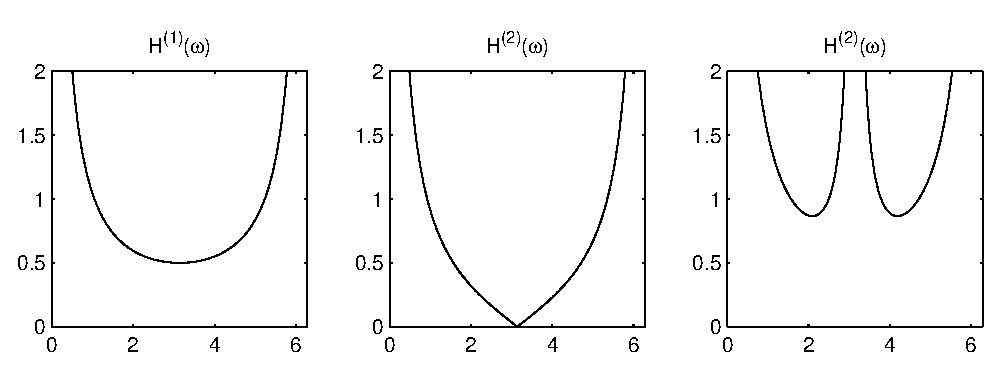
\includegraphics[scale=0.7]{images/meth-quadratures-filtre-recursif.eps}
    \end{center}
    \caption{Frequency responses of the three filters}
              \label{fig-meth-quadratures-recursive-filter}
\end{figure}
\end{correction}
 
 
\begin{correction}{exo-calcul-spline-iir}
\begin{enumerate}
\item We have
\begin{equation*}
\beta^3 (x) = \left\{\begin{array}{ll} 2/3- | x |^2 + | x |^3/2 & \text{si} \; 0 \leq | x | \leq 1, \\(2- | x |)^3/6 & \text{si} \; 1 \leq | x | \leq 2, \\0 & \text{otherwise,} \end{array} \right.
\end{equation*}
which gives $ \beta_d^3 = \{\ldots, \, 0, \, 1/6, \, 2/3, \, 1/6, \, 0, \, \ldots\} $.
\item \index{Decomposition!into simple elements} \index{Simple element} We have the decomposition
\begin{equation*}
\Zz (\Phi_d^3) (z) = \frac{-6 \alpha}{1- \alpha^2} \left(\frac{1}{1- \alpha z^{-1}} + \frac{1}{1+ \alpha z}-1 \right) \quad \text{with} \quad \alpha = \sqrt{3} -2.
\end{equation*}
The fraction in $ z^{-1} $ (respectively in $ z $) corresponds to a recursive causal filter (respectively anti-causal) which is stable. To calculate $ c $, we must filter $ u_d $ by the two filters, (one according to the increasing indices and the other according to the decreasing indices), add the results, subtract $ u_d $, and multiply the whole by $ -6 \alpha/(1- \alpha^2) $.
\item With the previous question, there comes $ b_0 = -6 \alpha/(1- \alpha^2) $ and $ b_1 = \alpha $. We can impose $ c^+ [0] = c^- [K-1] = $ 0. For more complex conditions, we will look at \cite{unser-spline}. The \Matlab{} \ref{listing-spline-1} procedure calculates the coefficients of the interpolation by this method.

\begin{listing} 
\begin{footnotesize}
{\upshape
\begin{tabular}{l} \texttt{\pfunction c = coef\_spline\_1 (ud)} \\
\texttt{K = length(ud); alpha = sqrt(3)-2;} \\
\texttt{b1 = alpha; b0 = -6 * b1/(1-b1{\hatverb}2);} \\
\texttt{c1 = zeros(K, 1); c2 = zeros(K, 1);} \\
\texttt{\pfor i = 2:K} \\
\quad \texttt{c1 (i) = ud(i) + b1 * c1 (i-1);} \\
\texttt{\pend} \\
\texttt{\pfor i = (K-1):-1:1} \\
\quad \texttt{c2 (i) = ud (i) + b1 * c2 (i+1);} \\
\texttt{\pend} \\
\texttt{c = b0 * (c1 + c2-ud);} \\
\end{tabular}
}
\end{footnotesize}
\caption{Procedure \texttt{\upshape coef\_spline\_1}}
\label{listing-spline-1}
\end{listing}
 
\item We have the decomposition
\begin{equation*}
\Zz (\Phi_d^3) (z) = \frac{-6 \alpha}{(1- \alpha z^{-1}) (1- \alpha z)}.
\end{equation*}
The vector $ c $ is therefore obtained by the composition of two filters (one causal, the other anti-causal). The \Matlab{} \ref{listing-spline-2} program uses this second decomposition.

\begin{listing} 
\begin{footnotesize} 
{\upshape
\begin{tabular}{l} \texttt{\pfunction c = coef\_spline\_2 (ud)} \\
\texttt{K = length(ud); alpha = sqrt(3) -2;} \\
\texttt{c = zeros(K, 1); d = zeros(K, 1);} \\
\texttt{\pfor i = 2:K} \\
\quad \texttt{d (i) = 6 * ud (i) -alpha * d (i-1);} \\
\texttt{\pend} \\
\texttt{c (K) = -6 * alpha/(1-alpha{\hatverb}2) * (2*d (K) -6 * ud (K));} \\
\texttt{\pfor i = (K-1):-1:1} \\
\quad \texttt{c (i) = alpha * (c (i+1) -d (i+1));} \\
\texttt{\pend} \\
\end{tabular}
}
\end{footnotesize}
\caption{Procedure \texttt{\upshape coef\_spline\_2}}
\label{listing-spline-2}
\end{listing}
\end{enumerate}
\end{correction}
 
 
\begin{correction}{exo-chirp-transform-finis-corps}
\index{Cooley-Tukey@\nompropreindex{Cooley-Tukey}} Using the fact that $ a \mapsto g^a $ is a bijection of $ \{0, \ldots, \, p-2\} $ into $ \FF_p^* $, we get
\begin{equation*}
\wh{f} (g^{- b}) = f(0) + \sum_{x \in \FF_p^*}{f(x) \omega_p^{- xg^{- b}}} = f(0) + \sum_{a = 0}^{p-2}{f(g^a) \omega_p^{-g^{ab}}}.
\end{equation*}
\index{Translation} \index{Convolution!circular} We denote by $ \wt{f} $ and $ \wt{h} $ the vectors of $ \CC^{p-1} $ defined by $ \wt{f}[k] = f(g^{k}) $ and $ \wt{h}[k] = \omega_p^{- g^{- k}} $. We check that the definition of $ \wt{h} $ is independent of a translation of $ k $ by $ p-1 $, so $ \wt{h} $ can be seen as a function $ (p-1) $ -periodic. Consequently, the expression of $ \wh{f} (g^{- b}) $ corresponds well to the circular convolution $ \wt{f} * \wt{h}[b] $. We can therefore calculate a DFT of length $ p $ thanks to a convolution of length $ p-1 $, therefore to 3 DFTs of length $ p-1 $. This is advantageous because $ p $ does not admit a factorization, whereas $ p-1 $ admits one (it is at least divisible by $ 2 $), which allows to use for example the method of Cooley-Tukey, paragraph \ref{sect2-transfo-cooley-tukey}. \\The \Matlab{} \ref{fft-chirp} procedure uses this method. You must provide it with a generator of $ \FF_p^* $ in the \texttt{g} parameter. It uses an auxiliary function \texttt{invmod}, program \ref{listing-invmod} which computes an inverse modulo $ p $.

\begin{listing} 
\begin{footnotesize} 
{\upshape
\begin{tabular}{l} \texttt{\pfunction y = fft\_chirp (x, g)} \\
\texttt{p = length(x); f = zeros(p-1.1); h = zeros(p-1,1);} \\
\texttt{\pfor k = 0:p-2} \\
\quad \texttt{j = mod(g{\hatverb}k, p); jj = invmod(j, p);} \\
\quad \texttt{f(k+1) = x(j+1); h (k+1) = exp(-2i * pi/p * jj);} \\
\texttt{\pend} \\
\texttt{h = ifft(fft(f).*fft(h));} \\
\texttt{y = zeros(p, 1); y(1) = sum(x);} \\
\texttt{\pfor k = 0:p-2} \\
\quad \texttt{j = mod(g{\hatverb}k, p); jj = invmod(j, p);} \\
\quad \texttt{y(dd+1) = x(1) + h (k+1);} \\
\texttt{\pend} \\
\end{tabular}
}
\end{footnotesize}
\caption{Procedure \texttt{\upshape fft\_chirp}}
\label{fft-chirp}
\end{listing}
 
\begin{listing} \begin{footnotesize}
{\upshape
\begin{tabular}{l} \texttt{\pfunction y = invmod(x, p)} \\
\texttt{[u, y, d] = gcd(x, p); y = mod(y, p);} \\
\end{tabular}
}
 \end{footnotesize}
\caption{Procedure \texttt{\upshape invmod}}
\label{listing-invmod}
\end{listing}
\end{correction}
 
 
\begin{correction}{exo-calcul-approaches-transfo-frac}
\begin{enumerate}
\item We have
\begin{equation*}
\wh{f} (y_k) \approx \frac{a}{N} \sum_{s = 0}^{N-1}{f(x_s) e^{- \imath x_s y_k}} = \frac{a}{N} e^{\imath \delta} \sum_{s = 0}^{N-1}{\wt{f}[s] e^{- \frac{2 \imath \pi}{N} sk \gamma}} = \frac{a}{N} e^{\imath \delta} G (\wt{f}, \, \gamma) [k],
\end{equation*}
where $ \delta = \frac{N}{2} \left(\zeta - \frac{2 \pi}{a} \gamma \frac{N}{2} \right) $ and $ \wt{f}[s] = f [s] e^{- \imath \zeta s} $. If $ \zeta = \frac{p}{q} $, we have
\begin{equation*}
G (\wt{f}, \, \gamma) = \sum_{k = 0}^{N-1}{\wt{f}[s] e^{- \frac{2 \imath \pi}{q N} s (pk)}}.
\end{equation*}
This can be calculated by adding $ N (q-1) $ zeros to the end of $ f $, then calculating a DFT of size $ N q $. The use of the fractional Fourier transform is very advantageous if $ q $ is large.
\item We will define a fractional Fourier transform $ G_{\text{sim}} $ which uses the Simpson method instead of the rectangle method for the Fourier integral. We suppose that $ N = 2 N_0+1 $, and taking care to divide the sums well, we obtain
\begin{align*}
G_{\text{sim}} (f, \, \gamma) [k] & = \frac{1}{3} \sum_{s = 0}^{N_0-1}{f [2s] \omega_N^{-2 sk \gamma}} + \frac{4}{3} \sum_{s = 0}^{N_0-1}{f [2s+1] \omega_N^{- (2s+1) k \gamma}} \\
& + \frac{1}{3} \sum_{s = 1}^{N_0}{f [2s] \omega_N^{- 2 sk \gamma}} = G (g, \, \gamma),
\end{align*}
where $ g $ is defined by $ g [0] = \frac{1}{3} f [0] $, $ g [N-1] = \frac{1}{3} f [N-1] $ and
\begin{equation*}
\left\{\begin{array}{ll} g [2k] = \frac{2}{3} f [2k] & \text{for} \; k = 1, \ldots, \, N_0-1, \\g [2k+1] = \frac{4}{3} f [2k+1] & \text{for} \; k = 0, \ldots, \, N_0-1. \end{array} \right.
\end{equation*}
The \Matlab{} \ref{listing-czt-simpson} procedure uses this method. To calculate $ G_{\text{sim}} (f, \, \gamma) $, it must be called with the parameter \texttt{alpha} equal to $ (\omega_N)^{\gamma} $.

\begin{listing} \begin{footnotesize}
{\upshape
\begin{tabular}{l} \texttt{\pfunction y = czt\_simpson(x, alpha)} \\
\texttt{N = length(x); N0 = (N-1)/2; y = zeros(N, 1);} \\
\texttt{y(1) = x(1)/3; y(N) = x(N)/3;} \\
\texttt{y(2*(1:(N0-1))+1) = 2/3 * x(2*(1:(N0-1))+1);} \\
\texttt{y(2*(0:(N0-1)) + 2) = 4/3 * x(2*(0:(N0-1)) + 2);} \\
\texttt{y = czt(y, alpha);} \\
\end{tabular}
}
\end{footnotesize}
\caption{Procedure \texttt{\upshape czt\_simpson}}
\label{listing-czt-simpson}
\end{listing}
\end{enumerate}
\end{correction}
 
 
\begin{correction}{exo-transforme-fourier-fractionionnaire-2d}
The \Matlab{} \ref{listing-frft} procedure performs the fractional Fourier transform $ G (f, \, \alpha) $, quite simply by using the \texttt{czt} algorithm (\ref{listing-czt}). We can then apply it to the rows and then the columns of a matrix to calculate a 2D transform, as the \ref{listing-frft2d} procedure does.

\begin{listing} \begin{footnotesize}
{\upshape
\begin{tabular}{l} \texttt{\pfunction y = frft (x, alpha)} \\
\texttt{N = length(x);} \\
\texttt{w = exp(-2i * pi * alpha/N);} \\
\texttt{y = czt(x, w);} \\
\end{tabular}
} 
\end{footnotesize}
\caption{Procedure \texttt{\upshape frft}}
\label{listing-frft}
\end{listing}
 
\begin{listing} \begin{footnotesize}
{\upshape
\begin{tabular}{l} \texttt{\pfunction y = frft2d (x, alpha)} \\
\texttt{n = length(x);} \\
\texttt{\pfor i = 1:n} \\
\quad \texttt{y(i,:) = frft (x(i,:), alpha);} \\
\texttt{\pend} \\
\texttt{\pfor j = 1:n} \\
\quad \texttt{y(:,j) = frft (y(:,j), alpha);} \\
\texttt{\pend} \\
\end{tabular}
}
\end{footnotesize}
\caption{Procedure \texttt{\upshape frft2d}}
\label{listing-frft2d}
\end{listing}
\end{correction}

%%%%%%%%%%%%%%%%%%%%%%%%%%%%%%%%%%%%%%%%%%%%%%%%%%%%%%%%
%%%%%%%%%%%%%%%%%%%%%%%%%%%%%%%%%%%%%%%%%%%%%%%%%%%%%%%%
%%%%%%%%%%%%%%%%%%%%%%%%%%%%%%%%%%%%%%%%%%%%%%%%%%%%%%%%
\section{Correction of the exercises of chapter 6}
 
 
\begin{correction}{exo-calculus-pol-cyclotomic}
The procedure \Maple{} \ref{listing-calcul-pol-cyclo} calculates the first integer such that $ \Phi_n $ has a coefficient equal to $ \pm k $. Be careful, it is very slow.

\begin{listing} 
\begin{footnotesize} 
{\upshape
\begin{tabular}{l} \texttt{CycloCoef := \pproc{} (k)} \\
\quad \texttt{\plocal i, j, P, s:} \\
\quad \texttt{\pfor i \pfrom 0 \pto 10000 \pdo} \\
\quad \quad \texttt{P := cyclotomic (i, X): s := degree (P):} \\
\quad \quad \texttt{\pfor j \pfrom 0 \pto s \pdo} \\
\quad \quad \quad \texttt{\pif abs(coeff(P, X, j)) = k \pthen \preturn{}(i): \pend \pif{}:} \\
\quad \quad \texttt{\pend \pdo{}:} \\
\quad \texttt{\pend \pdo{}:} \\
\texttt{\pend \pproc{}:} \\
\end{tabular}
}
\end{footnotesize}
\caption{Procedure \texttt{\upshape CycloCoef}}
\label{listing-calcul-pol-cyclo}
\end{listing}
\end{correction}
 
 
\begin{correction}{exo-demo-cns-existance-ntt}
\begin{enumerate}
\item \index{Subgroup} A primary root $ \zeta $ on $ \FF_p $ is a primitive root. The group generated by $ \zeta $ is cardinal $ n $, it is a subgroup of $ \FF_p^* $, so $ n | p-1 $.
\item We have $ \PGCD (\zeta, \, p) = 1 $, so $ \PGCD (\zeta, \, p^r) = 1 $, so $ \zeta $ is invertible in $ \ZZ/p^r \ZZ $. As $ \Phi (p^r) = p^{r-1} (p-1) $, we have, with Euler's theorem, $ \zeta^{\Phi (p^r)} = \zeta_0^{p-1} = $ 1.
\item In $ \FF_p $, we have $ \zeta^p = \zeta $, so $ \zeta^s = (\zeta^p)^s = \cdots = (\zeta^{p^{r-1}})^s $. So, like $ s <n \leq p $, $ \zeta_0^s-1 $ is invertible in $ \FF_p $. This means that $ \pgcd (\zeta_0^s-1, \, p) = 1 $, so we have $ \pgcd (\zeta_0^s-1, \, p^r) = 1 $, and $ \zeta_0^s-1 $ is also invertible in $ \ZZ/p^r \ZZ $.
\item With the Chinese theorem, we have $ \ZZ/m \ZZ \simeq \prod{\ZZ/p_i^{k_i} \ZZ} $. In each $ \ZZ/p_i^{k_i} \ZZ $, we choose a root \ordin{n}{ième} principal $ \zeta_i $. We then check that $ (\zeta_1, \ldots, \, \zeta_r) \in \prod{\ZZ/p_i^{k_i} \ZZ} $ is a main \ordin{n}{ième} root.
\end{enumerate}
\end{correction}
 
 
\begin{correction}{exo-root-square-primitive}
\begin{enumerate}
\item \index{Divisor of zero} If $ \zeta $ is a \ordin{mn}{th} root of the unit, then $ \alpha = \zeta^m $ is a \ordin{n}{th root} of the unit. Moreover, $ \alpha^i-1 = \zeta^{mi}-1 $ is not a divisor of zero, since $ 0 <mi \leq mn $. Ditto for $ \beta = \zeta^n $. \\Conversely, if $ \zeta^m $ is a principal root \ordin{n}{ième}, then $ \zeta^{mn} = (\zeta^m )^n = 1 $ so $ \zeta $ is a \ordin{mn}{th} root of the unit. Let $ 0 <i <mn $, and $ a $ such that $ a \zeta^i = a $. Let us show that $ a = 0 $. By Euclidean division, we write $ i = nq + r $, with $ 0 \leq r <n $, and $ q <m $. If $ r = 0 $, then, since $ \zeta^{nq}-1 $ is not a divisor of zero (since $ \zeta^m $ is principal root \ordin{n}{th}), we have finished. If $ r> 0 $, then we have, by iterating $ a \zeta^i = a $, the relation $ a (\zeta^i)^k = a $. By taking $ k = m $, we get $ a \zeta^{mnq + mr} = a \zeta^{mr} = a $, which implies $ a = 0 $ because $ \zeta^m $ is principal root \ordin{n}{ième}.
\item The square roots of the unit are roots of the polynomial $ (X-1) (X+1) $ therefore are $ -1 $ or $+1 $. To obtain a principal root, it is therefore necessary that $ \zeta = -1 $ and that $ \zeta-1 = -2 $ is not a divisor of zero. So if $ 2 $ is not a divisor of zero, $ -1 $ is the only principal square root.
\item The property was demonstrated in the previous question for $ k = 1 $. We assume the property demonstrated up to the range $ k-1> 0 $. With question 1, $ \zeta $ is a \ordin{(2^k)}{ith} principal root if and only if \ordin{(2^{k-1})}{ième} is a principal square root (thus equal to $ -1 $) and if $ \zeta^2 $ is a root \ordin{(2^{k-1})}{th}. By applying the induction hypothesis to $ \zeta^2 $, we have $ (\zeta^2)^{2^{k-2}} = \zeta^{2^{k-1}} = -1 $.
\end{enumerate}
\end{correction}
 
 
\begin{correction}{exo-boolean-functions}
\begin{enumerate}
\item We denote by $ v_k^0 = 1 + v_k $ and $ v_k^1 = v_k $. We have decomposition
\begin{equation*}
\wt{f} (v_0, \ldots, \, v_{n-1}) = \sum_{(i_0, \ldots, \, i_{n-1}) \in \{0, \, 1\}^n}{\wt{f} (i_0, \ldots, \, i_{n-1}) \prod_{k = 0}^{n-1}{v_k^{i_k}}}.
\end{equation*}
By developing the products, we find a polynomial of the requested form. Since there are $ 2^n $ such polynomials, and $ 2^n $ boolean functions, the decomposition found is unique.
\item We have
\begin{equation*}
\Ww (f) (k) = \sum_{u \in (\FF_2)^n}{(-1)^{\dotp{u}{k} + \wt{f} (u)}},
\end{equation*}
so $ \Ww (f) (k) $ is equal to the number of $ 0 $ minus the number of $ 1 $ in the vector $ \{\wt{f} (u) + \dotp{u}{k}\}_{u \in (\FF_2)^n} $. This means that
\begin{equation*}
\Ww (f) (k) = 2^n - 2 d (f, \, f_{k, \, 0}).
\end{equation*}
As we also have
\begin{equation*}
d (f, \, 1 + f_{k, \, 0}) = d (f, \, f_{k, \, 1}) = 2^n - d (f, \, f_{k, \, 0}),
\end{equation*}
he comes
\begin{equation*}
\min \left(d (f, \, f_{k, \, 0}), \, d (f, \, f_{k, \, 1}) \right) = \frac{1}{2} \left(2^n - | \Ww (f) (k) | \right).
\end{equation*}
Hence the result, passing to min on the set of $ f_{k, \, b} $.
\item If $ f $ matches $ | \Ww (f) (k) | = 2^{n/2} $, then $ N (f) = 2^{n-1} -2^{n/2-1} $. Let $ g $ be a function such that $ \exists k, \; | \Ww (g) (k) | \neq 2^{n/2} $. With the Plancherel formula, proposition \ref{prop-formula-floorel}, we have
\begin{equation*}
\sum_{s = 0}^{2^n-1}{| \Ww (g) (s) |^2} = 2^{2n}.
\end{equation*}
Thus, since there are $ 2^n $ terms in the sum, $ \exists k $ such that $ | \Ww (g) (k) | > 2^{n/2} $. So we have $ N (g) <2^{n-1} -2^{n/2-1} $.
\item \index{Function!bent} \index{Bent} We have
\begin{align*}
\Ww (h) (w) & = \sum_{t \in (\FF_2)^{n + m}}{(-1)^{\dotp{w}{t} + \wt{h} (t )}} \\
& = \sum_{r \in (\FF_2)^{n}}{\sum_{s \in (\FF_2)^{m}}{(-1)^{\dotp{u}{r} + \wt{f} (r)} (-1)^{\dotp{v}{s} + \wt{g} (s)}}} = \Ww (f) (u) \Ww (g) (v ).
\end{align*}
If $ \wt{f} $ and $ \wt{g} $ are bents, $ | \Ww (f) (u) | = 2^{n/2} $ and $ | \Ww (g) (v) | = 2^{m/2} $ and therefore we have $ | \Ww (h) (w) | = 2^{(m + n)/2} $. Conversely, if for example $ \wt{f} $ is not bent, we have already seen in question 3 that $ \exists u_0, \; | \Ww (f) (u_0) | > 2^{n/2} $. If we assume that $ \wt{h} $ is bent, then for $ w = (u_0, \, v) $,
\begin{equation*}
2^{(m + n)/2} = | \Ww (h) (w) | = | \Ww (f) (u_0) | | \Ww (g) (v) | \Longrightarrow \forall v, \; | \Ww (g) (v) | <2^{m/2},
\end{equation*}
which is impossible because $ N (g) \leq 2^{m-1} - 2^{m/2-1} $. \\We check that $ \Ww (f_0) = \{2, \, 2 , \, 2, \, - 2\} $, so $ f_0 $ is bent. Thus the function
\begin{equation*}
f(u_0, \ldots, \, u_{n-1}) = u_0 u_1 + \cdots + u_{n-2} u_{n-1}
\end{equation*}
is bent.
\item The dimension of $ R (1, \, n) $ is $ n+1 $, and its minimum distance is $ 2^{n-1} $. This is because the functions $ \wt{f}_{a, \, b} $, for $ a \neq 0 $, take $ 2^{n-1} $ times the value $ 0 $, and $ 2^{n-1} $ times the value $ 1 $. \\We have $ f_{a, \, b} (u) = (-1)^b \Ww (\delta_a) (u) $, which is calculated quickly using the FWT algorithm. The \Matlab{} \ref{listing-encode-rm} procedure performs this encoding. It takes as parameter $ a $ as an integer $ 0 \leq a \leq 2^n-1 $. 

\begin{listing} 
\begin{footnotesize}
{\upshape
\begin{tabular}{l} \texttt{\pfunction y = encode\_rm(a, b, n)} \\
\texttt{y = zeros(2{\hatverb}n, 1); y(a+1) = 1;} \\
\texttt{y = fwt(y); y = (1-y)/2;} \\
\texttt{\pif{} (b==1) y = 1-y; \pend{};} \\
\end{tabular}
}
\end{footnotesize}
\caption{Procedure \texttt{\upshape encode\_rm}}
\label{listing-encode-rm}
\end{listing}

With question 2, we see that $ d (F_{a, \, b}, \, F) $ is minimal when $ | \Ww (f) (a) | $ is maximum. Then, we have $ b = 0 $ if $ \Ww (f) (a)> 0 $, and $ b = 1 $ otherwise. The \Matlab{} \ref{listing-decode-rm} procedure performs this decoding, and takes as input a vector \texttt{x} of size $ 2^n $ representing $ F $.

\begin{listing} 
\begin{footnotesize}
 {\upshape
\begin{tabular}{l} \texttt{\pfunction y = decode\_rm(x)} \\
\texttt{N = length(x);} \\
\texttt{f = fwt((-1).{\hatverb}x);} \\
\texttt{[v, a] = max(abs(f));} \\
\texttt{y = encode\_rm(a-1, f(a) <0, log2(N));} \\
\end{tabular}
}
\end{footnotesize}
\caption{Procedure \texttt{\upshape decode\_rm}}
\label{listing-decode-rm}
\end{listing}

\end{enumerate}
\end{correction}
 
 
\begin{correction}{exo-learning-boolean-functions}
\begin{enumerate}
\item We have, using Plancherel's formula, proposition \ref{prop-formula-floorel},
\begin{equation*}
E ((fh)^2) = \sum_{\alpha \neq \beta}{a_\alpha^2} = 1-a_\beta^2.
\end{equation*}
 
\item We denote by $ I (x) $ the function which is worth $ 1 $ if $ f(x) \neq h_0 (x) $, and $ 0 $ otherwise. We have
\begin{equation*}
\PP (f(x) \neq h_0 (x)) = \frac{1}{2^n} \sum_{x}{I (x)}.
\end{equation*}
We must therefore show that $ I (x) \leq (f(x) -h (x))^2 $. If $ f(x) \neq h_0 (x) $, then $ I (x) = 0 $ and the inequality is true. Otherwise, then necessarily $ | f(x) -h (x) | \geq 1 $, and we have $ I (x) = 1 \leq (f(x) -h (x))^2 $.
\item By applying the Chernoff-Hoeffding bound to $ X_i = f(x_i) $, which are iid and such that $ E (X_i) = E (f) $, $ X_i \in [-1, \, 1] $, we get
\begin{equation*}
\PP (| \wt{c_\beta} - c_\beta | \geq \lambda) \leq 2e^{- \lambda^2 m/2} \leq \delta.
\end{equation*}
With a probability less than $ \delta $, we therefore have
\begin{equation*}
\PP (f(x) \neq \varphi_0 (x)) \leq E ((f- \wt{a_\beta} \chi_\beta)^2) \leq \sum_{\alpha \neq \beta}{a_\alpha^2} + (a_\beta- \wt{a_\beta})^2 \leq 1-a_\beta^2 + \lambda^2.
\end{equation*}
 
\item We note $ S_d \eqdef \enscond{s}{w (s) <d} $. Using the Chernoff-Hoeffding bound, we have $ \PP (| a_s- \wt{a_s} | \geq \lambda) \leq 2e^{- \lambda^2 m/2} $. Moreover, under the condition $ | a_s- \wt{a_s} | \leq \lambda $, we have
\begin{equation*}
E ((f- \varphi)^2) \leq \alpha + \sum_{s \in S_d}{(a_s - \wt{a_s})^2} \leq \alpha + n^d \lambda^2,
\end{equation*}
since $ \Card (S_d) \leq n^d $. To have $ \PP (f(x) \neq \varphi (x)) \leq \alpha + \epsilon $, we must therefore impose $ \lambda \leq \sqrt{\epsilon/n^d} $, and so that this takes place with a probability $ 1- \delta $, we must have $ 2 e^{- \lambda^2 m/2} n^d \leq \delta $, since
\begin{equation*}
\PP \left(\forall s \in S_d, \; | a_s - \wt{a_s} | \geq \lambda \right) \leq \sum_{s \in S_d}{\PP (| a_s - \wt{a_s} | \geq \lambda)} \leq 2 e^{- \lambda^2 m/2} n^d.
\end{equation*}
\end{enumerate}
\end{correction}
 
 
\begin{correction}{exo-matrices-generator-control}
\begin{enumerate}
\item We denote by $ G $ and $ H $ generator and control matrices. We have
\begin{equation*}
y \in \Cc^\bot \Leftrightarrow \forall x \in (\FF_p)^n, \; \dotp{G x}{y} = 0 \Leftrightarrow \forall x \in (\FF_p)^n, \; \dotp{x}{\transp{G} y} = 0 \Leftrightarrow \transp{G} y = 0.
\end{equation*}
So a control matrix of $ \Cc^\bot $ is $ \transp{G} $, and a generator matrix is $ \transp{H} $.
\item Such a form simplifies the encoding (as well as the decoding, as we will see on the form of $ H $). We can choose $ H = (A | \Id_{nm}) $, and we verify that $ HG = 0 $, with $ \text{rang} (G) = mn $.
\item Two codes are equivalent if we can pass from a $ G_1 $ matrix of the first code to a $ G_2 $ matrix of the second by \begin{rs}
\item \index{Elementary operations} elementary operations on the columns (which do not modify the space generated by the columns, and therefore the code). This corresponds to the operations $ C_i \leftarrow \lambda C_i $ as well as $ C_i \leftarrow C_i + \lambda C_j $, for $ C_i \neq C_j $ of columns and $ \lambda \neq 0 $.
\item permutation of lines (which corresponds to a permutation of symbols).
\end{rs} \index{Gauss@\nompropreindex{Gauss}} By Gaussian pivoting (see \cite{ciarlet}), we can reduce ourselves, by these operations, to a systematic form.
\end{enumerate}
\end{correction}
 
 
\begin{correction}{exo-codes-hamming}
\begin{enumerate}
\item \index{Syndrome} \index{Decoding} The minimum distance of a code is the minimum number of linearly dependent columns. As two columns are distinct here, their modulo 2 sum is never zero, and they are therefore independent. On the other hand, this sum is necessarily equal to a third column, so we can find three related columns. The minimum distance is therefore 3. \\Since $ H $ has $ k $ lines, the dimension of $ \Cc $ is $ 2^k-1-k $. If $ v'= v + e $ is the word received, with $ w (e) = 1 $ and $ v \in \Cc $, then $ s = H v' = H e $ is the syndrome. So, $ s $ is a column of $ H $. For example, if we have taken as \ordin{i}{th} column of $ H $ the decomposition of $ i $ into binary, then the position of the error in $ v'$ is simply the integer of which $ s $ is the binary decomposition. The \Matlab{} \ref{listing-decodage-hamming} function performs the decoding. It uses the procedure \texttt{writing\_binary} \ref{binary-writing-listing}, which decomposes an integer into binary writing.

\begin{listing} \begin{footnotesize}
{\upshape
\begin{tabular}{l} \texttt{\pfunction y = decode\_hamming (x)} \\
\texttt{n = length(x); k = log2(n+1);} \\
\texttt{H = zeros(k, n); y = x;} \\
\texttt{\pfor{}(j = 1:n) H(:,j) = write\_binary(j, k); \pend{};} \\
\texttt{s = mod(H * x, 2);} \\
\texttt{e = dot (s, 2.{\hatverb}(0:(k-1)));} \\
\texttt{\pif{} (e $ \sim $ = 0) y(e) = 1-y(e); \pend{};} \\
\end{tabular}
}
\end{footnotesize}
\caption{Procedure \texttt{\upshape decode\_hamming}}
\label{listing-decodage-hamming}
\end{listing}
 
\begin{listing} \begin{footnotesize}
{\upshape
\begin{tabular}{l} \texttt{\pfunction y = write\_binary(x, k)} \\
\texttt{y = zeros(k, 1);} \\
\texttt{\pfor{}(i = 1:k) q = floor(x/2); y(i) = x-2*q; x = q; \pend{};} \\
\end{tabular}
}
\end{footnotesize}
\caption{Procedure \texttt{\upshape write\_binary}}
\label{binary-writing-listing}
\end{listing}
 
\item In base $ \{\alpha, \ldots, \, \alpha^{k}\} $ of $ \FF_{2^k} $ as vector space on $ \FF_2 $, $ \alpha $ s' written, in vector form, $ (1, \, 0, \ldots, \, 0) $, $ \alpha^2 $ is written $ (0, \, 1 ,, \, 0, \ldots, \, 0) $, etc. The $ \alpha^i $, for $ i $ between $ 1 $ and $ n $, describe all binary representations of numbers between $ 1 $ and $ n $. A word of $ \Cc_\alpha $, the BCH code generated by $ \alpha $ (of assigned distance $ n $) is represented by a polynomial $ P $ and $ P \in \CC_\alpha $ if and only if $ P (\alpha) = \cdots = P (\alpha^{n}) = $ 0. By writing $ P $ in the form of a binary vector $ \wt{P} $ of size $ n $, the preceding equalities are written $ H \wt{P} = 0 $. This code is therefore the Hamming code of size $ n $.
\item There are $ n+1 = 2^k $ words in a ball of radius 1. Since the minimum code distance is 3, the balls centered in the code words are disjoint. This set of balls therefore contains $ 2^m \times 2^k = 2^{2^k-1} = 2^n $ words, that is to say all the space $ (\FF_2)^n $ . In the case of $ n = 7 $, we can take
\begin{equation*}
H = \begin{pmatrix} 1 & 0 & 1 & 0 & 1 & 0 & 1 \\0 & 1 & 1 & 0 & 0 & 1 & 1 \\0 & 0 & 0 & 1 & 1 & 1 & 1 \end{pmatrix},
\end{equation*}
and we check that $ HG = 0 $, where $ G $ is the matrix of the example \ref{exmp-code-hamming-7}.
\item \index{Word weight} The generator matrix of $ \Cc^\bot $ is $ G_0 = \transp{H} $. For $ H $, we have chosen for \ordin{i}{ième} column ($ 1 \leq i \leq 2^k-1 $) the decomposition of $ i $ in binary writing. We precede $ G_0 $ with a line of 0 (which does not change the weight of the words). We then see that the first column is an alternation of $ 0 $ and $ 1 $, that the second is an alternation of $ 00 $ and $ 11 $, and so on. All the columns of $ G_0 $ thus have for weight $ 2^{k-1} $. We can easily see that an elementary operation on the rows of the type $ L_i \leftarrow L_i + \sum_{j \in J}{L_j} $ is content to perform a permutation on the columns of the matrix, therefore the weight of the columns remainder $ 2^{k-1} $. By such operations, we obtain all the non-zero words of $ \Cc^\bot $, which therefore have as weight $ 2^{k-1} $. As the distance between two words is the weight of the word difference, this code is very simple.
\item \index{Space!projective} On $ \FF_q $, we choose for the columns of $ H $ representatives of vector lines, i.e. of the projective space $ \PP (\FF_q^n ) $. As $ \Card (\PP (\FF_q^n)) = \frac{q^k-1}{q-1} $ (each line has $ q-1 $ non-zero elements), we get the size and the desired dimension. The proof of the minimum distance is unchanged. The code is still perfect, a ball of radius 1 containing $ n (q-1)+1 $ words.
\end{enumerate}
\end{correction}
 
 
\begin{correction}{exo-pol-enumerateur-hamming}
\begin{enumerate}
\item The binary representation of integers allows to establish a bijection between the set $ \{1, \ldots, \, 2^k-1\} $ and $ \FF_2^k \backslash \{0\} $. For $ k = $ 3, we have
\begin{equation*}
W_{\Cc_7} (X, \, Y) = X^7 + 7 X^3Y^4 + 7 X^4 Y^3 + X^7
\end{equation*}
 
\item See exercise \oldref{exo-codes-hamming}, question 4.
\item We have $ W_{\Cc^\bot} (X, \, Y) = Y^n + 2^{k-1} X^{n-2^{k-1}} Y^{2^{k-1}} $, hence the result with the theorem \ref{thm-id-mac-williams-correctors-codes}.
\item We denote by $ P (Y) = W_\Cc (1, \, Y) $. We have $ A_s = \frac{1}{s!} \frac{\d^s P}{\d Y^s} (0) $. The script \Maple{} \ref{listing-repartition-hamming} performs the calculation, and we find $ A_1 = A_2 = 0 $, which is logical, since the minimum distance is 3. Here are some values of $ A_k $
\begin{equation*}
\begin{array}{c || c | c | c | c | c | c} k & 1 & 2 & 3 & 4 & 5 & 6 \\\hline A_k & 0 & 0 & \frac{n (n -1)}{6} & \frac{n (n-1) (n-3)}{24} & \frac{n (n-1) (n-3) (n-7)}{120} & \frac{n (n-1) (n-3) (n-5) (n-7)}{720} \end{array}
\end{equation*}
 
\begin{listing} 
\begin{footnotesize} 
{\upshape
\begin{tabular}{l} \texttt{P := Y -> 1/(n+1) * ((1 + Y){\hatverb}n + n * (1-Y){\hatverb}(( n+1)/2) * (1+Y){\hatverb}((n-1)/2));} \\
\texttt{A := s -> factor (1/(s!) * eval(diff(P (Y), Y\$s), Y=0));} \\
\end{tabular}
}
\end{footnotesize}
\caption{Calculation of $ A_k $ for a Hamming code}
\label{listing-repartition-hamming}
\end{listing}
 
\item To show symmetry, we have to show that $ P (Y) = Y^n P (1/Y) $, which is easily verified.
\end{enumerate}
\end{correction}
 
 
\begin{correction}{exo-code-hamming-extended}
We check that $ W_\Cc (X, \, Y) = X^8+14 X^4 Y^4 + Y^8 $, and that this polynomial is invariant by the change of variable $ (X, \, Y ) \mapsto \frac{1}{\sqrt{2}} (X + Y, \, XY) $ (this can easily be checked using \Maple{}).
\end{correction}
 
 
\begin{correction}{exo-code-repetition}
\begin{enumerate}
\item $ \Cc $ is a code of dimension $ 1 $ and minimum distance $ n $. Its enumerator polynomial is $ Y^n + (q-1) X^n $.
\item \index{Parity bit} \index{Code!dual} \index{Dual!of a code} We have $ x \in \Cc^\bot \Leftrightarrow \sum{x_i} = 0 $ in $ \FF_q $. The dual code corresponds to the code of the parity bit (example \ref{exmp-bit-parite} which we extend to $ \FF_q $). It has dimension $ n-1 $ and minimum distance $ 1 $. We can easily see that $ \Cc = \Cc^\bot $ if and only if $ n = 1 $ (trivial code) or $ n = 2 $.
\end{enumerate}
\end{correction}
 
 
\begin{correction}{exo-codes-hadamard}
\begin{enumerate}
\item \index{Code!of Reed-Muller} \index{Reed-Muller@\nompropreindex{Reed-Muller}} \index{Non-linearity} In the case of the construction by Walsh matrix ($ n = 2^k $), the words of $ \Aa_n $ are the words of $ R (1, \, k) $, the Reed-Muller code (see exercise \oldref{exo-boolean-functions}, question 5), to which the first symbol has been removed. Equivalently, $ R (1, \, k) $ corresponds to the code $ \Aa_n $ with an additional parity bit (which is always 1). For this construction, $ \Aa_n $, just like $ \Bb_n $, is therefore linear. For $ n = 12 $, with the construction of Paley, we obtain the following code $ \Bb_{12} $, which is non-linear.
\begin{equation*}
\begin{array}{c | c} \Aa_{12} & \Bb_{12} \backslash \Aa_{12} \\\hline \\[- 3mm] (00000000000) \; (00010110111) & (11111111111) \; (11101001000) \\[1mm] (11011100010) \; (10001011011) & (00100011101) \; (01110100100) \\[1mm] (01101110001) \; (11000101101) & (10010001110) \; (00111010010) \\[1mm] (10110111000) \; (11100010110) & (01001000111) \; (00011101001) \\[1mm] (01011011100) \; (01110001011) & (10100100011) \; (10001110100) \\[1mm] (00101101110) \; (10111000101) & (11010010001) \; (01000111010) \end{array}
\end{equation*}
 
\item The orthogonality of the lines of $ H_n $ means exactly that two lines have as many equal entries as there are different entries. Two words of $ \Aa_n $ are therefore distant by $ n/2 $, which is the minimum distance. If we denote by $ u, \, v \in \Aa_n $ and $ \ol{u}, \, \ol{v} $ their complements, we have $ d (u, \, v) = d (\ol{u}, \, \ol{v}) = n/2 $, and $ d (u, \, \ol{v}) = n/2-1 $. So the minimum distance of $ \Bb_n $ is $ n/2-1 $. The code $ \Aa_n $ is of size $ n-1 $ with $ n $ elements, and $ \Bb_n $ is of size $ n-1 $ with $ 2n $ elements.
\end{enumerate}
\end{correction}
 
 
\begin{correction}{exo-polynomials-mds}
\begin{enumerate}
\item By developing the equality of MacWilliams, we get
\begin{equation*}
| \Cc | W_{\Cc^\bot} (1, \, Y) = \sum_{k = 0}^n{A_k \left(\sum_{j = 0}^{nk}{C_{nk}^j Y^j} \right) \left(\sum_{j = 0}^{k}{(- 1)^jC_{k}^j Y^j} \right)}.
\end{equation*}
By equaling the coefficients of these two polynomials, we find the required equalities.
\item We derive $ k $ times the equality $ 2^{nm} \Ww_{\Cc} (X, \, 1) = \Ww_{\Cc^\bot} (X+1, \, X-1) $. By using Leibniz's rule to derive a product, we get
\begin{equation*}
2^{nm} \sum_{i = 0}^{nk}{A_i k!C_{ni}^k X^i} = \sum_{i = 0}^k{A_i'\sum_{s = 0}^k{C_k^s \frac{\d^{ks}}{\d X^{kz}} (X+1)^{ni} \frac{\d^s}{\d X^s} (X-1)^i}}.
\end{equation*}
By making $ X = 1 $ in this equality, only the term corresponding to $ s = i $ remains in the second sum from the right. We obtain the desired equalities.
\item There is no word of weight $ i \in \{1, \ldots, \, d-1 = nm\} $ in $ \Cc $. For $ \Cc^\bot $, we must show that its minimum distance is $ m+1 $. Indeed, $ d $ is equal to the smallest number of linearly dependent columns in $ H $ (a control matrix of $ \Cc $). So the greatest number of linearly independent columns in $ H $ is equal to $ d-1 = nm $. Now $ \transp{H} $ is the generator matrix of $ \Cc^\bot $, so as soon as a word of $ \Cc^\bot $ has less than $ nk $ non-zero coordinates, this word is zero. As a result, the minimum distance of $ \Cc^\bot $ is at least $ n- (nk) +1 = k+1 $. There is in fact equality by applying the Singleton bound to $ \Cc^\bot $. By restricting the sums to indices $ i $ such as $ A_i \neq 0 $ and $ A_i'\neq 0 $, using $ C_{n}^{nk} = C_n^k $, and $ A_0' = 1 $ , we obtain the requested $ m $ equations.
\item We have a system of $ m $ equations with $ m $ unknowns (the $ A_i $, for $ i = n-m+1, \ldots, \, n $). This system is in fact triangular, and it is easily resolved by ascent. Thus, the $ A_i $ are uniquely determined. For example, for $ i = m-1 $, we have $ A_d = C_n^{k-1} $.
\end{enumerate}
\end{correction}
 
 
\begin{correction}{exo-terminal-linear-programming}
\begin{enumerate}
\item With the proposition \ref{prop-positivite-repartition-duale}, we know that $ B_i'\geq 0 $. With the expression of $ A_i'$ found in exercise \oldref{exo-polynomials-mds}, question 1, which extends to the distribution $ B_i' $ (thanks to the theorem \ref{thm-id-mac-williams-functions}), we get the desired inequalities.
\item If $ \Cc $ has minimum distance $ d $, then $ B_1 = \cdots = B_d = 0 $, and the cardinality of $ \Cc $ is $ \sum_{i = 0}^n{B_i} $ . The distance distribution of $ \Cc $ therefore belongs to $ E_n^d $, and we find the announced bound.
\end{enumerate}
\end{correction}

%%%%%%%%%%%%%%%%%%%%%%%%%%%%%%%%%%%%%%%%%%%%%%%%%%%%%%%%
%%%%%%%%%%%%%%%%%%%%%%%%%%%%%%%%%%%%%%%%%%%%%%%%%%%%%%%%
%%%%%%%%%%%%%%%%%%%%%%%%%%%%%%%%%%%%%%%%%%%%%%%%%%%%%%%%
\section{Correction of the exercises of chapter 7}
 
 
\begin{correction}{exo-reductibility-decomposability}
\index{Sub-representation} The line $ \Vect (e_1) $ is stable, so the representation is reducible. On the other hand, if the representation were decomposable, we would have the sum of sub-representations $ K^2 = \Vect (e_1) \oplus \Vect (e_2 + \lambda e_1) $, where $ \lambda \in K $. It is easy to see that $ \Vect (e_2 + \lambda e_1) $ cannot be stable.
\end{correction}
 
 
\begin{correction}{exo-stationary-operators}
We denote by $ \varphi = A \delta_e $, where $ e $ is the neutral element of $ G $. We have
\begin{equation*}
A f = \sum_{g \in G}{f(g) A \delta_g} = \sum_{g \in G}{f(g) \tau_{g} (A{\delta_e})} = \sum_{g \in G}{f(g) (\tau_g f)} = f * \varphi.
\end{equation*}
\end{correction}
 
 
\begin{correction}{exo-irred-representation-degre-1} \index{Representation!of morphisms} \index{Tensor product} We can see $ \chi_W = \chi_U \chi_V $ as the character of the representation of morphisms on $ W = \Ll (U, \, V^*) $, or as the tensor product $ W = U \otimes V $. As $ U $ is non- trivial, $ \chi_W $ is distinct from $ \chi_U $ and $ \chi_V $, so we have constructed a new representation. As $ | \chi_U | = 1 $, we have
\begin{equation*}
\sum_{g \in G}{| \chi_W (g) |^2} = \sum_{g \in G}{| \chi_V (g) |^2} = |G|,
\end{equation*}
therefore $ W $ is indeed irreducible.
\end{correction}
 
 
\begin{correction}{exo-representation-product}
\index{Product!tensor} We denote by $ \rho_k: G \rightarrow GL (V_k) $, $ k = 1, \ldots, \, p $, the irreducible representations of $ G $, and $ \sigma_l: H \mapsto GL (W_l) $, $ l = 1, \ldots, \, q $, those of $ H $. We denote by $ m_k = \dim (U_k) $ and $ n_l = \dim (V_l) $. For $ (k, \, l) \in \{1, \ldots, \, p\} \times \{1, \ldots, \, q\} $, we define
\begin{equation*}
\tau_{k, \, l} (g, \, h) = \rho_k (g) \otimes \sigma_l (h) \in GL (V_k \otimes W_l),
\end{equation*}
which is a representation of $ G \times H $ over $ V_k \otimes W_l $. We have $ \chi_{\tau_{k, \, l}} = \chi_{\rho_k} \chi_{\sigma_l} $, in particular, $ \norm{\chi_{\tau_{k, \, l}}}_2 = \norm{\chi_{\rho_k}}_2 \norm{\chi_{\sigma_l}}_2 = 1 $, so $ \tau_{k, \, l} $ is irreducible. In addition, we have
\begin{equation*}
\sum_{k, \, l}{\dim (V_k \otimes W_l)^2} = \sum_{k, \, l}{m_k^2 n_l^2} = |G| \times | H | = | G \times H |,
\end{equation*}
therefore we have found all the irreducible representations.
\end{correction}
 
 
\begin{correction}{exo-action-polynomials}
\begin{enumerate}
\item For $ \sigma \in \mathfrak{S}_n $, we consider the matrix $ M_\sigma: e_i \mapsto e_{\sigma (i)} $. The group $ G = \mathfrak{S}_n $ is isomorphic to the matrix group $ H = \{M_\sigma\}_{\sigma \in G} $, and the action of $ \mathfrak{S}_n $ by permutation of the indeterminates corresponds to the linear action of $ H $ on $ K [X_1, \ldots, \, X_n] $. \\A classical result asserts that the ring of invariants is generated by the polynomials
\begin{equation*}
\sigma_k (X_1, \ldots, \, X_n) \eqdef \sum_{i_1 <\cdots <i_k}{X_{i_1} X_{i_2} \cdots X_{i_k}}.
\end{equation*}
 
\item We have $ K [X, \, Y]^{V_4} = K [X^2, \, Y^2] $. Writing an element of $ K [X, \, Y]^{V_4} $ as a function of $ X^2 $ and $ Y^2 $ is unique. \\We have $ K [X, \, Y]^{C_2} = K [X^2, \, Y^2, \, XY] $. The decomposition is not unique, since we have the relation $ (XY)^2 = X^2 Y^2 $.
\item If $ f = \sum{c_\alpha X^\alpha} \in K [X_1, \ldots, \, X_n]^G $, then $ f = \sum{c_\alpha R_G (X^\alpha )} $. Thus, if we prove that $ R_G (X^\alpha) $ is written as a polynomial in $ R_G (X^\beta) $ for $ | \beta | \leq |G| $, we can write $ f $ as a function of these $ R_G (X^\beta) $.
\item \index{Polynomial!symmetric} We have $ (U_A)^k = \sum_{| \alpha | = k}{a_\alpha (A \cdot X)^\alpha u^\alpha} $. By adding these equalities for $ A \in G $, we find the expression of the desired $ S_k = S_k (U_A \;; \; A \in G) $. Any symmetric polynomial in $ U_A $ is written as a function of $ |G| $ Newton sums $ S_1, \ldots, \, S_{|G|} $. Since $ S_k $ is a symmetric polynomial, there exists $ F \in K [Y_1, \ldots, \, Y_{|G|}] $ such that $ S_k = F (S_1, \ldots, \, S_{|G|}) $, which gives the requested polynomial equality. By equaling the coefficients of $ u^\alpha $ of the two members of the equality, we see that $ |G| a_\alpha R_G (X^\alpha) $ is equal to a polynomial in $ R_G (X^\beta) $, for $ | \beta | \leq |G| $. Since $ K $ has characteristic 0, we can divide by $ |G| a_\alpha $.
\item We can calculate the $ R_{C_4} (X^\beta) $, for $ | \beta | \leq $ 4:
\begin{equation*}
\begin{array}{c|c} X^i Y^i & R_{C_4}(X^i Y^i) \\ \hline X & 0 \\ Y & 0 \\ X^2 & (X^2+Y^2)/2 \\ X Y & 0 \\ Y^2 & (X^2+Y^2)/2 \\ X^3 & 0 \\ X^2 Y & 0 \\ \end{array} \quad \quad \begin{array}{c|c} X^i Y^i & R_{C_4}(X^i Y^i) \\ \hline X Y^2 & 0 \\ Y^3 & 0 \\ X^4 & (X^4+Y^4)/2 \\ X^3 Y & (X^3 Y - X Y^3)/2 \\ X^2 Y^2 & X^2 Y^2 \\ X Y^3 & -(X^3 Y - X Y^3)/2 \\ Y^4 & (X^4+Y^4)/2 \\ \end{array}
\end{equation*}
The ring of invariants is therefore generated by
\begin{equation*}
P_1 = X^2 + Y^2, \quad P_2 = X^4 + Y^4, \quad P_3 = X^3 Y - XY^3, \quad P_4 = X^2 Y^2.
\end{equation*}
However, we note that $ P_2 = P_1^2 - 2 P_4 $, so we can remove $ P_2 $ from this list.
\end{enumerate}
\end{correction}
 
 
\begin{correction}{exo-thm-molien}
\begin{enumerate}
\item The action of $ G $ being linear, it preserves the degree of the homogeneous components. Since two polynomials are equal if and only if their homogeneous components are equal, we deduce the desired result.
\item \index{Trace} \index{Reynolds!operator} The theorem \ref{thm-pte-operator-reynolds}, tells us that $ \dim_{\CC} (V_s^G) = \tr (R_G) $, where $ R_G $ is the Reynolds operator for the $ \rho_s $ representation. As $ \tr (R_G) = \frac{1}{|G|} \sum_{g \in G}{\tr (A^{[s]})} $, we obtain the requested formula.
\item Let $ A \in G $, with eigenvalues $ \omega_1, \ldots, \, \omega_n $. With a change of base, we can write
\begin{equation*}
A = A^{[1]} = \diag (\omega_1, \ldots, \, \omega_n), \quad A^{[s]} = \diag (\omega_1^s, \ldots, \, \omega_n^s, \, \omega_1^{s-1} \omega_2, \ldots).
\end{equation*}
So we have
\begin{equation*}
\tr \left(A^{[s]} \right) = \sum_{i_1 \leq \cdots \leq i_s}{\omega_{i_1} \cdots \omega_{i_s}},
\end{equation*}
which corresponds well to the power of $ \lambda^s $ in the expansion of
\begin{equation*}
\det \left(\Id - \lambda A \right)^{-1} = \prod_{i = 1}^n{(1- \lambda \omega_i)^{-1}}.
\end{equation*}
 
\item The group $ G_1 $ has the Molien series $ [(1- \lambda) (1- \lambda^2)]^{-1} $. The group $ G_2 $ has the Molien series $ (1- \lambda^2)^{- 2} $. The number of linearly independent polynomials limits the number of algebraically independent polynomials, which makes it possible to limit the search.
\end{enumerate}
\end{correction}
 
 
\begin{correction}{exo-lemma-cauchy-frobenius}
\begin{enumerate}
\item We have
\begin{equation*}
\dotp{\chi_1}{\chi_\pi} = \frac{1}{|G|} \sum_{g \in G}{| \chi_\pi (g) |} = \frac{1}{|G|} \sum_{g \in G}{| X_g |}.
\end{equation*}
 
\item We denote by $ G_x = \enscond{g \in G}{g \cdot x = x} $ the stabilizer of $ X $, and $ G x = \enscond{g \cdot x}{g \in G} $ the orbit of $ x $. We have $ |G| = | G_x | | G x | $ (see for example \cite{perrin}). We denote by $ x_1, \ldots, \, x_t $ the representatives of $ t $ distinct orbits of the action of $ G $ on $ X $. We denote by $ T = \enscond{(g, \, x) \in G \times X}{g \cdot x = x} $. By counting \guill{in both directions} the elements of $ T $, we have
\begin{equation*}
\sum_{g \in G}{| X_g |} = | T | = \sum_{x \in X}{| G_x |} = \sum_{i = 1}^t{\sum_{x \in G x_i}{| G_{x} |}} = \sum_{i = 1}^t{| G_{x_i} | | G x_i |} = t |G|.
\end{equation*}
 
\item \index{Group!dihedral} The cardinality of $ X $ (the \guill{virtual} collars) is $ 2^6 = 64 $. The number of different \guill{real} collars is $ t $, the number of orbits of the action of $ D_6 $ on $ X $, applying an isometry $ \sigma \in D_6 $ to the regular hexagon whose the affixes are the $ e^{\imath k \pi/3} $ (which is likened to a necklace!). We denote by $ \{c_0, \ldots, \, c_5\} \in X $ a virtual necklace. We calculate $ | X_\sigma | $ by making the following distinctions. \begin{rs}
\item If $ \sigma = \Id $, then $ | X_{\Id} | = $ 64.
\item \index{Rotation} If $ \sigma $ is the angle rotation $ \pm \pi/6 $, then if $ c $ is stable under $ \sigma $, it must check $ c_{i+1} = c_i $. So the necklace is one-color, hence $ | X_\sigma | = $ 2.
\item If $ \sigma $ is the angle rotation $ \pm \pi/3 $, then if $ c $ is stable under $ \sigma $, it must check $ c_0 = c_2 = c_4 $ and $ c_1 = c_3 = c_5 $. We have $ 2 $ color choices to make, hence $ | X_\sigma | = $ 4.
\item \index{Symmetry} Let $ \sigma $ be a symmetry whose axis forms an angle of $ \pi/3 $ with the x-coordinates (same reasoning with $ 0 $ and $ 2 \pi/3 $). So if $ c $ is stable under $ \sigma $, it must check $ c_0 = c_2 $ and $ c_3 = c_5 $. There are $ 4 $ color choices to make, so $ | X_\sigma | = $ 16.
\item Let $ \sigma $ be a symmetry whose axis forms an angle of $ \pi/6 $ with the abscissa (same reasoning with $ \pi/2 $ and $ 5 \pi/6 $). So if $ c $ is stable under $ \sigma $, it must check $ c_0 = c_3 $, $ c_1 = c_2 $ and $ c_4 = c_5 $. There are $ 3 $ color choices to make, so $ | X_\sigma | = $ 8.
\end{rs} In the end, we therefore have
\begin{equation*}
t = \frac{1}{12} (64 + 2 \times 2 + 2 \times 4 + 3 \times 16 + 3 \times 8) = 13 \text{different necklaces.}
\end{equation*}
 
\item \index{Reynolds!operator} \index{Representation!of morphisms} \index{Standard!representation} We write $ f $ in matrix form $ f = \{\varphi (s, \, t)\}_{(s, \, t) \in X^2} $. We can easily see that the fact that $ f $ is an interleaving operator is equivalent to $ \varphi (g \cdot s, \, g \cdot t) = \varphi (s, \, t) $, so $ \varphi $ is constant on each of the orbits of $ X \times X $ under the action of $ G $ defined by $ g \cdot (s, \, t) = (g \cdot s, \, g \cdot t) $. Now the double transitivity of $ G $ is equivalent to the fact that $ X \times X $ has exactly $ 2 $ orbits
\begin{equation*}
O_1 = \enscond{(s, \, s)}{s \in X} \quad \text{et} \quad O_2 = \enscond{(s, \, t)}{s \neq t \in X} .
\end{equation*}
If we identify $ f $ with $ \varphi $, the space $ \Hom_G (V) $ admits for base $ \{\mbold{1}_{O_1}, \, \mbold{1}_{O_2}\} $, the indicator functions of $ O_1 $ and $ O_2 $. \\We have already seen, during the proof of the theorem \ref{thm-orthogonalite-character-group-non-commutative}, the fact that $ \dim (\Hom_G (V)) = \dim (\Ll (V, \, V)^G) $, where we have considered on $ \Ll (V, \, V) $ the representation of morphisms associated with $ G $ . We have also seen that $ \dim (\Ll (V, \, V)^G) $ is equal to $ \tr (R_G) = \dotp{\chi_\pi}{\chi_\pi} $, where $ R_G $ is the Reynolds operator associated with the representation of morphisms. In the end, we therefore have $ \dotp{\chi_\pi}{\chi_\pi} = 2 $. \\It is obvious that the space $ U = \mbold{1} \CC $ generated by the constant vector equal to 1 is invariant under $ G $. It therefore admits a stable additional $ W $. We have $ \chi_\pi = \chi_1 + \chi_W $, where $ \chi_1 $ is the character of the trivial representation. With question 2, we have $ \dotp{\chi_\pi}{\chi_1} = 1 $, since $ G $ acts transitively on $ X $. So we have
\begin{equation*}
\dotp{\chi_W}{\chi_W} = \dotp{\chi_\pi}{\chi_\pi} - 2 \dotp{\chi_\pi}{\chi_1} + \dotp{\chi_1}{\chi_1} = 2 - 2 \times 1+1 = 1.
\end{equation*}
So $ W $ is indeed irreducible. \\The group $ \mathfrak{S}_n $ acts doubly transitively on $ X = \{1, \ldots, \, n\} $. In the previous construction, $ W $ corresponds to the standard representation, which is thus irreducible.
\end{enumerate}
\end{correction}
 
 
\begin{correction}{exo-representation-theory-numbers}
\begin{enumerate}
\item We must show that $ f $ is an interleaving operator:
\begin{equation*}
\rho (h) \circ f \circ \rho (h^{-1}) = \sum_{g \in K}{\rho (hgh^{-1})} = f.
\end{equation*}
We have $ \tr (f) = d_\rho r (\rho, \, K) = \sum_{g \in K}{\tr (\rho (g))} = \Card (K) \chi_\rho (K) $.
\item We have
\begin{equation*}
\chi (K) \chi (K^{-1}) = \frac{d_\rho}{\Card (K)} r (\rho, \, K) \chi (K^{-1}).
\end{equation*}
As $ \rho $ is irreducible, we have $ \sum_{g \in G}{\chi (g) \chi (g^{-1})} = |G| $, hence
\begin{equation*}
|G| = \sum_{K}{\sum_{g \in K}{\chi (g) \chi (g^{-1})}} = d_\rho \sum_K{r (\rho, \, K) \chi (K^{-1})}.
\end{equation*}
 
\item If $ K'' \nsubseteq K \cdot K'$, then $ a (K, \, K', \, K'') = 0 $. Let $ K'' \subseteq K \cdot K'$. If $ hh'= h_1 h_1' \in K'' $, then $ uxu^{-1} = uhu^{-1} \cdot uh'u^{-1} = u h_1 u^{-1} \cdot u h_1'u^{-1} $, so $ a (K, \, K', \, h h') = a (K, \, K', \, h_1 h_1') $.
\item We have
\begin{align*}
r (\rho, \, K) r (\rho, \, K') \Id_V & = \left(\sum_{k \in K}{\rho (g)} \right) \left(\sum_{k \in K'}{\rho (g)} \right) \\
& = \sum_{(g, \, h) \in K \times K'}{\rho (gh)} = \sum_{K''}{a (K, \, K', \, K'' ) \sum_{u \in K''}{\rho (u)}},
\end{align*}
hence the requested formula.
\item \index{Integer!algebraic} \index{Ring} The previous formula shows that the product of two generators of $ A $ is still an element of $ A $. So $ A $ is indeed a ring. It admits a finite number of generators, so it is of finite type on $ \ZZ $. This is one of the equivalent definitions of algebraic integers (see \cite{samuel}). \\We have $ \frac{|G|}{d_\rho} = \sum_K{r (\rho, \, K ) \chi (K^{-1})} $. The $ r (\rho, \, K) $ are algebraic integers. Moreover, the $ \chi (K^{-1}) $ are roots of unity, therefore algebraic integers. So, $ |G|/d_\rho $ is both a rational number and an algebraic integer, so it's an integer.
\end{enumerate}
\end{correction}
 
 
\begin{correction}{exo-det-groupe}
\index{Determinant!of a group} \begin{enumerate}
\item We denote by $ A $ the matrix $ \rho (X) $. We have
\begin{equation*}
A_{g, \, h} = \dotp{A \delta_h}{\delta_g} = \sum_{a \in G}{X_a \dotp{\delta_{ah}}{\delta_g}} = X_{gh^{-1}}.
\end{equation*}
 
\item The matrix of $ \rho_{U \oplus V} $ is written as block diagonal of $ \rho_U (X) $ and $ \rho_V (X) $, hence the formula by taking the determinant.
\item As the $ V_i $ are irreducible, the morphisms of algebras $ \rho_i $ are surjective (otherwise, there would be a non-trivial under-representation). Suppose we have a relation of the type $ \sum{c_{jk} \lambda_{jk} (X)} = 0 $. By the surjectivity of $ \rho_i $, we can find a value $ x_0 $ of $ X $ in $ \CC [G] $ such that $ \rho_i (x_0) = E_{j_0 k_0} $ (the matrix with a 1 in $ (i_0, \, j_0) $, and 0s everywhere else). We get $ \sum{c_{jk} \lambda_{jk} (x_0)} = c_{j_0 k_0} = $ 0, hence the independence.
\item We denote by $ D_n (Y_1, \ldots, \, Y_{n^2}) $ the generic determinant in $ n^2 $ variables. By expanding according to the first line, we obtain the relation
\begin{equation*}
D_n (Y_1, \ldots, \, Y_{n^2}) = D_{n-1} (Y_2, \ldots) Y_1 + B (Y_2, \ldots, \, Y_{n^2}).
\end{equation*}
Thus, $ D_n $ is written as a polynomial of degree 1 in $ A [Y_1] $, with $ A = \CC [Y_2, \ldots, \, Y_{n^2}] $ which is factorial. By induction, if we have assumed $ D_{n-1} $ irreducible, $ D_n $ is still irreducible.
\item According to question 3, we can complete the $ n_i^2 $ linear forms $ \lambda_{jk} $ in a basis of linear forms, denoted $ \{Y_1, \ldots, \, Y_{|G|}\} $. In this new basis, we have the equality $ \Theta_\rho (G) (X) = D_{n_i} (Y_1, \ldots, \, Y_{n_i^2}) $, which is irreducible as a polynomial in $ Y_i $. By inverse change of coordinates, we see that $ \Theta_\rho (G) (X) $ is still irreducible as a polynomial in $ X_g $.
\item As $ \rho_i (1) = \Id_{n_i} $, $ X_1 $ only appears on the diagonal of $ \rho_i (X) $. By writing the expansion of the determinant, we obtain, by writing only the degree terms $ n_i $ and $ n_i-1 $ in $ X_1 $,
\begin{align*}
\Theta_{\rho_i} (X) & = \prod_{j = 1}^{n_i}{\lambda_{jj} (X)} + \cdots = \prod_{h \in G}{\sum_{g \in G}{\dotp{\rho_i (g) \delta_h}{\delta_h} X_g}} + \cdots \\
& = X_1^{n_i} + \sum_{g \neq 1}{X_1^{n_i-1} \left(\sum_{h \in G}{\dotp{\rho_i (g) \delta_h}{\delta_h}} \right) X_g},
\end{align*}
hence the requested expression. The coefficients of the terms in $ X_g X_1^{n_i-1} $ therefore determine $ \chi_i $, and therefore $ \rho_i $. If $ \Theta_{\rho_i} $ and $ \Theta_{\rho_j} $ are proportional, they are equal (the dominant term in $ X_1 $ is equal to 1), so $ \rho_i = \rho_j $.
\item The decomposition of the regular representation gives, with question 2, the requested factorization. As the $ \Theta_{\rho_i} (G) $ are two by two non-proportional and irreducible, it is indeed the factorization of $ \Theta (G) $ into irreducible factors.
\end{enumerate}
\end{correction}
 
 
\begin{correction}{exo-group-affine-finite-body}
\begin{enumerate}
\item The product on $ G_p $ is defined by $ (b, \, a) \cdot (b', \, a') = (b + ab', aa') $. The converse is given by $ (b, \, a)^{-1} = (-a^{-1} b, \, a^{-1}) $. The neutral element is $ (0, \, 1) $. We can see $ G_p $ as $ (\FF_p, \, +) \rtimes_\varphi (\FF_p^*, \, \cdot) $, where $ \varphi: \FF_p^* \rightarrow \text{Aut} ( \FF_p) $ is defined by $ \varphi (a): b \mapsto ab $ (see \cite{perrin} for the definition of the semi-direct product).
\item \index{Translation} We have a group action of $ G_p $ on $ \FF_p $ via $ (b, \, a) \cdot x = a (x + b) $. $ \pi $ is the translational action induced on $ \CC [\FF_p] $. The fact that it is unitary is immediate, since $ x \mapsto (b, \, a) \cdot x $ is a permutation of $ \FF_p $.
\item $ f \in E $ is equivalent to $ \dotp{f}{\mbold{1}} = 0 $, where we have denoted $ \mbold{1} $ the constant function equal to $ 1 $. Since $ \pi $ is unit, we have
\begin{equation*}
\dotp{f_{(b, \, a)}}{\mbold{1}} = \dotp{f_{(b, \, a)}}{\mbold{1}_{(b, \, a )}} = \dotp{f}{\mbold{1}} = 0,
\end{equation*}
so $ f_{(b, \, a)} \in E $. We denote by $ \omega_p = e^{2 \imath \pi/p} $ and $ e_k: x \mapsto \omega_p^{xk} $. The $ e_k $ are additive characters of $ \FF_p $, so they form an orthogonal basis of $ \CC [\FF_p] $. As we have the decomposition $ \CC [\FF_p] = E \oplus \Vect (e_0) $ (orthogonal sum), the $ \{e_k\}_{k = 1}^{p-1} $ form a basis orthogonal of $ E $. We have $ \pi (b, \, a) (e_k) = \omega_p^{a^{-1} b} e_{ka^{-1}} $. We denote by $ \chi $ the character associated with the restriction from $ \pi $ to $ E $. According to the previous calculation, if $ a \neq 1 $, $ e_{ka^{-1}} \neq e_k $ and therefore $ \chi (b, \, a) = 0 $. If $ a = $ 1, we have
\begin{equation*}
\chi (b, \, a) = \sum_{k = 0}^{p-1}{\omega_p^{bk}}-1 = \left\{\begin{array}{lll} -1 & \text{si} & b \neq 0, \\p-1 & \text{si} & b = 0. \end{array} \right.
\end{equation*}
We denote by $ \dotp{\cdot}{\cdot} $ the scalar product normalized on $ \CC [G_p] $. So we have
\begin{equation*}
| G_p | \dotp{\chi}{\chi} = \sum_{b \in \FF_p}{\chi (b, \, 1)^2} = (p-1)^2 + p-1 = | G_p |,
\end{equation*}
thus, according to the theorem \ref{cor-representation-isomorphes-caracteres}, $ \pi $ restricted to $ E $ is irreducible.
\end{enumerate}
\end{correction}
 
 
\begin{correction}{exo-wavelets-finite-fields}
\begin{enumerate}
\item We have, using Plancherel's formula,
\begin{equation*}
\Ww (f) (b, \, a) = \frac{1}{p} \sum_{n = 0}^{p-1}{\wh{f} (n) \omega_p^{bn} \ol{\wh{\psi} (an)}}.
\end{equation*}
 
\item We denote by $ \Phi (x) $ the right-hand side of the equality. We recall that, as $ f $ and $ \psi $ are in $ E $, we have $ \wh{f} (0) = \wh{\psi} (0) = 0 $. We have
\begin{align*}
\wh{\Phi} (k) & = \sum_{(b, \, a)}{\frac{1}{p} \sum_{n = 0}^{p-1}{\wh{f} (n) \omega_p^{bn} \ol{\wh{\psi} (an)}} \omega_p^{- kb} \wh{\psi} (ak)} \\
& = \frac{1}{p} \sum_{n = 0}^{p-1}{\wh{f} (n) \left(\sum_{b = 0}^{p-1}{\omega_p^{b (nk)}} \right) \left(\sum_{a = 1}^{p-1}{\ol{\wh{\psi} (an)} \wh{\psi} (ak )} \right)}.
\end{align*}
We then use the fact that $ \sum_{b = 0}^{p-1}{\omega_p^{b (nk)}} = p \delta_n^k $ as well as
\begin{equation*}
\sum_{a = 1}^{p-1}{| \wh{\psi} (ak) |^2} = \sum_{a = 0}^{p-1}{| \wh{\psi} (ak) |^2} = \left\{\begin{array}{ll} 0 & \text{si} k = 0, \\p^2 \dotp{\psi}{\psi} & \text{ if not}. \end{array} \right.
\end{equation*}
In the end we get
\begin{equation*}
\wh{\Phi} (k) = p^2 \dotp{\psi}{\psi} \wh{f} (k).
\end{equation*}
 
\item Resuming the previous demonstration, this time we have
\begin{equation*}
\sum_{a = 1}^{p-1}{| \wh{\psi} (ak) |^2} = \left\{\begin{array}{ll} (p-1) | \wh{\psi} (0) |^2 & \text{si} k = 0, \\\sum_{a = 1}^{p-1}{| \wh{\psi} (a) |^2} & \text{otherwise}. \end{array} \right.
\end{equation*}
We therefore have $ \wh{\Phi} = d_\psi \wh{f} $, which gives the inversion formula. \\We write $ \Ww^*: \CC [G_p] \rightarrow \CC [ \FF_p] $ the application defined by
\begin{equation*}
\Ww^* \varphi = \sum_{(b, \, a) \in G_p}{\varphi (b, \, a) \psi_{b, \, a}}.
\end{equation*}
It is easy to see that $ \Ww^* $ is the adjunct of $ \Ww $ for the usual dot products on $ \CC [\FF_p] $ and $ \CC [G_p] $, that is, say that
\begin{equation*}
\dotp{\Ww f}{\varphi}_{\CC [G_p]} = \dotp{f}{\Ww^* \varphi}_{\CC [\FF_p]}, \quad \text{for} f \in \CC [\FF_p] \, \text{and} \varphi \in \CC [G_p].
\end{equation*}
The inversion formula is thus written $ \Ww^* \circ \Ww = d_\psi \Id $, so $ \tfrac{1}{\sqrt{d_\psi}} \Ww $ is an isometry(although sure not bijective, the wavelet transform being very \guill{redundant}). \\It is amusing to notice that the proof of the inversion formula on a finite field is in every way similar to that of the continuous wavelet transform (see \cite{mallat}).
\item \index{Dichotomy} The \Matlab{} \ref{wavelet-transform-listing-finite-body} procedure calculates the transform into wavelet. This is a slow procedure ($ O(p^2) $ operations), there is no dichotomous algorithm, as there is for the \guill{classical} wavelet transforms (see the Haar transform , exercise \oldref{exo-wavelet-haar}). The procedure \ref{listing-transfo-inverse-finite-body} computes the inverse transform (assuming the admissibility condition $ f \in E $ and $ \psi \in E $). These two procedures use the function \texttt{invmod}, program \ref{listing-invmod}.

\begin{listing} \begin{footnotesize}
{\upshape
\begin{tabular}{l} \texttt{\pfunction y = transformer\_ondelettes (x, psi)} \\
\texttt{p = length(psi); y = zeros(p-1, p);} \\
\texttt{\pfor{}(a = 1:p-1) \pfor{}(b = 0:p-1)} \\
\quad \texttt{order = mod(invmod(a, p) * ((0:p-1) -b), p) +1;} \\
\quad \texttt{y(a, b+1) = dot (x, psi (order));} \\
\texttt{\pend{}; \pend{};} \\
\end{tabular}
}
\end{footnotesize}
\caption{Procedure \texttt{\upshape transfo\_ondelettes}}
\label{wavelet-transform-listing-finite-body}
\end{listing}
 
\begin{listing} \begin{footnotesize}
{\upshape
\begin{tabular}{l} \texttt{\pfunction y = reconstruct\_ondelets (x, psi)} \\
\texttt{p = length(psi); c = p * dot (psi, psi); y = zeros(p, 1);} \\
\texttt{\pfor{}(a = 1:p-1) \pfor{}(b = 0:p-1)} \\
\quad \texttt{order = mod(invmod(a, p) * ((0:p-1) -b), p) +1;} \\
\quad \texttt{y = y + x(a, b+1) * psi (order);} \\
\texttt{\pend{}; \pend{};} \\
\texttt{y = y/c;} \\
\end{tabular}
}
\end{footnotesize}
\caption{Procedure \texttt{\upshape reconstruct\_ondelets}}
 \label{listing-transfo-inverse-finite-body}
\end{listing}
\end{enumerate}
\end{correction}

%%%%%%%%%%%%%%%%%%%%%%%%%%%%%%%%%%%%%%%%%%%%%%%%%%%%%%%%
%%%%%%%%%%%%%%%%%%%%%%%%%%%%%%%%%%%%%%%%%%%%%%%%%%%%%%%%
%%%%%%%%%%%%%%%%%%%%%%%%%%%%%%%%%%%%%%%%%%%%%%%%%%%%%%%%
\section{Correction of the exercises of chapter 8}
 
 
\begin{correction}{exo-orthogonalite-caracteres}
We have
\begin{equation*}
(\Phi K \Phi^*)_{i, \, j} = \sum_{s = 1}^p{k_s \chi_i (C_s) \chi_j (C_s)} = \sum_{g \in G}{\chi_i (g) \chi_j (g)} = |G| \delta_i^j,
\end{equation*}
\index{Unit!Matrix} using the property of character orthogonality. Since the columns of a unit matrix are orthogonal, the desired property of orthogonality is obtained.
\end{correction}
 
 
\begin{correction}{exo-repr-groupe-diedral}
\index{Group!dihedral} The line $ (Oz) $ is stable, so the representation is not irreducible. We calculate the character $ \chi $ which checks $ \chi (r^k) = 1 + 2 \cos (2k \pi/n) $ as well as $ \chi (sr^k) =-1 $. For example, we consider the case where $ n $ is even. We obtain the decomposition coefficients
\begin{equation*}
\dotp{\chi}{\chi_{\psi_1}} = \dotp{\chi}{\chi_{\psi_3}} = \dotp{\chi}{\chi_{\psi_4}} = 1, \quad \dotp{\chi}{\chi_{\psi_2}} = 1,
\end{equation*}
as well as $ \dotp{\chi}{\chi_{1}} = 1 $ and $ \dotp{\chi}{\chi_{k}} = 0 $ for $ k \neq 1 $.
\end{correction}
 
 
\begin{correction}{exo-representation-s3}
\index{Table!of characters} The transformation matrices are written
\begin{equation*}
\rho ((12)) = \begin{pmatrix} 1 & 0 \\0 & -1 \end{pmatrix}, \quad \rho ((123)) = \frac{1}{2} \begin{pmatrix} -1 & - \sqrt{3} \\\sqrt{3} & -1 \end{pmatrix}.
\end{equation*}
By adding the trivial character and the alternate character, we obtain the following table:
\begin{equation*}
\begin{array}{c | ccc} & 1 & 3 & 2 \\& \Id & (12) & (123) \\\hline \chi_1 & 1 & 1 & 1 \\\chi_{\epsilon} & 1 & -1 & 1 \\\chi_\rho & 2 & 0 & -1 \end{array}
\end{equation*}
\end{correction}
 
 
\begin{correction}{exo-action-face-cube}
We denote by $ \chi_{\text{so}} $ the character of the representation by permutation of vertices, and $ \chi_{\text{ar}} $ that of the permutation of edges. We have
\begin{equation*}
\begin{array}{c | ccccc} & 1 & 6 & 8 & 6 & 3 \\& \Id & (12) & (123) & (1234) & (12) (34) \\\hline \chi_{\text{so}} & 8 & 0 & 2 & 0 & 0 \\\chi_{\text{ar}} & 12 & 2 & 0 & 0 & 0 \end{array}
\end{equation*}
We therefore obtain the following multiplicities:
\begin{equation*}
\begin{array}{c | ccccc} & \chi_1 & \chi_\epsilon & \chi_s & \chi_{W} & \chi_{W'} \\\hline \chi_{\text{so}} & 1 & 1 & 1 & 1 & 0 \\\chi_{\text{ar}} & 1 & 0 & 2 & 1 & 1 \end{array}
\end{equation*}
\end{correction}
 
 
\begin{correction}{exo-caracteres-s4}
\begin{enumerate}
\item \index{Trace} \index{Diagonalization} $ \rho_{W'} ((12) (34)) $ is an involution (therefore is diagonalizable) of trace $ 2 $. It is necessarily identity.
\item \index{Quotient} If $ \rho $ is trivial over $ H $, then $ H \subset \Ker (\rho) $, so $ \rho $ goes to the quotient by $ H $ which is distinguished. Conversely, if $ \rho $ goes to the quotient, then $ \rho = \wt{\rho} \circ \pi $ which is trivial over $ H $ since $ \pi $ is.
\item We have $ H = \{\Id, \, (12) (34), \, (13) (24), \, (14) (23)\} $, which is distinguished. The action of $ \mathfrak{S}_4 $ on the cube gives rise to a permutation of the pairs of opposite faces, i.e. to an application $ \varphi: \mathfrak{S}_4 \rightarrow \mathfrak{S}_3 $ (after suitable numbering of the faces). It is easy to see that the permutations which leave the pairs of opposite faces stable are the elements of $ H $. We therefore have $ \Ker (\varphi) = H $ (which shows that $ H $ is distinguished), and by passing to the quotient, an isomorphism between $ \mathfrak{S}_4/H $ and $ \mathfrak{S}_3 $.
\item According to question 1, $ \rho_{W'} $ is trivial over $ H $, the group generated by $ (12) (34) $. So with question 2, $ \rho_{W'} $ identifies with an element of $ \wh{\mathfrak{S}_4/H} $, that is, of $ \wh{\mathfrak{S}_3} $. As this representation is irreducible, by consideration of dimension, it is necessarily the standard representation.
\end{enumerate}
\end{correction}
 
 
\begin{correction}{exo-representation-gpe-simple}
\begin{enumerate}
\item We keep the notations of the correctness of the exercise \oldref{exo-lemma-cauchy-frobenius}. We denote by $ G x_1, \ldots, \, G x_t $ the orbits, with $ x_1 = e $ the neutral element of $ G $. The orbits forming a partition of $ X $, we have the class equation $ 1 + \sum_{i = 2}^t{| G x_i |} = | X | = |G|^p = 0 \mod{p} $, since $ p | |G| $. But since the $ | G x_i | $ divide $ p $, we have $ | G x_i | \in \{1, \, p\} $, and the previous equality requires that at least one $ x_i = (g, \ldots, \, g) $ matches $ | G x_i | = $ 1. This means exactly that $ g $ is of order $ p $.
\item With the result of \oldref{exo-representation-theory-numbers}, we have that $ 2 $ divides $ |G| $, so with the previous question, $ G $ has an element $ t $ of order 2.
\item \index{Center!of a group} \index{Subgroup} \index{Diagonalization} $ \varphi \eqdef \det \circ \rho: G \mapsto \CC^* $ is a representation of degree 1 whose kernel is a simple group not reduced to the neutral element of $ G $ (because if $ \Ker (\varphi) = \{1\} $, then $ \varphi $ is injective and $ G $ is commutative) . As $ G $ is simple, we have $ \Ker (\varphi) = G $, and $ \det (\rho (g)) = 1 $, so $ \rho $ has a value in $ SL_2 (\CC ) $. Since $ X^2-1 $ is the minimal polynomial of $ \rho (t) $, the latter is diagonalizable. Like $ \det (\rho (t)) = 1 $, and that $ \rho (t) \neq \Id $ (because $ \rho $ is injective since $ \Ker (\rho) $ is a subgroup distinguished from $ G $), its two eigenvalues are equal to $ -1 $. We can therefore find $ P \in GL_2 (\CC) $ such that $ P \rho (t) P^{-1} = - \Id_2 $, and therefore $ \rho (t) = - \Id_2 $. Moreover, for all $ g \in G $, we have $ \rho (gtg^{-1}) = \rho (g) (- \Id_2) \rho (g)^{-1} = \rho ( t) $. But $ \rho $ is injective, so $ gtg^{-1} = t $, and $ t \in Z (G) $, the center of $ G $. As $ Z (G) $ is distinguished, we have $ Z (G) = \{1\} $, which is a contradiction, because $ t \neq 1 $.
\end{enumerate}
\end{correction}
 
 
\begin{correction}{exo-grpe-quaternionique}
\index{Group!quaternionic} \index{Quaternion} \index{Algebra!of quaternions} \begin{enumerate}
\item We have to show that $ \varphi $ is an algebra morphism. Linearity is obvious. It remains to check the relations on the generators, for example $ \varphi (jk) = \varphi (i) $.
\item \index{Unitary!Endomorphism} It suffices to note that the application $ \varphi (q) \mapsto \psi (q) $ is an algebra isomorphism. This is obvious, since $ a + \imath b \mapsto \left(\begin{smallmatrix} a & -b \\b & a \end{smallmatrix} \right) $ is an algebra isomorphism of $ \CC $ in $ \text{Sim} (\RR^2) $ (the similarities of $ \RR^2 $). This also shows that the representation obtained is unitary. Moreover, we check that $ \norm{\chi_\psi}_2 = 1 $, so this representation is irreducible.
\item We have the trivial representation $ \rho_1 $ as well as the following representations:
\begin{align*}
\rho_2 (\pm 1) & = \rho_2 (\pm i) = 1, \quad \rho_2 (\pm j) = \rho_2 (\pm k) = -1, \\
\rho_3 (\pm 1) & = \rho_3 (\pm j) = 1, \quad \rho_3 (\pm i) = \rho_3 (\pm k) = -1, \\
\rho_4 (\pm 1) & = \rho_4 (\pm k) = 1, \quad \rho_4 (\pm i) = \rho_4 (\pm j) = -1.
\end{align*}
We check that these representations are indeed irreducible, and if we denote by $ \rho_5 $ the representation of the previous question, and $ n_i $ the dimensions of the representations, we have $ \sum{n_i^2} = 4 \times 1^2 + 2^2 = | H_8 | $, so we have all the irreducible representations. We fix an order among the elements of $ H_8 $, and we denote the entries of the matrices $ H_8 $ in the form of vectors of size $ 8 $, which gives
\begin{equation*}
\begin{array}{ccc} v_0 = (1, \, 1, \, 1, \, 1, \, 1, \, 1, \, 1, \, 1), & \quad & v_4 = \sqrt{2} (1, \,-1, \, 0, \, 0, \, 0, \, 0, \, \imath, \, - \imath), \\v_1 = (1, \, 1, \, 1, \, 1, \,-1, \,-1, \,-1, \,-1), & \quad & v_5 = \sqrt{2} (0, \, 0, \,-1, \, 1, \, - \imath, \, \imath, \, 0, \, 0), \\v_2 = (1, \, 1, \,-1, \,-1, \, 1 , \, 1, \,-1, \,-1), & \quad & v_6 = \sqrt{2} (0, \, 0, \, 1, \,-1, \, - \imath, \, \imath, \, 0, \, 0), \\v_3 = (1, \, 1, \,-1, \,-1, \,-1, \,-1, \, 1, \, 1), & \quad & v_7 = \sqrt{2} (1, \,-1, \, 0, \, 0, \, 0, \, 0, \, - \imath, \, \imath), \end{array}
\end{equation*}
and forms an orthogonal basis of $ \CC^8 $.
\item The exercise \oldref{exo-tensor-product} explains how we can construct, by tensor product, an orthogonal basis of $ \CC^{8n} $ from a basis of $ \CC^8 $. The \Matlab{} \ref{tensor-product-listing} procedure allows to calculate, for $ f \in \CC^{8 n} $, $ (A^{\otimes n}) f $, the coefficients of $ f $ in the constructed orthonormal basis. The lines of $ A $ are the vectors $ v_i $.
\end{enumerate}
\end{correction}
 
 
\begin{correction}{exo-ring-invariants}
\begin{enumerate}
\item The elements of $ G $ are rotations, they keep the distance to the origin, so the polynomial $ X^2 + Y^2 + Z^2 $.
\item We denote by $ V (XYZ) = \enscond{(x, \, y, \, z) \in \RR^3}{xyz = 0} $. As the elements of $ G $ con \-ser \-vent the set of faces of the cubes, they \-ser \-vent the union of the three coordinate planes, i.e. $ V (XYZ ) $. \\We denote by $ I (V (XYZ)) = \enscond{P \in K [X, \, Y, \, Z]}{\forall (x, \, y, \, z) \in V (XYZ), \; P (x, \, y, \, z) = 0} $. Let then be $ P \in I (V (XYZ)) $. By doing the Euclidean division of $ P $ by $ X $ as a polynomial in $ X $ (which is possible because the dominant coefficient of $ X $ is invertible in $ K [Y, \, Z] $), we write $ P (X, \, Y, \, Z) = XQ (X, \, Y, \, Z) + R (Y, \, Z) $. Since $ P (0, \, Y, \, Z) = 0 $, we have $ R = 0 $. Continuing with the variables $ Y $ and $ Z $, we find $ P = \lambda XYZ $ with $ \lambda \in \RR $. \\Let $ A \in G $. Since $ V (XYZ) $ is stable by $ A $, we have, for $ (x, \, y, \, z) \in V (XYZ) $, the equality $ f(A \cdot (x, \, y, \, z) = 0 $, i.e. $ f(A \cdot (X, \, Y, \, Z)) \in I (V (XYZ)) $. so $ f(A \cdot (X, \, Y, \, Z)) = \lambda f $. As $ A^n = \Id $ for a certain $ n $, we necessarily have $ \lambda = \pm $ 1.
\item This time, $ V (f) $ is the union of the 4 planes orthogonal to the three large diagonals. As these diagonals are stable by $ G $, we deduce that $ V (f) $ is stable by $ G $. We can do the same reasoning as in the previous question, this time starting a Euclian division by $ X + Y + Z $. \\Similarly, $ V (g) $ is the union of the 6 planes orthogonal to the 6 pairs of opposite diagonals inscribed in the faces of the cubes. Once again, $ V (g) $ is stable by $ G $.
\end{enumerate}
\end{correction}
 
 
\begin{correction}{exo-codes-autoduaux}
\begin{enumerate}
\item $ n $ must be even and we have $ k = n/2 $.
\item As the polynomial $ W_\Cc $ is homogeneous of degree $ n $, the identity of MacWilliams is rewritten $ \Ww_\Cc (A \cdot (X, \, Y)) = \Ww_\Cc (X, \, Y) $.
\item We have $ A^2 = \Id_2 $ so $ G_1 = \{A, \, \Id_2\} $. By applying the Reynolds operator, we find
\begin{equation*}
R_G (X) = \frac{\sqrt{2} +1}{2 \sqrt{2}} (X + (\sqrt{2} -1) Y), \quad R_G (X^2) = \frac{1}{2} (X^2 + (X + Y)^2/2).
\end{equation*}
We can remove the multiplicative constant in front of $ R_G (X) $ and subtract $ 3/4 R_G (X)^2 $ from $ R_G (X^2) $ to obtain the two invariants of $ K [X, Y]^{G_1} $ announced. To show that these are the only ones, we can use the Molien series calculated in the exercise \oldref{exo-thm-molien}, question 5, or else calculate $ R_G (XY) $, $ R_G (Y) $ and $ R_G (Y^2) $ to see that they are written according to the invariants already found.
\item \index{Word weight} If $ v $ is a code word, we have $ \dotp{v}{v} = \dotp{v}{1} = $ 0, so $ \sum{v_i} = 0 \mod{2} $. Thus, $ \Cc $ only contains words of even weight, and $ \Ww_\Cc (-X, \, - Y) = \Ww_\Cc (X, \, Y) $. So $ \Ww_\Cc $ is invariant under the action of $ A $ and $ - \Id $.
\item The program \ref{listing-invariant-polynomials} allows to calculate generators of the ring of invariants by trying all $ R_G (X^k) $, for $ | k | \leq |G| $. Calculation times become very important for a large group. The combinatorial explosion is twofold, both at the level of the cardinality of the group and of the set of $ X^k $ for $ k \leq |G| $.
 
\begin{listing} \begin{footnotesize}
\begin{maplegroup}
\begin{flushleft}
Applique une matrice a un polynome :
\end{flushleft}

\end{maplegroup}
\begin{maplegroup}
\begin{mapleinput}
\mapleinline{active}{1d}{action_matrice := \pproc{}(A,p)
\quad \plocal g,v,m;
\quad v := array([[x],[y]]);
\quad m := evalm(A&*v);
\quad g := subs (\{x=m[1,1],y=m[2,1]\},p);
\quad \preturn{}(g)
\pend \pproc{}:}{%
}
\end{mapleinput}

\end{maplegroup}
\begin{maplegroup}
\begin{flushleft}
Un exemple invariant :
\end{flushleft}

\end{maplegroup}
\begin{maplegroup}
\begin{mapleinput}
\mapleinline{active}{1d}{A:=1/sqrt(2)*matrix(2,2,[[1,1],[1,-1]]);
expand( action_matrice(A,x^2+y^2) );}{%
}
\end{mapleinput}

\mapleresult
\begin{maplelatex}
\mapleinline{inert}{2d}{A := 1/2*sqrt(2)*matrix([[1, 1], [1, -1]]);}{%
\[
A := {\displaystyle \frac {1}{2}} \,\sqrt{2}\, \left[ 
{\begin{array}{rr}
1 & 1 \\
1 & -1
\end{array}}
 \right] 
\]
%
}
\end{maplelatex}

\begin{maplelatex}
\mapleinline{inert}{2d}{x^2+y^2;}{%
\[
x^{2} + y^{2}
\]
%
}
\end{maplelatex}

\end{maplegroup}
\begin{maplegroup}
\begin{flushleft}
Calcule l'opérateur de Reynolds :
\end{flushleft}

\end{maplegroup}
\begin{maplegroup}
\begin{mapleinput}
\mapleinline{active}{1d}{operateur_reynolds := \pproc{}(G,p)
\quad \plocal i,r;  
\quad r := (1/nops(G))*sum('action_matrice(G[k],p)','k'=1..nops(G));
\quad \preturn{}(r)
\pend \pproc{}:}{%
}
\end{mapleinput}

\end{maplegroup}
\begin{maplegroup}
\begin{flushleft}
Calcule des générateurs de l'anneau des invariants :
\end{flushleft}

\end{maplegroup}
\begin{maplegroup}
\begin{mapleinput}
\mapleinline{active}{1d}{polynomes_invariants := \pproc{}(G)
\quad \plocal i,j,r;
\quad r := [];
\quad \pfor i \pfrom 1 \pto nops(G) \pdo
\quad \pfor j \pfrom 0 \pto i \pdo
\quad \quad r := [op(r),expand(operateur_reynolds(G,x^j*y^(i-j)))];
\quad \pend \pdo{}: \pend \pdo{}:
\pend \pproc{}:}{%
}
\end{mapleinput}

\end{maplegroup}
\begin{maplegroup}
\begin{flushleft}
Un exemple en rapport aux codes auto-duaux, pour le cas où 2 divise
les poids des mots du code :
\end{flushleft}

\end{maplegroup}
\begin{maplegroup}
\begin{mapleinput}
\mapleinline{active}{1d}{B:=matrix(2,2,[[-1,0],[0,-1]]):
G:=[A,-A,B,-B]:
polynomes_invariants( G, 4 );}{%
}
\end{mapleinput}

\mapleresult
\begin{maplelatex}
\mapleinline{inert}{2d}{[0, 0, 1/4*x^2-1/2*x*y+3/4*y^2, 1/4*x^2-1/4*y^2+1/2*x*y,
3/4*x^2+1/2*x*y+1/4*y^2, 0, 0, 0, 0,
1/8*x^4-1/2*x^3*y+3/4*x^2*y^2-1/2*x*y^3+5/8*y^4,
1/8*x^4-1/4*x^3*y+3/4*x*y^3-1/8*y^4, 1/8*x^4+1/4*x^2*y^2+1/8*y^4,
1/8*x^4+3/4*x^3*y-1/4*x*y^3-1/8*y^4,
5/8*x^4+1/2*x^3*y+3/4*x^2*y^2+1/2*x*y^3+1/8*y^4];}{%
\maplemultiline{
[0, \,0, \,{\displaystyle \frac {1}{4}} \,x^{2} - {\displaystyle 
\frac {1}{2}} \,x\,y + {\displaystyle \frac {3}{4}} \,y^{2}, \,
{\displaystyle \frac {1}{4}} \,x^{2} - {\displaystyle \frac {1}{4
}} \,y^{2} + {\displaystyle \frac {1}{2}} \,x\,y, \,
{\displaystyle \frac {3}{4}} \,x^{2} + {\displaystyle \frac {1}{2
}} \,x\,y + {\displaystyle \frac {1}{4}} \,y^{2}, \,0, \,0, \,0, 
\,0,  \\
{\displaystyle \frac {1}{8}} \,x^{4} - {\displaystyle \frac {1}{2
}} \,x^{3}\,y + {\displaystyle \frac {3}{4}} \,x^{2}\,y^{2} - 
{\displaystyle \frac {1}{2}} \,x\,y^{3} + {\displaystyle \frac {5
}{8}} \,y^{4}, \,{\displaystyle \frac {1}{8}} \,x^{4} - 
{\displaystyle \frac {1}{4}} \,x^{3}\,y + {\displaystyle \frac {3
}{4}} \,x\,y^{3} - {\displaystyle \frac {1}{8}} \,y^{4},  \\
{\displaystyle \frac {1}{8}} \,x^{4} + {\displaystyle \frac {1}{4
}} \,x^{2}\,y^{2} + {\displaystyle \frac {1}{8}} \,y^{4}, \,
{\displaystyle \frac {1}{8}} \,x^{4} + {\displaystyle \frac {3}{4
}} \,x^{3}\,y - {\displaystyle \frac {1}{4}} \,x\,y^{3} - 
{\displaystyle \frac {1}{8}} \,y^{4},  \\
{\displaystyle \frac {5}{8}} \,x^{4} + {\displaystyle \frac {1}{2
}} \,x^{3}\,y + {\displaystyle \frac {3}{4}} \,x^{2}\,y^{2} + 
{\displaystyle \frac {1}{2}} \,x\,y^{3} + {\displaystyle \frac {1
}{8}} \,y^{4}] }
%
}
\end{maplelatex}

\end{maplegroup}

% \vskip -3mm
\end{footnotesize}
\caption{File \texttt{invariant-polynomials.msw}}
\label{listing-invariant-polynomials}
\end{listing}
\end{enumerate}
\end{correction}

